\chapter{Anomalous Dimensions of the Axion-Like Particle Effective Field Theory}
\label{ch:ALP_RGEs}

\begin{flushright}
\small

{\color{chapterpaperrule}\rule{\textwidth}{0.5pt}}

\textit{This chapter is based on Ref.~\cite{Bresciani:2024shu}:}\\[0.5em]
L.~C.~Bresciani, G.~Brunello, G.~Levati, P.~Mastrolia and P.~Paradisi,\\
``Renormalization of effective field theories via on-shell methods: the case of axion-like particles,''\\
\href{https://doi.org/10.1007/JHEP10(2025)190}{JHEP \textbf{10} (2025), 190}
%doi:10.1007/JHEP10(2025)190
[\href{https://doi.org/10.48550/arXiv.2412.04160}{arXiv:2412.04160} [hep-ph]].

{\color{chapterpaperrule}\rule{\textwidth}{0.5pt}}
\end{flushright}

\section{Introduction}
As recalled in Chapter~\ref{ch:RGEmethod}, the Standard Model (SM) of particle physics, describing
the fundamental interactions of Nature, is among the most successful theories of physics, and yet it
is unable to provide a satisfactory answer to several open questions of both observational and
theoretical nature. It should therefore be regarded as the low-energy remnant of a more complete
ultraviolet (UV) theory entailing new dynamics emerging at some large, yet unknown, energy scale $\Lambda$.

SM extensions including light pseudoscalars, such as the so-called axion-like particles
(ALPs)~\cite{Jaeckel:2010ni,Marsh:2015xka,Irastorza:2018dyq,DiLuzio:2020wdo}, are among the most
interesting and studied scenarios. Their lightness, compared to the scale $\Lambda$, can be easily
motivated if they are the pseudo-Nambu--Goldstone bosons of some spontaneously broken global symmetry.
ALPs can elegantly address several open questions in particle physics such as the strong
CP~\cite{Peccei:1977hh,Peccei:1977ur,Weinberg:1977ma,Wilczek:1977pj} and flavor
problems~\cite{Davidson:1981zd,Wilczek:1982rv,Berezhiani:1989fp,Calibbi:2016hwq,Greljo:2024evt}, as
well as the stability of the electroweak scale~\cite{Graham:2015cka}. Moreover, they can be regarded
as being natural dark matter
candidates~\cite{Abbott:1982af,Preskill:1982cy,Dine:1982ah,Davis:1986xc}. From the experimental side,
ALPs can be probed by cosmological and astrophysical
searches~\cite{ADMX:2003rdr,Barbieri:2016vwg,Caldwell:2016dcw,Zioutas:1998cc,Irastorza:2011gs,%
CAST:2017uph,Armengaud:2014gea,VanBibber:1987rq,Bahre:2013ywa,OSQAR:2015qdv,Arvanitaki:2014dfa},
beam-dump experiments~\cite{Alekhin:2015byh,Dobrich:2015jyk,Shan:2024pcc}, at
colliders~\cite{Bauer:2017ris,Brivio:2017ije} and through a plethora of rare
processes~\cite{Bauer:2021mvw,Gavela:2019wzg,Cornella:2019uxs}.

From the theoretical viewpoint, it is customary to describe the leading-order ALP interactions with
SM particles via effective dimension-five operators~\cite{Georgi:1986df}. Such an effective field
theory (EFT) approach allows to capture general features of broad classes of models without relying
on specific UV completions. Physical observables are then obtained by computing matrix
elements of the ALP EFT Lagrangian at those energy scales $E \ll \Lambda$ that are accessible by
experiments. As a result, a crucial ingredient to make theoretical predictions is to run the ALP
Lagrangian from the scale $\Lambda$ down to the experimental scale $E$. This goal can be achieved by
evaluating the anomalous-dimension matrix of the ALP effective operators.

The renormalization-group equations (RGEs) of the Standard Model Effective Field Theory (SMEFT) extended with a CP-odd ALP have
been already computed at one-loop accuracy up to dimension-five operators using diagrammatic
methods~\cite{Bauer:2020jbp,Chala:2020wvs}. Instead, the case of ALPs with both CP-even and -odd
components leads to CP-violating effects which have been investigated
in~\cite{Marciano:2016yhf,DiLuzio:2020oah}. The corresponding RGEs of such a CP-violating ALP
framework have been derived in~\cite{DasBakshi:2023lca}.

The aim of this chapter is to apply the method developed in
Chapter~\ref{ch:RGEmethod}~\cite{Caron-Huot:2016cwu,Bresciani:2023jsu} to the one-loop
renormalization of CP-violating ALP theories~\cite{Marciano:2016yhf,DiLuzio:2020oah} up to the
phenomenologically most relevant dimension-six operators, therefore reproducing and extending
previous results~\cite{DasBakshi:2023lca}. An extensive derivation of the relevant anomalous
dimension matrix will be carried out at one-loop order both with standard techniques and through
on-shell methods, aiming to show the strength of the latter approach, which drastically reduces the
complexity of standard loop calculations. The relevant phase space cut-integrals will be evaluated by
different parameterizations, both by angular
integration~\cite{Zwiebel:2011bx,Caron-Huot:2016cwu,EliasMiro:2020tdv,Baratella:2020lzz,%
Bern:2020ikv,Baratella:2020dvw}, and using Stokes'
theorem~\cite{Mastrolia:2009dr,Jiang:2020mhe,Shu:2021qlr,Baratella:2021guc}, for cross checks, as
well as to highlight the strengths of the various approaches.

The chapter is organized as follows. In Section~\ref{sec:ALPEFT} we introduce the EFT for axion-like
particles. In Section~\ref{sec:ALPmethod} we recall the master formulae of
Chapter~\ref{ch:RGEmethod} and present different parameterizations to evaluate phase-space integrals.
In Section~\ref{sec:ALPuvanomalousdim} we report a detailed derivation of the corresponding anomalous
dimensions, while in Section~\ref{sec:ALPcomparison} we compare our results as obtained with on-shell
and standard methods. Section~\ref{sec:ALPconclusions} is dedicated to our conclusions. Finally, tree
amplitudes and infrared anomalous dimensions associated with the ALP operators are given in
Appendices~\ref{app:ALP_amplitudes_RGE} and \ref{app:ALP_IR}, respectively.

% The chapter is organized as follows. In Section~\ref{sec:ALPEFT} we introduce the effective field
% theory for a CP-violating axion-like particle. In Section~\ref{sec:ALPmethod} we collect the master
% formulae of Chapter~\ref{ch:RGEmethod} and present two independent parameterizations of the
% phase-space integrals, by angular variables in Section~\ref{sec:ALPphasespace_angular} and through
% Stokes' theorem in Section~\ref{sec:ALPphasespace_stokes}, which we employ throughout as mutual
% cross-checks. Section~\ref{sec:ALPuvanomalousdim} contains a detailed derivation of the ultraviolet
% anomalous dimensions, organized into the renormalization of the axion-like particle couplings
% themselves in Section~\ref{sec:ALPcouplings}, of the Standard Model effective operators below the
% electroweak scale in Section~\ref{sec:ALPLEFT}, and of those above it in Section~\ref{sec:ALPSMEFT}.
% In Section~\ref{sec:ALPcomparison} we compare the results obtained with on-shell and with standard
% diagrammatic methods, illustrating on explicit examples the advantages of the former.
% Section~\ref{sec:ALPconclusions} is dedicated to our conclusions. Finally, in
% Appendices~\ref{app:ALP_amplitudes_RGE} and \ref{app:ALP_IR} we report, respectively, the tree-level
% amplitudes employed throughout the chapter and the infrared anomalous dimensions of the axion-like
% particle operators.

%%%%%%%%%%%%%%%%%%%%%%%%%%%
\section{Effective Field Theory for Axion-Like Particles}
\label{sec:ALPEFT}
%%%%%%%%%%%%%%%%%%%%%%%%%%%

The CP-violating interactions of an ALP with SM fields below the
electroweak scale can be conveniently described by the following
$SU(3)_c \times U(1)_{\text{em}}$ invariant Lagrangian~\cite{Marciano:2016yhf,DiLuzio:2020oah}:
\begin{equation}
\label{eq:ALPLag}
\mathcal{L}_{\text{EFT}} = \mathcal{L}_{\text{SM}} +
\frac{\widetilde{\mathcal C}_\gamma}{\Lambda}\, \mathcal{O}_{\tilde\gamma}
+ \frac{\widetilde{\mathcal C}_g}{\Lambda}\, \mathcal{O}_{\tilde g}
+ \mathcal{Y}^{ij}_P\, \mathcal{O}_{P_{ij}}
+\frac{\mathcal C_\gamma}{\Lambda}\, \mathcal{O}_\gamma
+ \frac{\mathcal C_g}{\Lambda}\, \mathcal{O}_g
+ \mathcal{Y}^{ij}_S\, \mathcal{O}_{S_{ij}}\,,
\end{equation}
where $\mathcal{L}_{\text{SM}}$ is the SM Lagrangian and
\begin{align}
\label{eq:ALPLagA}
     \mathcal{O}_{\tilde \gamma} &= \phi\, F_{\mu\nu}\widetilde F^{\mu\nu}\,,
     & \mathcal{O}_{\tilde g} &= \phi\, G_{\mu\nu}^a\widetilde G^{a\mu\nu}\,,
     & \mathcal O_{P_{ij}} &= \phi\, \bar{f}_i i \gamma_5 f_j\,,
     \\
\label{eq:ALPLagB}
 \mathcal O_\gamma &= \phi\, F_{\mu\nu}F^{\mu\nu}\,,
 & \mathcal O_g &= \phi\, G_{\mu\nu}^aG^{a\mu\nu}\,,
 & \mathcal O_{S_{ij}} &= \phi\, \bar{f}_i f_j\,.
\end{align}
In the above expressions, $\phi$ is the ALP field and $\Lambda$ represents the new-physics
scale at which our effective description breaks down.
$F_{\mu\nu}$ and $G_{\mu\nu}$ are the photonic and gluonic field-strength tensors,
respectively, and
$\widetilde{F}_{\mu\nu} = \frac{1}{2} \epsilon_{\mu\nu\alpha\beta}F^{\alpha \beta}$ and
$\widetilde{G}^a_{\mu\nu} = \frac{1}{2} \epsilon_{\mu\nu\alpha\beta}G^{a \alpha \beta}$ are their
duals, with $\epsilon^{0123}=1$.
Here $f \in \{ e, u, d \}$ represents the SM fermionic field, and the indices $i$ and $j$ denote
their generation.

The interactions in Eq.~\eqref{eq:ALPLagA} are manifestly invariant under the $\phi$ shift
symmetry, up to non-perturbative effects, since $F\widetilde{F}$ and $G\widetilde{G}$ are total
derivatives.
Moreover, pseudoscalar interactions could be written in a shift-symmetric way through the
dimension-five operator $(\partial_\mu \phi)\bar f \gamma^\mu\gamma_5 f$
after applying the equations of motion and integrating by parts.
This would justify the $v/\Lambda$ normalization factor~\cite{DiLuzio:2020wdo}.
The interactions in Eq.~\eqref{eq:ALPLagB}, instead, break the shift symmetry explicitly.
Since in the unbroken phase of the SM scalar interactions should be written through the
dimension-five operator $\phi H \bar f_L f_R + \text{H.c.}$, with $H$ the SM Higgs doublet,
it would be natural to introduce the normalization factor $v/\Lambda$ in the last term of
Eq.~\eqref{eq:ALPLag}~\cite{DiLuzio:2020wdo}.
Moreover, in Eq.~\eqref{eq:ALPLag} we do not factor out the gauge couplings $e^2$ and $g^2_s$
from the coefficients $\widetilde{\mathcal C}_{\gamma,g}$ and $\mathcal C_{\gamma,g}$, which
would make them scale invariant at one-loop order.

The conventions used for the invariants of the adjoint and fundamental representations of the
gauge group $SU(N_c)$ are summarized as
\begin{align}
    f^{acd}f^{bcd} &= C_A\,\delta^{ab}\,, &
    C_A &= N_c = 3\,, \\
    T^a_{IK}T^a_{KJ} &= C_F\, \delta_{IJ}\,, & C_F &=\frac{N_c^2-1}{2N_c}=\frac{4}{3}\,, \\
    \Tr(T^a T^b) &= T_F\, \delta^{ab}\,, &
    T_F &= \frac{1}{2}\,.
\end{align}
Covariant derivatives are defined according to
\begin{equation}
\label{eq:ALPCovDev}
D_\mu f_i  = \left( \partial_\mu - i e Q_f A_\mu - i g_s c_f  G_\mu^a  T^a \right) f_i\,,
\end{equation}
and, accordingly, the $SU(3)_c$ field-strength tensor is
$G^a_{\mu\nu} = \partial_\mu G_\nu^a - \partial_\nu G_\mu^a + g_s f^{abc} G_\mu^b G_\nu^c$.
The coefficient $c_f$ takes the value $1$ ($0$) if $f$ is a quark (lepton).

The Lagrangian in Eq.~\eqref{eq:ALPLag} necessarily violates the CP symmetry regardless of the
scalar or pseudoscalar nature of the ALP field $\phi$, as the two pieces in
Eqs.~\eqref{eq:ALPLagA} and \eqref{eq:ALPLagB} possess opposite CP transformation properties.
The simultaneous presence of these groups of operators results in an extremely rich and
interesting phenomenology, and contributions to the electric dipole moments of particles,
nucleons, atoms, and molecules are generated either via tree- or loop-level exchanges of
ALPs~\cite{Marciano:2016yhf,DiLuzio:2020oah}.
Besides such CP-violating effects, one has of course CP-preserving contributions to other
low-energy observables, among which are, for instance, the magnetic dipole moments of either
elementary or composite particles.

The largest part of these effects is generated at loop level, and their leading contribution
can be estimated by considering the running of the corresponding Wilson coefficient from the
high-energy cutoff scale $\Lambda$ down to the energy scale at which experiments are performed.
Running effects are encoded in a set of possibly coupled differential equations, the
RGEs, which can be schematically written as
\begin{equation}
\label{eq:ALPAnomalousDimension}
    \mu  \dv[]{c_i}{\mu} = \gamma_{i \leftarrow j} c_{j}\,,
\end{equation}
where the $c_i$ are the Wilson coefficients associated with local, gauge-invariant operators
$\mathcal{O}_i$ in Eqs.~\eqref{eq:ALPLagA} and \eqref{eq:ALPLagB}, and $\gamma_{i \leftarrow j}$ is the one-loop anomalous-dimension matrix regulating
the energy evolution of $c_i$.

Since the CP properties of the operators of Eq.~\eqref{eq:ALPLag} are left unchanged along the
renormalization group flow, $\gamma_{i \leftarrow j}$ takes a block-diagonal form in the two
distinct CP sectors:
\begin{align}
\mu\dv[]{}{\mu}
    \begin{pmatrix}
        \mathcal Y_S^{ij} \\ \mathcal C_g \\  \mathcal C_\gamma
    \end{pmatrix}
    &=
    \begin{pmatrix}
        \gamma_{S_{ij} \leftarrow S_{kl}} & \gamma_{S_{ij} \leftarrow g} & \gamma_{S_{ij} \leftarrow \gamma}\\
        \gamma_{g \leftarrow S_{kl}} & \gamma_{g \leftarrow g} & \gamma_{g \leftarrow \gamma} \\
        \gamma_{\gamma \leftarrow S_{kl}} & \gamma_{\gamma \leftarrow g} & \gamma_{\gamma \leftarrow \gamma}
    \end{pmatrix}
    \begin{pmatrix}
        \mathcal Y_S^{kl}\\ \mathcal C_g \\ \mathcal C_\gamma
    \end{pmatrix} \,,
    \label{eq:ALPADMeven}
    \\
    \mu\dv[]{}{\mu}
    \begin{pmatrix}
         \mathcal Y_P^{ij}\\\widetilde{\mathcal C}_g \\ \widetilde{\mathcal C}_\gamma
    \end{pmatrix}
    &=
    \begin{pmatrix}
        \gamma_{P_{ij} \leftarrow P_{kl}} & \gamma_{P_{ij} \leftarrow \tilde g} & \gamma_{P_{ij} \leftarrow \tilde \gamma}\\
        \gamma_{\tilde g \leftarrow P_{kl}} & \gamma_{\tilde g \leftarrow \tilde g} & \gamma_{\tilde g \leftarrow \tilde \gamma} \\
        \gamma_{\tilde \gamma \leftarrow P_{kl}} & \gamma_{\tilde \gamma \leftarrow \tilde g} & \gamma_{\tilde\gamma \leftarrow \tilde \gamma}
    \end{pmatrix}
    \begin{pmatrix}\mathcal Y_P^{kl}\\
\widetilde{\mathcal C}_g \\ \widetilde{\mathcal C}_\gamma
\end{pmatrix}\,.
    \label{eq:ALPADModd}
\end{align}

%%%%%%%%%%%%%%%%%%%%%%%%%%%
\section{Method and Phase-Space Integrals}
\label{sec:ALPmethod}
%%%%%%%%%%%%%%%%%%%%%%%%%%%

The on-shell method employed throughout this chapter has been developed in
Chapter~\ref{ch:RGEmethod}, to which we refer for its derivation. Here we only collect the two
master formulae that are applied repeatedly in the following, and we then discuss in detail the two
independent ways of performing the phase-space integrals, namely via angular
variables~\cite{Zwiebel:2011bx} and through the use of Stokes' theorem~\cite{Mastrolia:2009dr}.

In terms of the form factors of Eq.~\eqref{eq:RGEformfactor}, the one-loop anomalous dimensions for
linear operator mixing follow from~\cite{Caron-Huot:2016cwu,EliasMiro:2020tdv}
\begin{equation}
\label{eq:ALPmasterformula}
\left(
\gamma_{i \leftarrow j}
-\delta_{ij}\gamma_{i,\text{IR}}
\right)
F_i|_{*} = -\frac{1}{\pi}(\mathcal M F_j)|_{*}\,,
\end{equation}
evaluated at the Gaussian fixed point $(*)$, where all the Wilson coefficients $c_i$ vanish, while
for the non-linear mixing among operators of different dimensions one
finds~\cite{Bresciani:2023jsu}
\begin{equation}
\label{eq:ALPmastergammaijk}
\gamma_{i\leftarrow j,k}F_i|_{*} = -\frac{1}{\pi}\left.\frac{\partial}{\partial c_k}\right|_{c_k=0}(\mathcal M F_j)|_{*,c_k\neq 0} \,,
\end{equation}
with $j,k\neq i$. In both cases the right-hand side is the sum over all one-loop two-particle
unitarity cuts of Eq.~\eqref{eq:oneloopcut}. Leading mass effects are accounted for, while still
working in a massless formalism, by means of the Higgs low-energy
theorem~\cite{Ellis:1975ap,Shifman:1979eb,Bresciani:2023jsu}, following the procedure of
Section~\ref{sec:RGEmass}.

Since the method relies on dimensional regularization, it is sensitive only to the difference
between UV and infrared divergences.
Therefore, in order to disentangle the RGEs for the UV
divergent part, the infrared contribution must be computed independently; this is done in
Appendix~\ref{app:ALP_IR}.

The Lorentz-invariant phase-space measure appearing in the two-particle unitarity cuts can be
parameterized in different ways, depending on the employed method of integration.
In what follows we focus on two possible integration techniques: one based on an angular
parameterization of the phase space, and the other relying on the use of Stokes' theorem.
Whereas the former has the virtue of being quite intuitive, the latter turns out to be more
suited to our purposes: based on an elegant mathematical result, it offers a simpler and more
direct way of carrying out phase-space integrations, as shown in the several explicit examples
worked out in this chapter.

%%%%%%%%%%%%%%%%
\subsection{Phase-Space Integrals via Angular Variables}
\label{sec:ALPphasespace_angular}
%%%%%%%%%%%%%%%%

The integration with angular variables relies on a parameterization of the virtual phase space
that is realized through the application of the following spinor rotation
matrix~\cite{Zwiebel:2011bx}:
\begin{equation}\label{eq:ALPangular_param}
    \begin{pmatrix}
 \lambda_x \\
 \lambda_y
    \end{pmatrix}
     =
    \begin{pmatrix}
 \cos\theta & -\sin\theta\, e^{i\varphi} \\
 \sin\theta\, e^{-i\varphi} & \cos\theta
\end{pmatrix}
\begin{pmatrix}
 \lambda_{a} \\
 \lambda_{b}
    \end{pmatrix}\,,
\end{equation}
where $\lambda_{a},\lambda_{b}$ correspond to the external momenta $p_a,p_b$, and the
integration measure is
\begin{equation}
    \int \text{dLIPS}_2= \frac{1}{8 \pi}\int_0^{2 \pi} \frac{\text{d}\varphi}{2\pi}\int_0^{\pi/2} 2 \cos\theta \sin\theta \, \text{d}\theta  \, .
    \label{eq:ALPangular_measure}
\end{equation}
An additional factor of $1/2$ has to be included in the measure if the two particles across the
cut are indistinguishable.

Sometimes it is convenient to use the following parameterization
\begin{equation}
    \begin{pmatrix}
        \lambda_x \\ \lambda_y
    \end{pmatrix}
    =
    \frac{1}{\sqrt{1+t^2}}
    \begin{pmatrix}
        1 & -tz \\
        t/z & 1
    \end{pmatrix}
    \begin{pmatrix}
        \lambda_a \\ \lambda_b
    \end{pmatrix}\,,
    \label{eq:ALPhybrid_param}
\end{equation}
which rationalizes the integrand function and is derived from Eq.~\eqref{eq:ALPangular_param}
by setting $t=\tan\theta$ and $z=e^{i\varphi}$.
The corresponding integration measure is given by
\begin{equation}
\label{eq:ALPhybrid}
    \int \text{dLIPS}_2 = \frac{1}{8\pi}\int_0^\infty \frac{2t \, \text{d}t}{(1+t^2)^2}\oint_{|z|=1}\frac{\text{d}z}{2\pi i z}\,.
\end{equation}

%%%%%%%%%%%%%%%%
\subsection{Phase-Space Integrals via Stokes' Theorem}
\label{sec:ALPphasespace_stokes}
%%%%%%%%%%%%%%%%

One-loop Feynman integrals, as well as scattering amplitudes in dimensional regularization
with $d= 4- \epsilon$ spacetime dimensions, can be decomposed in a finite basis of scalar
integrals, known as master integrals.
Remarkably, up to order $\mathcal{O}(\epsilon^0)$, for any one-loop $n$-point amplitude such
master integrals are four-point, three-point, two-point, and one-point functions.
The latter do not contribute to processes with massless internal states; therefore, the
UV singularities of massless one-loop amplitudes, together with collinear infrared
divergences, are entirely contained in the two-point function, and they are proportional to
the associated decomposition coefficient.
Singularities associated with three- and four-point functions are instead related only to
infrared divergences.
Various techniques have been developed to evaluate the decomposition coefficients, including
integration-by-parts identities~\cite{Tkachov:1981wb,Chetyrkin:1981qh,Laporta:2000dsw} and
generalized unitarity~\cite{Bern:1994zx,Bern:1995db,Britto:2004nc,Britto:2006sj,Anastasiou:2006gt,Ossola:2006us}.

An efficient method to compute directly the two-point function coefficients, projecting them
out of a double cut, relies on Stokes' theorem~\cite{Mastrolia:2009dr}, and is based on a
reparameterization of the virtual spinors in terms of the external ones that is implemented
via the following spinor rotation matrix:
\begin{equation}
    \begin{pmatrix}
 \lambda_x \\
 \lambda_y
    \end{pmatrix}
     =
   \frac{1}{\sqrt{1+ z \bar{z}}}
   \begin{pmatrix}
 1 & \bar{z} \\
 -z & 1
\end{pmatrix}
\begin{pmatrix}
 \lambda_{a} \\
 \lambda_{b}
    \end{pmatrix}\,,
    \label{eq:ALPstokes_par}
\end{equation}
where $z$ and $\bar{z}$ are complex conjugate variables.
The integration measure is defined as
\begin{equation}
    \int \text{dLIPS}_2 =
    \frac{-1}{8 \pi}
    \oint \frac{\text{d}z}{2\pi i }
    \int
    \frac{\text{d}{\bar z}}{(1 + z \bar{z})^2} \, .
    \label{eq:ALPstokes_measure}
\end{equation}

The integrand is a generic rational function $g(z,\bar z)$, which can be integrated, using
complex analysis, by a two-step procedure: finding a primitive function in $\bar z$, say
$G(z,{\bar z})$, considering $z$ as an independent variable, and applying Cauchy's residue
theorem in $z$.
The computation of the primitive generates two kinds of contributions, a rational part and a
logarithmic one, i.e., $G = G_{\rm rat} + G_{\log}$.
For the determination of the anomalous dimensions, it is sufficient to determine the
UV singularities carried by the two-point integrals, neglecting the higher-point
functions that contain only infrared singularities.
Since the cut of the two-point scalar function is rational, the contribution of the two-point
integral within the double cut of a generic one-loop integral appears exclusively in the
rational contribution of the double cut~\cite{Mastrolia:2009dr}.
Therefore, in order to isolate the coefficient of the two-point function, it is sufficient to
retain only the rational part (Rat) of the phase-space integration, coming just from
$G_{\rm rat}$, yielding
    \begin{equation}
        {\rm Rat}\int \text{dLIPS}_2 \ g(z,\bar z)
        \equiv
         \frac{-1}{8 \pi}
         \oint \frac{\text{d}z }{ 2 \pi i}
         G_{\rm rat}(z,{\bar z})
         =
         \frac{-1}{8 \pi}
         \sum_{z_0\in {\cal P}_{G_{\rm rat}}}
         %\!\!\!
         \Res_{(z,\bar z)=(z_0,z_0^*)} G_{\rm rat}(z,\bar z)\, .
         \label{eq:ALPratint}
    \end{equation}
The above formula considers the contributions of the residues at all the finite poles $z_0$ of
$G_{\rm rat}$, collected in the set ${\cal P}_{G_{\rm rat}}$ (when taking the residues, the
variable $\bar z$ is evaluated at $z_0^*$).
Stokes integration method offers the advantage of projecting directly the contribution of the
two-point functions out of double cuts, hence its application appears to be simpler than other
techniques.

Within the coefficient of the two-point integrals, both UV and infrared collinear
divergences are combined.
Therefore, in order to isolate the genuine UV anomalous dimension, one has to compute
and add, out of the complete infrared anomalous dimension, only the collinear part.

%%%%%%%%%%%%%%%%%%%%%%%%%%%
\section{Ultraviolet Anomalous Dimensions}
\label{sec:ALPuvanomalousdim}
%%%%%%%%%%%%%%%%%%%%%%%%%%%

Hereafter, we detail the computation of the UV anomalous dimensions relevant to ALP
effective field theories through the on-shell method.
Since the master formula in Eq.~\eqref{eq:ALPmasterformula} is only sensitive to the difference
between the UV and infrared anomalous dimensions, the knowledge of the latter is
required to obtain the former.
We report the computation of the infrared anomalous dimensions in Appendix~\ref{app:ALP_IR},
while the tree-level amplitudes and form factors employed throughout are collected in
Appendix~\ref{app:ALP_amplitudes_RGE}.

%%%%%%%%%%%%%%%%
\subsection{Renormalization of the Axion-Like Particle Couplings}
\label{sec:ALPcouplings}
%%%%%%%%%%%%%%%%

We first analyze the renormalization of the ALP couplings of Eq.~\eqref{eq:ALPLag}.

\subsubsection{\texorpdfstring{$\phi \bar f f$ and $\phi \bar f i \gamma_5 f$}{phi fbar f and phi fbar i gamma5 f}}
\label{sec:ALPsection_ff}

\paragraph{\texorpdfstring{$\gamma_{S\leftarrow\gamma}$}{gamma S from gamma}.}
The calculation of this anomalous dimension requires a fermion mass insertion, as can be
inferred by dimensional analysis.
This can be achieved by renormalizing the operator
\begin{equation}
    \mathcal O_{hS_{ij}} = \frac{h}{v}\phi\, \bar f_i f_j
\end{equation}
instead of $\mathcal O_{S_{ij}}$, and by adding the Yukawa interaction
$-y_i h\bar f_i f_i$ at the level of the lowest-order Lagrangian.
Then, the master formula reads
\begin{equation}\label{eq:ALPmasterformulamassinsertion}
    \gamma_{S_{ij}\leftarrow\gamma} F_{hS_{ij}}|_*(1_{f_i}^-,2_{\bar f_j}^-,3_\phi,4_h) = -\frac{1}{\pi}(\mathcal M F_\gamma)|_*(1_{f_i}^-,2_{\bar f_j}^-,3_\phi,4_h)\,,
\end{equation}
whose diagram is shown in Figure~\ref{fig:ALPmass_insertion}.

\begin{figure}[h!tb]
\centering
\includegraphics[width=\textwidth,page=14]{images/ALP_diagrams.pdf}
\caption[Diagrammatic formula for computing $\gamma_{S_{ij}\leftarrow\gamma}$]{Diagrammatic formula for computing $\gamma_{S_{ij}\leftarrow\gamma}$.}
\label{fig:ALPmass_insertion}
\end{figure}

On the left-hand side, the minimal form factor corresponding to $\mathcal O_{hS_{ij}}$ simply
reads
\begin{equation}
    F_{hS_{ij}}|_*(1_{f_i}^-,2_{\bar f_j}^-,3_\phi,4_h) = \frac{1}{v}\agl{1}{2}\,,
\end{equation}
while, on the right-hand side, the convolution $(\mathcal M F_\gamma)|_*$ can be expanded as
follows, taking into account all possible propagating states:
\begin{align}\label{eq:ALPMFgamma}
    (\mathcal M F_\gamma)|_*(1_{f_i}^-,2_{\bar f_j}^-,3_\phi,4_h) &= \sum_{h_1,h_2}\int \text{dLIPS}_2\,\bigg[
    \mathcal M|_*(1_{f_i}^-,2_{\bar f_j}^-,4_h;x_\gamma^{h_1},y_\gamma^{h_2}) F_\gamma|_*(x_\gamma^{h_1},y_\gamma^{h_2},3_\phi)\nonumber \\
    &\quad+\mathcal M|_*(1_{ f_i}^-,4_h;x_\gamma^{h_1},y_{ f_k}^{h_2}) F_\gamma|_*(x_\gamma^{h_1},y_{ f_k}^{h_2},2_{\bar f_j}^-,3_\phi)\nonumber\\
    &\quad+\mathcal M|_*(2_{\bar f_j}^-,4_h;x_\gamma^{h_1},y_{\bar f_k}^{h_2}) F_\gamma|_*(x_\gamma^{h_1},y_{\bar f_k}^{h_2},1_{f_i}^-,3_\phi)
    \bigg]\nonumber \\
    &= \int \text{dLIPS}_2\,(g_1+g_2+g_3) \,.
\end{align}

We can begin by noticing that the first contribution to Eq.~\eqref{eq:ALPMFgamma} can be
neglected.
In fact, since the form factor on the left-hand side of Eq.~\eqref{eq:ALPMFgamma} involves more
than three particles, it survives in the limit where the off-shell momentum $q$ injected by the
operator is sent to zero.
Therefore, we are allowed to set $q=0$ on both sides of the equation and to work fully
on shell.
This in turn implies that any form factor on the right-hand side involving less than four
particles cannot contribute, since it vanishes if all the particles are massless and on shell.
Therefore,
\begin{equation}
    g_1=\sum_{h_1,h_2}\mathcal M|_*(1_{f_i}^-,2_{\bar f_j}^-,4_h;x_\gamma^{h_1},y_\gamma^{h_2}) F_\gamma|_*(x_\gamma^{h_1},y_\gamma^{h_2},3_\phi)=0\,.
\end{equation}

Regarding the second contribution to Eq.~\eqref{eq:ALPMFgamma}, it is given by the convolution
between a non-minimal form factor and a four-point amplitude.
We can define their product as
\begin{equation}
    g_2=\sum_{h_1,h_2} \mathcal M|_*(1_{ f_i}^-,4_h;x_\gamma^{h_1},y_{ f_k}^{h_2}) F_\gamma|_*(x_\gamma^{h_1},y_{ f_k}^{h_2},2_{\bar f_j}^-,3_\phi)\,.
\end{equation}
The only helicity configuration that gives a non-zero result is $(h_1,h_2)=(-,+)$.
Indeed, $h_2$ must be the opposite of the helicity of the particle $2^-_{\bar f_j}$ as a
consequence of the gauge interaction, while, if $h_1=+$, the amplitude vanishes as can be
inferred from the helicity selection
rules~\cite{Grisaru:1977px,Grisaru:1976vm,Mangano:1990by,Cheung:2015aba,Parke:1985pn,Azatov:2016sqh}.

For the computation of $F_\gamma|_*(x_\gamma^{-},y_{ f_k}^{+},2_{\bar f_j}^-,3_\phi)$, one
can exploit unitarity and locality in the form of the factorization of tree-level
amplitudes~\cite{Benincasa:2007xk,Arkani-Hamed:2017jhn,Mangano:1990by,Dixon:1996wi},\footnote{Alternatively,
one can use the Britto--Cachazo--Feng--Witten recurrence relations~\cite{Britto:2004ap,Britto:2005fq}.} which, in general,
reads
\begin{equation}\label{eq:ALPfactorization}
    \mathcal M(1,\dotsc,n) \sim -\frac{1}{s_{1\dots m}}\sum_h\mathcal M(1,\dotsc,m; \ell^h) \mathcal M( \ell^h,m+1,\dotsc,n)
\end{equation}
as $s_{1\dots m}=(p_1+\dotsb+ p_m)^2\to 0$, and relates the residues of higher-point amplitudes
to products of lower-point ones.
Since $F_\gamma|_*(x_\gamma^{-},y_{ f_k}^{+},2_{\bar f_j}^-,3_\phi)$ has a single simple
pole at $s_{2y}=0$, corresponding to the propagation of a virtual photon, we can exploit
Eq.~\eqref{eq:ALPfactorization} to write it as
\begin{align}
    F_\gamma|_*(x_\gamma^{-},y_{ f_k}^{+},2_{\bar f_j}^-,3_\phi) &= -\frac{1}{s_{2y}}\sum_h F_\gamma|_*(x_\gamma^{-},3_\phi;\ell^h_\gamma)\mathcal M|_*(\ell^h_\gamma,y_{ f_k}^{+},2_{\bar f_j}^-)\nonumber \\
    &= -\frac{1}{\agl{2}{y}\sqr{y}{2}} F_\gamma|_*(x_\gamma^{-},3_\phi;\ell^+_\gamma)\mathcal M|_*(\ell^+_\gamma,y_{ f_k}^{+},2_{\bar f_j}^-)\,,
\end{align}
and by using
\begin{equation}
    F_\gamma|_*(x_\gamma^{-},3_\phi;\ell^+_\gamma) = \frac{2}{\Lambda}\agl{x}{\ell}^2\,, \qquad
    \mathcal M|_*(\ell^+_\gamma,y_{ f_k}^{+},2_{\bar f_j}^-) =- \sqrt 2 e Q_f \delta^{kj}\frac{\sqr{\ell}{y}^2}{\sqr{y}{2}}\,,
\end{equation}
as well as $\agl{x}{\ell}\sqr{\ell}{y}=-\agl{x}{2}\sqr{2}{y}$, we can conclude that
\begin{equation}
    F_\gamma|_*(x_\gamma^{-},y_{ f_k}^{+},2_{\bar f_j}^-,3_\phi) = \frac{2\sqrt 2}{\Lambda}eQ_f \delta^{kj} \frac{\agl{2}{x}^2}{\agl{2}{y}}\,.
\end{equation}
Similar arguments can be applied to
$\mathcal M|_*(1_{ f_i}^-,4_h;x_\gamma^{-},y_{ f_k}^{+})$ to find
\begin{equation}
    \mathcal M|_*(1_{ f_i}^-,4_h;x_\gamma^{-},y_{ f_k}^{+}) = \sqrt 2 e Q_f y_i \delta^{ik} \frac{\agl{1}{y}^2}{\agl{1}{x}\agl{x}{y}}\,,
\end{equation}
which leads to
\begin{equation}\label{eq:ALPexprB}
    g_2= \frac{4}{\Lambda}e^2 Q_f^2 y_i\delta^{ij}\frac{\agl{1}{y}^2\agl{2}{x}^2}{\agl{1}{x}\agl{2}{y}\agl{x}{y}}\,.
\end{equation}

\subparagraph{Angular integration.}
In this case, it is convenient to exploit the hybrid parameterization of
Eq.~\eqref{eq:ALPhybrid}. Thus, we obtain
\begin{equation}
    g_2(z,t) = \frac{4}{\Lambda}e^2 Q_f^2 y_i\delta^{ij}\agl{1}{2}\frac{(r+tz)^2}{rt(1+t^2)(rt-z)}\,,
\end{equation}
where
\begin{equation}
    r = \frac{\agl{1}{2}}{\agl{2}{4}}\,.
\end{equation}
The contour integral over the unit circle in the complex plane can be computed by means of
Cauchy's residue theorem,
\begin{align}
    I_{g_2}(t) &= \oint_{|z|=1}\frac{\text{d}z}{2\pi i z}g_2(z,t)\nonumber \\
    &= \Res_{z=0}\frac{g_2(z,t)}{z} + \Theta(1-|r|t)\Res_{z=rt}\frac{g_2(z,t)}{z}\nonumber \\
    &= -\frac{4}{\Lambda}e^2 Q_f^2 y_i\delta^{ij}\agl{1}{2} \frac{-1+(1+t^2)^2 \Theta(1-|r|t)}{t^2(1+t^2)}\,,
\end{align}
where $\Theta$ denotes the Heaviside step function.
The remaining integral then leads to
\begin{align}
    \int \text{dLIPS}_2\, g_2 &= \frac{1}{8\pi}\int_0^\infty \frac{2t\,\text{d}t}{(1+t^2)^2}I_{g_2}(t)\nonumber \\
    &= \frac{e^2 Q_f^2}{4\pi\Lambda}y_i\delta^{ij}\agl{1}{2}\big[-3+2\log(1+|r|^2)\big]\nonumber  \\
    &= \frac{e^2 Q_f^2}{4\pi\Lambda}y_i\delta^{ij}\agl{1}{2}\bigg[-3+2\log\frac{s_{12}+s_{24}}{s_{24}}\bigg]\,,
\end{align}
since $|r|^2=s_{12}/s_{24}$.
Eventually, the third contribution to Eq.~\eqref{eq:ALPMFgamma},
\begin{equation}
    g_3 = \sum_{h_1,h_2} \mathcal M|_*(2_{\bar f_j}^-,4_h;x_\gamma^{h_1},y_{\bar f_k}^{h_2}) F_\gamma|_*(x_\gamma^{h_1},y_{\bar f_k}^{h_2},1_{f_i}^-,3_\phi)\,,
\end{equation}
can be simply related to $g_2$ by exchanging the external fermions labelled by $1$ and $2$ and
adding a minus sign due to fermion reordering,
\begin{align}
    \int \text{dLIPS}_2\,g_3 &= -\int \text{dLIPS}_2\,g_2\big|_{1\leftrightarrow 2}\nonumber\\
    & = \frac{e^2 Q_f^2}{4\pi\Lambda}y_i\delta^{ij}\agl{1}{2}\bigg[-3+2\log\frac{s_{14}+s_{12}}{s_{14}}\bigg]\,,
    \label{eq:ALPg3_reorder}
\end{align}
yielding
\begin{align}
    (\mathcal M F_\gamma)|_*(1_{f_i}^-,2_{\bar f_j}^-,3_\phi,4_h) &= \int \text{dLIPS}_2\,(g_1+g_2+g_3)
    \nonumber \\ &= -\frac{e^2Q_f^2}{2\pi\Lambda}y_i \delta^{ij} \agl{1}{2}\bigg[3-\log\frac{(s_{14}+s_{12})(s_{24}+s_{12})}{s_{14} s_{24}}\bigg]\nonumber \\
    &= -\frac{3e^2Q_f^2}{2\pi\Lambda}y_i \delta^{ij} \agl{1}{2}\,,
\end{align}
where $(s_{14}+s_{12})(s_{24}+s_{12})=s_{14}s_{24}$ follows from the on-shell condition
$s_{14}+s_{24}+s_{12}=0$.
Thus, we have explicitly checked that only rational terms in the kinematic variables survive
when all the contributions are added, as it should be.

\subparagraph{Stokes integration.}
The calculation of this anomalous dimension is greatly simplified by the application of Stokes'
theorem, which is exploited as follows.
Starting from the expression for $g_2$ in Eq.~\eqref{eq:ALPexprB}, we can parameterize the
internal helicity spinors $\lambda_x$ and $\lambda_y$ in terms of $\lambda_1$ and $\lambda_4$
as in Eq.~\eqref{eq:ALPstokes_par}, leading to
\begin{equation}
    g_2(z,\bar z) = \frac{4}{\Lambda}e^2 Q_f^2 y_i\delta^{ij}\frac{(\agl{1}{2}-\bar z \agl{2}{4})^2}{\bar z (1+z\bar z )(z\agl{1}{2}+\agl{2}{4})}\,.
\end{equation}
The rational part of its indefinite integral in the variable $\bar z$, with the appropriate
integration measure, is given by
\begin{align}
  G_{2\,\text{rat}}(z,\bar z)
  &= \text{Rat}  \int \text{d} \bar z\, \frac{g_2(z,\bar z)}{(1+z\bar z)^2}  \nonumber \\
  &= \frac{2}{\Lambda}e^2 Q_f^2 y_i\delta^{ij} \frac{z(3+2z\bar z)\agl{1}{2}-(1+2z\bar z)\agl{2}{4}}{z^2(1+z\bar z)^2}\, .
\end{align}
Following the prescription outlined in Section~\ref{sec:ALPphasespace_stokes}, all logarithmic
terms have been neglected, as they are not related to the coefficient of the two-point
function.
Exploiting Cauchy's residue theorem, the integration in the $z$ variable localizes around the
pole $z_0=0$ as
\begin{equation}
    \Res_{(z,\bar z) = (0,0)}G_{2\,\text{rat}}(z,\bar z) =  \frac{6}{\Lambda}e^2 Q_f^2 y_i\delta^{ij}\agl{1}{2} \, ,
\end{equation}
giving
\begin{equation}
   {\rm Rat}\int \text{dLIPS}_2\, g_2
   =  -\frac{3 e^2 Q_f^2}{4\pi\Lambda}y_i\delta^{ij}\agl{1}{2} \,.
   \label{eq:ALPg2_contr}
\end{equation}
As explained in Eq.~\eqref{eq:ALPg3_reorder}, the third contribution $g_3$ can be obtained from
$g_2$, giving
\begin{equation}
{\rm Rat}\int \text{dLIPS}_2\,(g_1+g_2+g_3) =  -\frac{3 e^2 Q_f^2}{2\pi\Lambda}y_i\delta^{ij}\agl{1}{2} \,.
   \label{eq:ALPg3_contr}
\end{equation}

Finally, from Eq.~\eqref{eq:ALPmasterformulamassinsertion}, the result reads
\begin{equation}
\gamma_{S_{ij}\leftarrow\gamma} = \frac{3e^2Q_f^2}{2\pi^2}\frac{m_i}{\Lambda}\delta^{ij}\,,
\label{eq:ALPresult_phiffb}
\end{equation}
since $m_i=vy_i$.

\paragraph{\texorpdfstring{$\gamma_{S\leftarrow g}$}{gamma S from g}.}
The calculation is completely analogous to the one just performed for
$\gamma_{S\leftarrow \gamma}$.
The result is the same, provided that we substitute $e^2Q_f^2$ with $C_Fg_s^2c_f^2$:
\begin{equation}
    \gamma_{S_{ij}\leftarrow g} = C_F\frac{3g_s^2c_f^2}{2\pi^2}\frac{m_i}{\Lambda}\delta^{ij}\,.
\end{equation}

\paragraph{\texorpdfstring{$\gamma_{S\leftarrow S}$}{gamma S from S}.}
The derivation of the diagonal element $\gamma_{S_{ij}\leftarrow S_{kl}}$ is more subtle, since
it requires the knowledge of the infrared anomalous dimension $\gamma_{S,\text{IR}}$,
calculated in Appendix~\ref{sec:ALPIRphiffb}.\footnote{We observe that $F_{S}$ is non-vanishing
only if the fermions have the same helicity, while $\gamma_{S,\text{IR}}$ does not depend on
the helicities, in general. However, in Appendix~\ref{sec:ALPIRphiffb},
$\gamma_{S,\text{IR}}$ is computed with the energy-momentum tensor, and, in this case, choosing
opposite-helicity fermions is the only option, because otherwise $F_T=0$.}
The master formula reads
\begin{equation}
    (\gamma_{S_{ij}\leftarrow S_{kl}}-\gamma_{S,\text{IR}}\delta^{ik}\delta^{jl})F_{S_{ij}}|_*(1_{f_i^I}^-,2_{\bar f_j^J}^-,3_\phi) = -\frac{1}{\pi}(\mathcal M F_{S_{kl}})|_*(1_{f_i^I}^-,2_{\bar f_j^J}^-,3_\phi)\,,
\end{equation}
as represented in Figure~\ref{fig:ALPgammaSS}.

\begin{figure}[h!tb]
\centering
\includegraphics[page=8]{images/ALP_diagrams.pdf}
\caption[Diagrammatic formula for computing $\gamma_{S_{ij}\leftarrow S_{kl}}$]{Diagrammatic formula for computing $\gamma_{S_{ij}\leftarrow S_{kl}}$.}
\label{fig:ALPgammaSS}
\end{figure}

The form factor associated with the Yukawa operator reads
\begin{equation}
    F_{S_{ij}}|_*(1_{f_i^I}^-,2_{\bar f_j^J}^-,3_\phi) = \delta_{IJ}\agl{1}{2}\,,
\end{equation}
while the convolution takes the form
\begin{equation}
    (\mathcal M F_{S_{kl}})|_*(1_{f_i^I}^-,2_{\bar f_j^J}^-,3_\phi) = \sum_{h_1,h_2}\int \text{dLIPS}_2\,
    \mathcal M|_*(1_{f_i^I}^-,2_{\bar f_j^J}^-;x^{h_1}_{f_k^K},y^{h_2}_{\bar f_l^L})
    F_{S_{kl}}|_*(x^{h_1}_{f_k^K},y^{h_2}_{\bar f_l^L},3_\phi)\,.
\end{equation}
Out of these four contributions, the only one that does not vanish is given by the
configuration $(h_1,h_2)=(-,-)$, where the amplitude
\begin{equation}
    \mathcal M|_*(1_{f_i^I}^-,2_{\bar f_j^J}^-;x^{-}_{f_k^K},y^{-}_{\bar f_l^L}) \delta_{KL}= -2(e^2Q_f^2+C_Fg_s^2c_f^2)\delta_{IJ}\delta^{ik}\delta^{jl}\frac{\agl{1}{2}\sqr{x}{y}}{\agl{1}{x}\sqr{x}{1}}
\end{equation}
is multiplied by
\begin{equation}
    F_{S_{kl}}|_*(x^{-}_{f_k^K},y^{-}_{\bar f_l^L},3_\phi) = \delta_{KL}\agl{x}{y}\,.
\end{equation}

\subparagraph{Angular integration.}
By making use of the angular parameterization of the phase space, the anomalous dimension is
then given by
\begin{align}
    \gamma_{S_{ij}\leftarrow S_{kl}}&=\left[\gamma_{S,\text{IR}}-\frac{1}{4\pi^2}(e^2Q_f^2+C_Fg_s^2c_f^2)\int_0^{\pi/2}2\sin\theta\cos\theta \,\text{d}\theta\,\frac{1}{\sin^2\theta}\right]\delta^{ik}\delta^{jl}\nonumber \\
    &= \frac{1}{4\pi^2}(e^2Q_f^2+C_Fg_s^2c_f^2)\delta^{ik}\delta^{jl}
    \int_0^{\pi/2}2\sin\theta\cos\theta \,\text{d}\theta\,\bigg[\frac{\cos^4\theta}{\sin^2\theta}[-1+2\cos(2\theta)]\nonumber\\&\quad +2(\cos^4\theta + \sin^4\theta)-\frac{1}{\sin^2\theta}\bigg]\nonumber \\
    &= -\frac{3}{8\pi^2}(e^2Q_f^2+C_Fg_s^2c_f^2)\delta^{ik}\delta^{jl} \,,
\end{align}
where we exploited the expression for $\gamma_{S,\text{IR}}$ provided in
Eq.~\eqref{eq:ALPgammaS_IR_angular}.

\subparagraph{Stokes integration.}
By making use of the Stokes parameterization of the phase space instead, the integrand reads
\begin{align}
    g(z,\bar z) &=\mathcal M|_*(1_{f_i^I}^-,2_{\bar f_j^J}^-;x^{-}_{f_k^K},y^{-}_{\bar f_l^L})F_{S_{kl}}|_*(x^{-}_{f_k^K},y^{-}_{\bar f_l^L},3_\phi)
    \nonumber \\
    &=2 (e^2Q_f^2+C_Fg_s^2c_f^2)\delta_{IJ}\delta^{ik}\delta^{jl}\agl{1}{2} \frac{1+z \bar z}{z \bar z}
\end{align}
and leads to an integral whose rational component vanishes:
\begin{equation}
    \int \text{d}\bar z \,\frac{g(z,\bar z)}{(1+z\bar z)^2} = 2 (e^2Q_f^2+C_Fg_s^2c_f^2)\delta_{IJ}\delta^{ik}\delta^{jl}\agl{1}{2} \frac{\log(\bar z)-\log(1+z\bar z)}{z}\,.
\end{equation}
This implies that
\begin{align}
    \gamma_{S_{ij}\leftarrow S_{kl}}&= \gamma_{S,\text{IR}} = -\frac{3}{8\pi^2}(e^2Q_f^2+C_Fg_s^2c_f^2)\delta^{ik}\delta^{jl} \,,
\end{align}
where we used the expression for $\gamma_{S,\text{IR}}$ reported in
Eq.~\eqref{eq:ALPgammaS_IR_stokes}.

\paragraph{\texorpdfstring{$\gamma_{P\leftarrow \tilde \gamma}$, $\gamma_{P \leftarrow \tilde g}$, and $\gamma_{P\leftarrow P}$}{gamma P from gammatilde, gtilde, and P}.}
\label{par:ALPPhiff}
Regarding the operator $\phi\, \bar f_i i \gamma_5 f_j$, its anomalous dimensions can be
directly obtained from those we have just calculated for $\phi\, \bar f_i  f_j$.
In fact, the amplitudes involved are the same, and the only quantities that change are the form
factors, which satisfy the identities
\begin{align}
    F_{P_{ij}}|_*(1_{f_i}^-,2_{\bar f_j}^-,3_\phi) &= -i F_{S_{ij}}|_*(1_{f_i}^-,2_{\bar f_j}^-,3_\phi)\,,\\
    F_{\tilde\gamma}|_* (1^-_\gamma,2^-_\gamma,3_\phi)&=iF_\gamma|_* (1^-_\gamma,2^-_\gamma,3_\phi)\,,\\
    F_{\tilde g}|_* (1^-_{g^a},2^-_{g^b},3_\phi)&=iF_g|_* (1^-_{g^a},2^-_{g^b},3_\phi)\,.
\end{align}
The first one can be understood from the fact that a single-particle fermion state with
helicity $\pm 1/2$ is an eigenvector of $\gamma_5$ with eigenvalue $\pm 1$.
The latter ones, instead, arise from the field-strength tensor and its dual, which can be
expressed as
\begin{align}
\label{eq:ALPObs1}
    F_{\mu\nu}=F^-_{\mu\nu}+F^+_{\mu\nu} \,, &&
    \widetilde F_{\mu\nu}=i\left(F^-_{\mu\nu}-F^+_{\mu\nu}\right)\,,
\end{align}
where $F^{+}_{\mu\nu}$ and $F^{-}_{\mu\nu}$ are self-dual and anti-self-dual tensors,
respectively, which read
\begin{equation}
    F^{\pm}_{\mu\nu} = \pm \frac{i}{2}\epsilon_{\mu\nu\rho\sigma}F^{\pm \, \rho\sigma}\,,
\end{equation}
and create single-particle photon states with helicity $\pm 1$.
Based on these observations, we can therefore infer that
\begin{align}
    \gamma_{P_{ij}\leftarrow \tilde\gamma} &= - \gamma_{S_{ij}\leftarrow \gamma} = - \frac{3e^2Q_f^2}{2\pi^2}\frac{m_i}{\Lambda}\delta^{ij} \,,\\
    \gamma_{P_{ij}\leftarrow \tilde g} &= - \gamma_{S_{ij}\leftarrow g} = - C_F\frac{3g_s^2c_f^2}{2\pi^2}\frac{m_i}{\Lambda}\delta^{ij} \,,\\
    \gamma_{P_{ij}\leftarrow P_{kl}} &= \gamma_{S_{ij}\leftarrow S_{kl}} = -\frac{3}{8\pi^2}(e^2Q_f^2+C_Fg_s^2c_f^2)\delta^{ik}\delta^{jl} \,.
\end{align}

\subsubsection{\texorpdfstring{$\phi FF$ and $\phi F\widetilde F$}{phi FF and phi F Ftilde}}
\label{sec:ALPsection_FFtilde}

\paragraph{\texorpdfstring{$\gamma_{\gamma \leftarrow \gamma}$}{gamma gamma from gamma}.}
The diagonal matrix element $\gamma_{\gamma \leftarrow \gamma}$, accounting for the
multiplicative renormalization of the ALP effective operator $\phi FF$, is calculated with the
master formula
\begin{equation}
    (\gamma_{\gamma \leftarrow \gamma} - \gamma_{\gamma,\text{IR}})F_\gamma|_* (1^-_\gamma,2^-_\gamma,3_\phi)= -\frac{1}{\pi}(\mathcal M F_\gamma)|_*(1^-_\gamma,2^-_\gamma,3_\phi)\,,
\end{equation}
represented in Figure~\ref{fig:ALPgamma_gammagamma}.

\begin{figure}[h!tb]
\centering
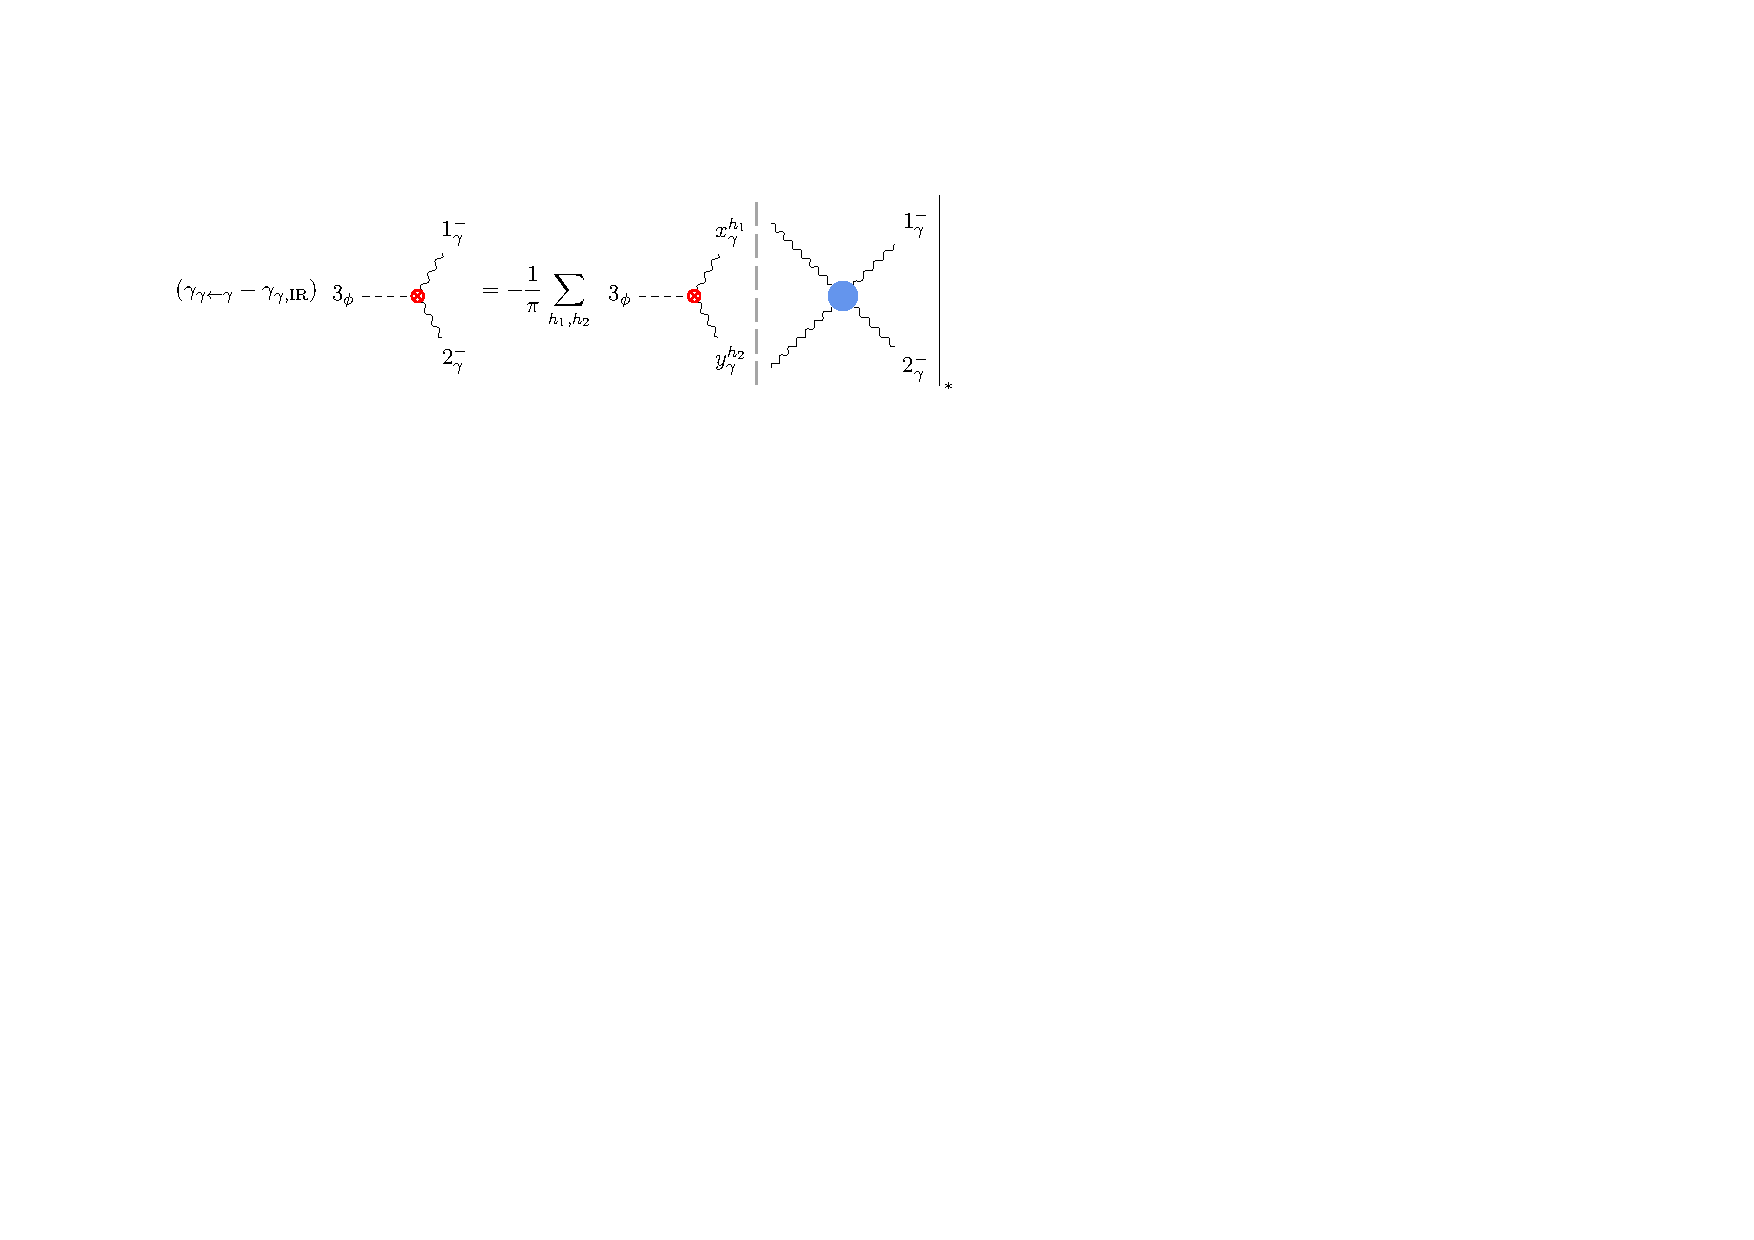
\includegraphics[page=1]{images/ALP_diagrams.pdf}
\caption[Diagrammatic formula for computing $\gamma_{\gamma \leftarrow \gamma}$]{Diagrammatic formula for computing $\gamma_{\gamma \leftarrow \gamma}$.}
\label{fig:ALPgamma_gammagamma}
\end{figure}

The form factor on the left reads
\begin{equation}
    F_\gamma|_*(1^-_\gamma,2^-_\gamma,3_\phi) = -2\frac{\agl{1}{2}^2}{\Lambda}\,,
\end{equation}
while the convolution on the right is expanded as
\begin{equation}
    (\mathcal M F_\gamma)|_*(1^-_\gamma,2^-_\gamma,3_\phi) = \sum_{h_1,h_2}\int \text{dLIPS}_2\, \mathcal M|_*(1^-_\gamma,2^-_\gamma;x_\gamma^{h_1},y^{h_2}_\gamma)F_\gamma|_*(x_\gamma^{h_1},y^{h_2}_\gamma,3_\phi)\,.
\end{equation}
Since the four-photon tree amplitude trivially vanishes for any choice of the helicities,
\begin{equation}
    \mathcal M|_*(1^-_\gamma,2^-_\gamma;x_\gamma^{h_1},y^{h_2}_\gamma) = 0\,,
\end{equation}
we obtain
\begin{equation}
    \gamma_{\gamma \leftarrow \gamma} = \gamma_{\gamma,\text{IR}} = \frac{e^2}{6\pi^2} \sum_f Q_f^2\,,
\end{equation}
where we exploited the expression for $\gamma_{\gamma,\text{IR}}$ derived in
Appendix~\ref{sec:ALPIRphigammagamma}, and $f$ runs over all the fermions of the theory.
We notice that we have successfully derived an expression that is equal to the anomalous
dimension of $e^2$, namely $(\mu/e^2)\, \text{d}e^2/\text{d}\mu$.

\paragraph{\texorpdfstring{$\gamma_{\gamma\leftarrow g}$}{gamma gamma from g}.}
The master formula associated with this matrix element reads
\begin{equation}
    \gamma_{\gamma\leftarrow g} F_\gamma|_*(1^-_\gamma,2^-_\gamma,3_\phi) = -\frac{1}{\pi}(\mathcal M F_g)|_*(1^-_\gamma,2^-_\gamma,3_\phi)
\end{equation}
and is represented in Figure~\ref{fig:ALPgamma_gammag}.

\begin{figure}[h!tb]
\centering
\includegraphics[page=2]{images/ALP_diagrams.pdf}
\caption[Diagrammatic formula for computing $\gamma_{\gamma\leftarrow g}$]{Diagrammatic formula for computing $\gamma_{\gamma\leftarrow g}$.}
\label{fig:ALPgamma_gammag}
\end{figure}

Also in this case the convolution on the right,
\begin{equation}
    (\mathcal M F_g)|_*(1^-_\gamma,2^-_\gamma,3_\phi) = \sum_{h_1,h_2}\int \text{dLIPS}_2\, \mathcal M|_*(1^-_\gamma,2^-_\gamma;x_{g^a}^{h_1},y^{h_2}_{g^b})F_g|_*(x_{g^a}^{h_1},y^{h_2}_{g^b},3_\phi)\,,
\end{equation}
vanishes since
\begin{equation}
    \mathcal M|_*(1^-_\gamma,2^-_\gamma;x_{g^a}^{h_1},y^{h_2}_{g^b}) = 0\,,
\end{equation}
and leads to
\begin{equation}
    \gamma_{\gamma\leftarrow g} = 0\,.
\end{equation}

\paragraph{\texorpdfstring{$\gamma_{\gamma\leftarrow S}$}{gamma gamma from S}.}
The equation linked to this matrix element is given by
\begin{equation}
    \gamma_{\gamma\leftarrow S_{ij}} F_\gamma|_*(1^-_\gamma,2^-_\gamma,3_\phi) = -\frac{1}{\pi}(\mathcal M F_{S_{ij}})|_*(1^-_\gamma,2^-_\gamma,3_\phi)
\end{equation}
and is represented as in Figure~\ref{fig:ALPgamma_gammaS}.

\begin{figure}[h!tb]
\centering
\includegraphics[page=3]{images/ALP_diagrams.pdf}
\caption[Diagrammatic formula for computing $\gamma_{\gamma\leftarrow S_{ij}}$]{Diagrammatic formula for computing $\gamma_{\gamma\leftarrow S_{ij}}$.}
\label{fig:ALPgamma_gammaS}
\end{figure}

From dimensional analysis, we expect
\begin{equation}
    \gamma_{\gamma\leftarrow S_{ij}}=0
\end{equation}
since $[\mathcal O_\gamma]-[\mathcal O_{S_{ij}}]=1$, which is in particular greater than $0$.
This is indeed consistent with the fact that the convolution
\begin{equation}
    (\mathcal M F_{S_{ij}})|_*(1^-_\gamma,2^-_\gamma,3_\phi) = \sum_{h_1,h_2}\int \text{dLIPS}_2\, \mathcal M|_*(1^-_\gamma,2^-_\gamma;x_{f_i}^{h_1},y^{h_2}_{\bar f_j})F_{S_{ij}}|_*(x_{f_i}^{h_1},y^{h_2}_{\bar f_j},3_\phi)
\end{equation}
vanishes due to
\begin{equation}
    \mathcal M|_*(1^-_\gamma,2^-_\gamma;x_{f_i}^{h_1},y^{h_2}_{\bar f_j})=0
\end{equation}
for any choice of $h_1$ and $h_2$.

\paragraph{\texorpdfstring{$\gamma_{\tilde\gamma \leftarrow \tilde\gamma}$, $\gamma_{\tilde\gamma \leftarrow \tilde g}$, and $\gamma_{\tilde\gamma \leftarrow P}$}{gamma gammatilde from gammatilde, gtilde, and P}.}
\label{par:ALPPhiFF}
The anomalous dimensions that contribute to the renormalization of $\phi F\widetilde F$ are
equal to those of $\phi FF$ up to signs that can be determined through the comments leading to
Eq.~\eqref{eq:ALPObs1}:
\begin{align}
    \gamma_{\tilde\gamma \leftarrow \tilde\gamma} &= \gamma_{\gamma \leftarrow \gamma} = \frac{e^2}{6\pi^2}\sum_f Q_f^2 \,,\\
    \gamma_{\tilde\gamma \leftarrow \tilde g} &= \gamma_{\gamma \leftarrow  g} = 0\,,\\
    \gamma_{\tilde\gamma \leftarrow P_{ij}} &= -\gamma_{\gamma \leftarrow S_{ij}} = 0\,.
\end{align}

An interesting feature of the on-shell, unitarity-based method we are employing is that it
makes some properties of the anomalous-dimension matrix manifest.
This is precisely the case for the operator $\phi FF$.
Based on pure symmetry arguments, indeed, one would expect this operator to renormalize like
the electromagnetic fine-structure constant at one-loop level.
The reason for this resides in the fact that the ALP is a pure SM gauge singlet, and hence
$\phi FF$ is expected to renormalize as $FF$.
In turn, as a consequence of Ward identities, this equals the renormalization of
$\alpha_{\text{em}}$.
Such a property is, however, not manifestly apparent at the level of Feynman diagrams.
On the other hand, it is immediately retrieved within the scope of the on-shell method.

\subsubsection{\texorpdfstring{$\phi GG$ and $\phi G\widetilde G$}{phi GG and phi G Gtilde}}
\label{sec:ALPphiGG}

\paragraph{\texorpdfstring{$\gamma_{g \leftarrow g}$}{gamma g from g}.}
The multiplicative renormalization effect of the ALP effective operator $\phi GG$ is encoded in
$\gamma_{g \leftarrow g}$, which can be derived from
\begin{equation}
     (\gamma_{g\leftarrow g}-\gamma_{g,\text{IR}}) F_g|_*(1^-_{g^a},2^-_{g^b},3_\phi) = -\frac{1}{\pi}(\mathcal M F_g)|_*(1^-_{g^a},2^-_{g^b},3_\phi)\,,
\end{equation}
schematized as in Figure~\ref{fig:ALPgamma_gg}.

\begin{figure}[h!tb]
\centering
\includegraphics[page=5]{images/ALP_diagrams.pdf}
\caption[Diagrammatic formula for computing $\gamma_{g\leftarrow g}$]{Diagrammatic formula for computing $\gamma_{g\leftarrow g}$.}
\label{fig:ALPgamma_gg}
\end{figure}

The convolution is now given by
\begin{equation}
    (\mathcal M F_g)|_*(1^-_{g^a},2^-_{g^b},3_\phi) = \sum_{h_1,h_2}\int \text{dLIPS}_2 \, \mathcal M|_*(1^-_{g^a},2^-_{g^b};x^{h_1}_{g^c},y^{h_2}_{g^d})F_g|_*(x^{h_1}_{g^c},y^{h_2}_{g^d},3_\phi)\,,
\end{equation}
where the only contributing amplitude
\begin{equation}
    \mathcal M|_*(1^-_{g^a},2^-_{g^b};x^{-}_{g^c},y^{-}_{g^d})\delta^{cd} = -2C_Ag_s^2 \delta^{ab}\frac{\agl{1}{2}^4}{\agl{1}{x}\agl{x}{2}\agl{2}{y}\agl{y}{1}}
\end{equation}
is multiplied by
\begin{equation}
    F_g|_*(x^{-}_{g^c},y^{-}_{g^d},3_\phi) = -2\delta^{cd}\frac{\agl{x}{y}^2}{\Lambda}\,.
\end{equation}

\subparagraph{Angular integration.}
The calculation of the phase-space integral with the angular parameterization is as follows.
The product reads
\begin{equation}
    \mathcal M|_*(1^-_{g^a},2^-_{g^b};x^{-}_{g^c},y^{-}_{g^d})F_g|_*(x^{-}_{g^c},y^{-}_{g^d},3_\phi) = -4C_Ag_s^2 \delta^{ab} \frac{\agl{1}{2}^2}{\Lambda} \frac{1}{\cos^2\theta \sin^2\theta}\,,
\end{equation}
yielding
\begin{equation}
    (\mathcal M F_g)|_*(1^-_{g^a},2^-_{g^b},3_\phi) = -4C_Ag_s^2 \delta^{ab} \frac{\agl{1}{2}^2}{\Lambda} \frac{1}{16\pi}\int_0^{\pi/2}2 \sin\theta\cos\theta\,\text{d}\theta\, \frac{1}{\cos^2\theta \sin^2\theta}\,.
\end{equation}
Therefore, by making use of the expression for $\gamma_{g,\text{IR}}$ derived in
Appendix~\ref{sec:ALPIRphigg} and reported in Eq.~\eqref{eq:ALPgammaIRgluon_angular}, we obtain
\begin{align}
    \gamma_{g\leftarrow g} &= \gamma_{g,\text{IR}} - C_A\frac{g_s^2}{8\pi^2}  \int_0^{\pi/2}2\sin\theta\cos\theta \, \text{d}\theta \, \frac{1}{\cos^2\theta\sin^2\theta}\nonumber \\
    &= T_F\frac{g_s^2}{6\pi^2}\sum_f c_f^2 - C_A\frac{g_s^2}{8\pi^2}  \int_0^{\pi/2}2\sin\theta\cos\theta \, \text{d}\theta \, \frac{1 -\cos^8\theta- \sin^8\theta}{\cos^2\theta\sin^2\theta}\nonumber \\
    &= -\frac{g_s^2}{8\pi^2}\bigg(\frac{11}{3}C_A -\frac{4}{3}T_F\sum_fc_f^2\bigg)\,,
\end{align}
which is equal to the anomalous dimension of $g_s^2$, namely
$(\mu/g_s^2)\,\text{d}g_s^2/\text{d}\mu$, since $\sum_f c_f^2$ denotes the number of quarks.

\subparagraph{Stokes integration.}
The calculation of the phase-space integral with the Stokes parameterization is as follows.
The product reads
\begin{equation}
    \mathcal M|_*(1^-_{g^a},2^-_{g^b};x^{-}_{g^c},y^{-}_{g^d})F_g|_*(x^{-}_{g^c},y^{-}_{g^d},3_\phi) = -4C_Ag_s^2 \delta^{ab} \frac{\agl{1}{2}^2}{\Lambda} \frac{(1+z\bar z)^2}{z\bar z }
\end{equation}
and vanishes after performing the Stokes integration.
Therefore, also in this case, the anomalous dimension is given by $\gamma_{g,\text{IR}}$,
derived in Appendix \ref{sec:ALPIRphigg} and reported in
Eq.\ \eqref{eq:ALPgammaIRgluon_stokes}:
\begin{equation}
    \gamma_{g\leftarrow g} = \gamma_{g,\text{IR}}
    = -\frac{g_s^2}{8\pi^2}\bigg(\frac{11}{3}C_A -\frac{4}{3}T_F\sum_fc_f^2\bigg)\,.
\end{equation}

\paragraph{\texorpdfstring{$\gamma_{g\leftarrow \gamma}$}{gamma g from gamma}.}
The master formula for computing $\gamma_{g\leftarrow \gamma}$ is
\begin{equation}
    \gamma_{g\leftarrow \gamma} F_g|_*(1^-_{g^a},2^-_{g^b},3_\phi) = -\frac{1}{\pi}(\mathcal M F_\gamma)|_*(1^-_{g^a},2^-_{g^b},3_\phi)\,,
\end{equation}
and its diagrammatic expression is reported in Figure~\ref{fig:ALPgamma_ggamma}.

\begin{figure}[h!tb]
\centering
\includegraphics[page=4]{images/ALP_diagrams.pdf}
\caption[Diagrammatic formula for computing $\gamma_{g\leftarrow \gamma}$]{Diagrammatic formula for computing $\gamma_{g\leftarrow \gamma}$.}
\label{fig:ALPgamma_ggamma}
\end{figure}

On the left, the form factor associated with $\phi GG$ reads
\begin{equation}
    F_g|_*(1^-_{g^a},2^-_{g^b},3_\phi) = -2\delta^{ab}\frac{\agl{1}{2}^2}{\Lambda}\,,
\end{equation}
and the convolution on the right is expanded as
\begin{equation}
    (\mathcal M F_\gamma)|_*(1^-_{g^a},2^-_{g^b},3_\phi) = \sum_{h_1,h_2}\int \text{dLIPS}_2 \, \mathcal M|_*(1^-_{g^a},2^-_{g^b};x^{h_1}_\gamma,y^{h_2}_\gamma)F_\gamma|_*(x^{h_1}_\gamma,y^{h_2}_\gamma,3_\phi)\,.
\end{equation}
Since the amplitudes trivially vanish,
\begin{equation}
    \mathcal M|_*(1^-_{g^a},2^-_{g^b};x^{h_1}_\gamma,y^{h_2}_\gamma) = 0\,,
\end{equation}
we obtain
\begin{equation}
    \gamma_{g\leftarrow \gamma} = 0\,.
\end{equation}

\paragraph{\texorpdfstring{$\gamma_{g\leftarrow S}$}{gamma g from S}.}
The formula corresponding to $\gamma_{g\leftarrow S_{ij}}$ is
\begin{equation}
    \gamma_{g\leftarrow S_{ij}} F_g|_*(1^-_{g^a},2^-_{g^b},3_\phi) = -\frac{1}{\pi}(\mathcal M F_{S_{ij}})|_*(1^-_{g^a},2^-_{g^b},3_\phi)
\end{equation}
and is reported diagrammatically in Figure~\ref{fig:ALPgamma_gS}.

\begin{figure}[h!tb]
\centering
\includegraphics[page=6]{images/ALP_diagrams.pdf}
\caption[Diagrammatic formula for computing $\gamma_{g\leftarrow S_{ij}}$]{Diagrammatic formula for computing $\gamma_{g\leftarrow S_{ij}}$.}
\label{fig:ALPgamma_gS}
\end{figure}

Also in this case, analogously to $\gamma_{\gamma\leftarrow S_{ij}}$, we expect
\begin{equation}
    \gamma_{g\leftarrow S_{ij}}=0
\end{equation}
because $[\mathcal O_g]-[\mathcal O_{S_{ij}}]=1>0$.
This is indeed consistent with the fact that the convolution
\begin{equation}
    (\mathcal M F_{S_{ij}})|_*(1^-_{g^a},2^-_{g^b},3_\phi) = \sum_{h_1,h_2}\int \text{dLIPS}_2\, \mathcal M|_*(1^-_{g^a},2^-_{g^b};x_{f_i^I}^{h_1},y^{h_2}_{\bar f_j^J})F_{S_{ij}}|_*(x_{f_i^I}^{h_1},y^{h_2}_{\bar f_j^J},3_\phi)
\end{equation}
vanishes due to
\begin{equation}
    \mathcal M|_*(1^-_{g^a},2^-_{g^b};x_{f_i^I}^{h_1},y^{h_2}_{\bar f_j^J})=0
\end{equation}
for any choice of $h_1$ and $h_2$.

\paragraph{\texorpdfstring{$\gamma_{\tilde g \leftarrow \tilde\gamma}$, $\gamma_{\tilde g \leftarrow \tilde g}$, and $\gamma_{\tilde g \leftarrow P}$}{gamma gtilde from gammatilde, gtilde, and P}.}
\label{par:ALPPhiGG}
Once again, the anomalous dimensions that contribute to the renormalization of
$\phi G\widetilde G$ are equal to those of $\phi GG$ up to signs that can be determined through
the comments leading to Eq.~\eqref{eq:ALPObs1}:
\begin{align}
    \gamma_{\tilde g \leftarrow \tilde \gamma } &= \gamma_{ g \leftarrow  \gamma } = 0\,,\\
    \gamma_{\tilde g \leftarrow \tilde g } &= \gamma_{ g \leftarrow  g } = -\frac{g_s^2}{8\pi^2}\bigg(\frac{11}{3}C_A -\frac{4}{3}T_F\sum_fc_f^2\bigg) \,,\\
    \gamma_{\tilde g \leftarrow P_{ij} } &= -\gamma_{ g \leftarrow  S_{ij} } = 0\,.
\end{align}

\subsubsection{Renormalization-Group Equations}
\label{sec:ALPRGEcouplings}

In this section, we have successfully reproduced some known results in the literature regarding
the renormalization of the CP-violating ALP
Lagrangian~\cite{Bauer:2021mvw,Chala:2020wvs,DasBakshi:2023lca}.
Here we report a summary of our results:
\begin{gather}
    \mu\dv[]{\mathcal C_\gamma}{\mu} = \frac{e^2}{6\pi^2}\mathcal C_\gamma \sum_f Q_f^2\,,
    \qquad
    \mu\dv[]{\widetilde{\mathcal C}_\gamma}{\mu} = \frac{e^2}{6\pi^2}\widetilde{\mathcal C}_\gamma \sum_f Q_f^2\,,
    \\
    \mu\dv[]{\mathcal C_g}{\mu} = -\frac{g_s^2}{8\pi^2} \bigg(\frac{11}{3} C_A - \frac{4}{3}T_F \sum_f c_f^2\bigg) \mathcal C_g\,,
    \qquad
    \mu\dv[]{\widetilde{\mathcal C}_g}{\mu} = -\frac{g_s^2}{8\pi^2} \bigg(\frac{11}{3} C_A - \frac{4}{3}T_F \sum_f c_f^2\bigg) \widetilde{\mathcal C}_g \,,
    \\
    \mu\dv[]{\mathcal Y_S^{ij}}{\mu} = -\frac{3}{8\pi^2}\left(e^2Q_f^2+C_Fg_s^2c_f^2 \right)\mathcal Y_S^{ij} + \frac{3}{2\pi^2}\frac{m_i}{\Lambda}\left(e^2Q_f^2 \mathcal C_\gamma + C_F g_s^2 c_f^2 \mathcal C_g\right)\delta^{ij}\,,\\
    \mu\dv[]{\mathcal Y_P^{ij}}{\mu} = -\frac{3}{8\pi^2}\left(e^2Q_f^2 +C_Fg_s^2c_f^2 \right)\mathcal Y_P^{ij} - \frac{3}{2\pi^2}\frac{m_i}{\Lambda}\left(e^2Q_f^2 \widetilde{\mathcal C}_\gamma + C_F g_s^2 c_f^2 \widetilde{\mathcal C}_g\right)\delta^{ij}\,.
\end{gather}

%%%%%%%%%%%%%%%%
\subsection{Renormalization of Standard Model Effective Operators Below the Electroweak Scale}
\label{sec:ALPLEFT}
%%%%%%%%%%%%%%%%

The phenomenological consequences of the ALP-SM interactions encoded in
Eq.~\eqref{eq:ALPLag} are rich and diverse.
Of particular interest among these are the indirect effects on precision observables that are
induced by the virtual exchange of an ALP.
Such precision observables entail not only CP-violating probes, such as the electric dipole
moment of particles, nucleons, nuclei, and molecules, but also CP-conserving ones, as for
instance the anomalous magnetic moment of leptons~\cite{Marciano:2016yhf,DiLuzio:2020oah}.
Since the impact on these physical observables is generated at the quantum level, a natural
expectation is that their size can be determined by the leading logarithms that emerge from the
solution of the RGEs.
This expectation is rooted in the large separation of scales between the energies at which
experiments are performed and those at which the effective Lagrangian is defined.

The resulting CP-even $SU(3)_c \times U(1)_{\text{em}}$ invariant Lagrangian,
$\mathcal{L}^{\text{even}}_{\text{CP}}$, that is generated by integrating out the ALP at
one-loop level reads
\begin{align}
\label{eq:ALPCPELag}
 \mathcal{L}^{\text{even}}_{\text{CP}} &=
\frac{c_{\rm M}^{ij}}{\Lambda} \, \bar{f}_i \sigma^{\mu\nu} f_j \, F_{\mu\nu} +  \frac{c_{\rm CM}^{ij}}{\Lambda} \, \bar{f}_i \sigma^{\mu\nu} T^a f_j \, G^a_{\mu\nu} + \frac{D_G}{3\Lambda^2} f^{abc} G_\mu^{a \nu} G_{\nu}^{b \rho} G_{\rho}^{c \mu} \nonumber \\
& \quad +
\frac{c_{LL1}^{ijkl}}{\Lambda^2}(\bar f_{Li} \gamma^\mu f_{Lj})(\bar f'_{Lk}\gamma_\mu f'_{Ll}) + \frac{c_{LL8}^{ijkl}}{\Lambda^2}(\bar f_{Li} \gamma^\mu T^a f_{Lj})(\bar f'_{Lk}\gamma_\mu T^a f'_{Ll})\nonumber \\
& \quad +
\frac{c_{RR1}^{ijkl}}{\Lambda^2}(\bar f_{Ri} \gamma^\mu f_{Rj})(\bar f'_{Rk}\gamma_\mu f'_{Rl}) +
\frac{c_{RR8}^{ijkl}}{\Lambda^2}(\bar f_{Ri} \gamma^\mu T^a f_{Rj})(\bar f'_{Rk}\gamma_\mu T^a f'_{Rl})\nonumber \\
& \quad +
\frac{c_{LR1}^{ijkl}}{\Lambda^2}(\bar f_{Li} \gamma^\mu f_{Lj})(\bar f'_{Rk}\gamma_\mu f'_{Rl}) +
\frac{c_{LR8}^{ijkl}}{\Lambda^2}(\bar f_{Li} \gamma^\mu T^a f_{Lj})(\bar f'_{Rk}\gamma_\mu T^a f'_{Rl})
\,.
\end{align}
The corresponding CP-odd Lagrangian, $\mathcal{L}^{\text{odd}}_{\text{CP}}$, is given by
\begin{align}
\label{eq:ALPCPOLag}
 \mathcal{L}^{\text{odd}}_{\text{CP}} =
 \frac{c_{\rm E}^{ij}}{\Lambda} \, \bar{f}_i \sigma^{\mu\nu} i\gamma_5 f_j \, F_{\mu\nu} +  \frac{c_{\rm CE}^{ij}}{\Lambda} \, \bar{f}_i \sigma^{\mu\nu} i\gamma_5 T^a f_j \, G^a_{\mu\nu} + \frac{d_G}{3\Lambda^2} f^{abc} G_\mu^{a \nu} G_{\nu}^{b \rho} \widetilde G_{\rho}^{c \mu}\,.
\end{align}
Here, $\sigma_{\mu\nu} = \frac{i}{2}[\gamma_\mu,\gamma_\nu]$.
Notice that in the above Lagrangians we have neglected operators which emerge by integrating
out the ALP at tree level, such as $(\bar{f} f)( \bar{f}' f')$, $GGGG$, and so on.
In fact, in this case, RGE effects are fully accounted for by evaluating the effective ALP
couplings of Eqs.~\eqref{eq:ALPLagA} and \eqref{eq:ALPLagB} at the ALP mass scale.

The objective of this section is to evaluate the Wilson coefficients of the above Lagrangians
that are generated by running effects from $\Lambda$ down to the ALP mass scale.

\subsubsection{\texorpdfstring{$GG\widetilde G$ and $GGG$}{GG Gtilde and GGG}}
\label{sec:ALPGGG}

\paragraph{\texorpdfstring{$\gamma_{\tilde G^3\leftarrow g,\tilde g}$}{gamma G3tilde from g, gtilde}.}
We define the Weinberg dimension-six operator as
\begin{equation}
    \mathcal O_{\tilde G^3} = \frac{1}{3}f^{abc}G_\mu^{a \nu} G_{\nu}^{b \rho} \widetilde G_{\rho}^{c \mu}\,.
\end{equation}
The renormalization of the corresponding Wilson coefficient induced by the operators $\phi GG$
and $\phi G\widetilde G$ at one-loop order can be evaluated from
\begin{equation}\label{eq:ALPmastertildeG3}
    \gamma_{\tilde G^3\leftarrow g,\tilde g}F_{\tilde G^3}|_*(1^-_{g^a},2^-_{g^b},3^-_{g^c})=-\frac{1}{\pi}\left. \frac{\partial}{\partial \mathcal C_g} \right|_{\mathcal C_g = 0} (\mathcal M F_{\tilde g})|_{*,\mathcal C_g \neq  0}(1^-_{g^a},2^-_{g^b},3^-_{g^c})\,,
\end{equation}
which diagrammatically reads as in Figure~\ref{fig:ALPgammatildeG3}.

\begin{figure}[h!tb]
\centering
\includegraphics[page=9]{images/ALP_diagrams.pdf}
\caption[Diagrammatic formula for computing $\gamma_{\tilde G^3\leftarrow g,\tilde g}$]{Diagrammatic formula for computing $\gamma_{\tilde G^3\leftarrow g,\tilde g}$.}
\label{fig:ALPgammatildeG3}
\end{figure}

The minimal form factor of $\mathcal O_{\tilde G^3}$ reads
\begin{equation}
    F_{\tilde G^3}|_*(1^-_{g^a},2^-_{g^b},3^-_{g^c})=\frac{\sqrt 2}{\Lambda^2}f^{abc}\agl{1}{2}\agl{2}{3}\agl{3}{1}\,,
\end{equation}
while the convolution can be written as
\begin{equation}
    (\mathcal M F_{\tilde g})|_{*,\mathcal C_g \neq  0}(1^-_{g^a},2^-_{g^b},3^-_{g^c}) = 3 \sum_{h}\int \text{dLIPS}_2\, \mathcal{M}|_{*,\mathcal C_g \neq  0}(1^-_{g^a},2^-_{g^b};x_\phi,y^h_{g^d})
    F_{\tilde g}|_*(x_\phi,y^h_{g^d},3^-_{g^c})\,,
\end{equation}
where the factor $3$ accounts for all the permutations of the external gluons.
The only helicity $h$ that gives a non-zero contribution is the negative one, since
$F_{\tilde g}|_*(x_\phi,y^+_{g^d},3^-_{g^c}) = 0$.
The amplitude with $\mathcal C_g\neq 0$ and all the other Wilson coefficients turned off, and
the minimal form factor of $\mathcal O_{\tilde g}$, are, respectively, given by
\begin{align}
    \mathcal{M}|_{*,\mathcal C_g \neq  0}(1^-_{g^a},2^-_{g^b};x_\phi,y^-_{g^d}) &= 2i\sqrt{2}g_s \frac{\mathcal C_g}{\Lambda}f^{abd}\frac{ \agl{1}{2}^3 }{ \agl{1}{y} \agl{2}{y}}\,,\\
    F_{\tilde g}|_*(x_\phi,y^-_{g^d},3^-_{g^c}) &= -\frac{2i}{\Lambda}\delta^{cd}\agl{3}{y}^2\,.
\end{align}

\subparagraph{Angular integration.}
Using the angular parameterization for the phase-space integral, the amplitude reads
\begin{equation}\label{eq:ALPamplitudeCg}
    \mathcal{M}|_{*,\mathcal C_g \neq  0}(1^-_{g^a},2^-_{g^b};x_\phi,y^-_{g^d}) = -2i\sqrt{2}g_s \frac{\mathcal C_g}{\Lambda}f^{abd}\agl{1}{2}\frac{1}{ \cos\theta\sin\theta}e^{i\varphi}\,.
\end{equation}
The integration in the azimuthal angle $\varphi$ only involves
\begin{align}
    \int_0^{2\pi}\frac{\text{d}\varphi}{2\pi}\,F_{\tilde g}|_*(x_\phi,y^-_{g^d},3^-_{g^c}) e^{i\varphi} &=
    -\frac{2i}{\Lambda}\delta^{cd}\int_0^{2\pi}\frac{\text{d}\varphi}{2\pi}\, (\agl{3}{1}e^{-i\varphi}\sin\theta + \agl{3}{2}\cos\theta)^2e^{i\varphi}
    \nonumber \\&=\frac{4i}{\Lambda}\delta^{cd}\agl{2}{3}\agl{3}{1}\cos\theta\sin\theta\,,\label{eq:ALPphiintegral}
\end{align}
where $\int_0^{2\pi} \text{d}\varphi\,e^{in\varphi}=2\pi\delta_{0n}$ has been used.
Therefore, the $\theta$ dependences of Eqs.~\eqref{eq:ALPamplitudeCg} and
\eqref{eq:ALPphiintegral} cancel each other, and we are left with a trivial integral in
$\theta$, which leads to
\begin{align}
    (\mathcal M F_{\tilde g})|_{*,\mathcal C_g \neq  0}(1^-_{g^a},2^-_{g^b},3^-_{g^c}) &= 3\times 8\sqrt 2 g_s \frac{\mathcal C_g}{\Lambda^2}f^{abc}\agl{1}{2}\agl{2}{3} \agl{3}{1} \frac{1}{8\pi}\int_0^{\pi/2}2\sin\theta\cos\theta\,\text{d}\theta \nonumber \\
    &= \frac{3\sqrt{2}}{\pi\Lambda^2} g_s\mathcal  C_gf^{abc} \agl{1}{2}\agl{2}{3} \agl{3}{1}\,.
\end{align}

\subparagraph{Stokes integration.}
Using the Stokes parameterization for the phase-space integral, the amplitude reads
\begin{equation}
    \mathcal{M}|_{*,\mathcal C_g \neq  0}(1^-_{g^a},2^-_{g^b};x_\phi,y^-_{g^d}) = 2i\sqrt{2}g_s \frac{\mathcal C_g}{\Lambda}f^{abd}\agl{1}{2}\frac{1+z\bar z}{ z}\,,
\end{equation}
which implies
\begin{equation}
    (\mathcal M F_{\tilde g})|_{*,\mathcal C_g \neq  0}(1^-_{g^a},2^-_{g^b},3^-_{g^c}) =  \frac{3\sqrt{2}}{\pi\Lambda^2} g_s\mathcal  C_gf^{abc} \agl{1}{2}\agl{2}{3} \agl{3}{1}\,.
\end{equation}
Finally, from the master formula of Eq.~\eqref{eq:ALPmastertildeG3}, we obtain
\begin{equation}
\label{eq:ALPgammatildeG3}
    \gamma_{\tilde G^3\leftarrow g,\tilde g} = -\frac{3g_s}{\pi^2}\,.
\end{equation}

\paragraph{\texorpdfstring{$\gamma_{G^3\leftarrow g, g}$ and $\gamma_{G^3\leftarrow \tilde g, \tilde g}$}{gamma G3 from gg and gtilde gtilde}.}
\label{par:ALPGGG}
The beta function associated with the Wilson coefficient of the CP-even operator
\begin{equation}
    \mathcal O_{G^3} = \frac{1}{3}f^{abc}G_\mu^{a \nu} G_{\nu}^{b \rho} G_{\rho}^{c \mu}
\end{equation}
receives contributions from double insertions of the operators $\phi GG$ and
$\phi G\widetilde G$.
The corresponding anomalous dimensions $\gamma_{ G^3\leftarrow g, g}$ and
$\gamma_{ G^3\leftarrow \tilde g,\tilde g}$ can be computed via
\begin{align}
    \gamma_{ G^3\leftarrow g, g}F_{ G^3}|_*(1^-_{g^a},2^-_{g^b},3^-_{g^c})&=-\frac{1}{\pi}\left. \frac{\partial}{\partial \mathcal C_g} \right|_{\mathcal C_g = 0} (\mathcal M F_{g})|_{*,\mathcal C_g \neq  0}(1^-_{g^a},2^-_{g^b},3^-_{g^c})\,, \\
    \gamma_{ G^3\leftarrow \tilde g,\tilde g}F_{ G^3}|_*(1^-_{g^a},2^-_{g^b},3^-_{g^c})&=-\frac{1}{\pi}\left. \frac{\partial}{\partial \widetilde{\mathcal{C}}_g} \right|_{\widetilde{\mathcal{C}}_g = 0} (\mathcal M F_{\tilde g})|_{*,\widetilde{\mathcal{C}}_g \neq  0}(1^-_{g^a},2^-_{g^b},3^-_{g^c})\,,
\end{align}
respectively, and both can be straightforwardly related to the anomalous dimension
$\gamma_{\tilde G^3\leftarrow g,\tilde g}$ in Eq.~\eqref{eq:ALPgammatildeG3}.
Indeed, by taking into account that
\begin{align}
    F_{ G^3}|_*(1^-_{g^a},2^-_{g^b},3^-_{g^c}) &= -i F_{\tilde G^3}|_*(1^-_{g^a},2^-_{g^b},3^-_{g^c})\,, \\
    F_{g}|_*(x_\phi,y^-_{g^d},3^-_{g^c}) &=-i F_{\tilde g}|_*(x_\phi,y^-_{g^d},3^-_{g^c})\,,\\
    \frac{\partial}{\partial \widetilde{\mathcal{C}}_g}\mathcal{M}|_{*,\widetilde{\mathcal{C}}_g \neq  0}(1^-_{g^a},2^-_{g^b};x_\phi,y^-_{g^d})&= i \frac{\partial}{\partial \mathcal{C}_g} \mathcal{M}|_{*,\mathcal C_g \neq  0}(1^-_{g^a},2^-_{g^b};x_\phi,y^-_{g^d})\,,
\end{align}
we obtain
\begin{equation}
\label{eq:ALPGGG_AD}
    \gamma_{ G^3\leftarrow g, g} =- \gamma_{ G^3\leftarrow \tilde g, \tilde g} = \gamma_{ \tilde G^3\leftarrow g, \tilde g} = -\frac{3g_s}{\pi^2}\,.
\end{equation}

\subsubsection{\texorpdfstring{$\bar f \sigma\!\cdot\! F i\gamma_5 f$ and $\bar f \sigma\!\cdot\! F f$}{fbar sigma F i gamma5 f and fbar sigma F f}}
\label{sec:ALPdipole}

\paragraph{\texorpdfstring{$\gamma_{\mathrm{E}\leftarrow S,\tilde\gamma}$}{gamma E from S, gammatilde}.}
The first anomalous dimension $\gamma_{\text{E}_{ij}\leftarrow S_{kl},\tilde\gamma}$ of the
electric dipole operator
\begin{equation}
    \mathcal O_{\text{E}_{ij}} =
    \bar f_i \sigma^{\mu\nu}i\gamma_5 f_j F_{\mu\nu}
\end{equation}
is induced by the ALP operators $\phi\, \bar f_k f_l$ and $\phi F\widetilde F$.
The corresponding master formula reads
\begin{equation}
    \gamma_{\text{E}_{ij}\leftarrow S_{kl},\tilde\gamma} F_{\text{E}_{ij}}|_*(1^-_{f_i},2^-_{\bar f_j},3^-_\gamma) = -\frac{1}{\pi}\left.\frac{\partial}{\partial \mathcal Y_S^{kl}}\right|_{\mathcal Y_S^{kl}=0}(\mathcal M F_{\tilde\gamma})|_{*,\mathcal Y_S^{kl}\neq 0}(1^-_{f_i},2^-_{\bar f_j},3^-_\gamma)\,,
\end{equation}
whose diagrammatic expression is provided in Figure~\ref{fig:ALPgammaEDM}.

\begin{figure}[h!tb]
\centering
\includegraphics[width=\linewidth,page=10]{images/ALP_diagrams.pdf}
\caption[Diagrammatic formula for computing $\gamma_{\text{E}_{ij}\leftarrow S_{kl},\tilde\gamma}$]{Diagrammatic formula for computing $\gamma_{\text{E}_{ij}\leftarrow S_{kl},\tilde\gamma}$.}
\label{fig:ALPgammaEDM}
\end{figure}

On the left-hand side we have the form factor of the electric dipole operator
\begin{equation}
    F_{\text{E}_{ij}}|_*(1^-_{f_i},2^-_{\bar f_j},3^-_\gamma) = -\frac{2i \sqrt{2}}{\Lambda} \agl{1}{3}\agl{2}{3}\,,
\end{equation}
while, on the right-hand side, the convolution reads
\begin{equation}
    (\mathcal M F_{\tilde\gamma})|_{*,\mathcal Y_S^{kl}\neq 0}(1^-_{f_i},2^-_{\bar f_j},3^-_\gamma) = \sum_{h} \int \text{dLIPS}_2 \, \mathcal M|_{*,\mathcal Y_S^{kl}\neq 0}(1^-_{f_i},2^-_{\bar f_j};x_\phi,y^h_\gamma) F_{\tilde\gamma}|_*(x_\phi,y^h_\gamma,3_\gamma^-)\,,
\end{equation}
where the only non-vanishing amplitude is
\begin{equation}
    \mathcal M|_{*,\mathcal Y_S^{kl}\neq 0}(1^-_{f_i},2^-_{\bar f_j};x_\phi,y^-_\gamma) =  -\sqrt 2 eQ_f \mathcal Y_S^{kl}\delta^{ik}\delta^{jl} \frac{\agl{1}{2}^2}{\agl{1}{y}\agl{y}{2}}
\end{equation}
and is multiplied by
\begin{equation}
    F_{\tilde\gamma}|_*(x_\phi,y^-_\gamma,3_\gamma^-) = -\frac{2i}{\Lambda}\agl{3}{y}^2\,.
\end{equation}

\subparagraph{Angular integration.}
The calculation of the phase-space integral with the angular parameterization is as follows.
The amplitude reads
\begin{equation}
    \mathcal M|_{*,\mathcal Y_S^{kl}\neq 0}(1^-_{f_i},2^-_{\bar f_j};x_\phi,y^-_\gamma) =  -\sqrt 2 eQ_f \mathcal Y_S^{kl}\delta^{ik}\delta^{jl} \frac{1}{\cos\theta \sin\theta}e^{i\varphi}\,,
\end{equation}
and thus the integration in the azimuthal angle $\varphi$ only involves
\begin{equation}
    \int_0^{2\pi}\frac{\text{d}\varphi}{2\pi}\,F_{\tilde\gamma}|_*(x_\phi,y^-_\gamma,3_\gamma^-)e^{i\varphi} = - \frac{4i}{\Lambda}\agl{2}{3}\agl{1}{3}\cos\theta\sin\theta\,.
\end{equation}
Then, the remaining integral is simply
\begin{align}
    (\mathcal M F_{\tilde\gamma})|_{*,\mathcal Y_S^{kl}\neq 0}(1^-_{f_i},2^-_{\bar f_j},3^-_\gamma) &=  \frac{4 i\sqrt 2}{\Lambda}  eQ_f \mathcal Y_S^{kl}\delta^{ik}\delta^{jl}  \agl{2}{3}\agl{1}{3} \frac{1}{8\pi}\int_0^{\pi/2}2\sin\theta\cos\theta\,\text{d}\theta \nonumber \\
    &=  \frac{ i\sqrt 2}{2\pi\Lambda}  eQ_f \mathcal Y_S^{kl}\delta^{ik}\delta^{jl}  \agl{2}{3}\agl{1}{3}\,,
\end{align}
which leads to
\begin{equation}\label{eq:ALPgammaEfromSgammatilde}
    \gamma_{\text{E}_{ij}\leftarrow S_{kl},\tilde\gamma} =  \frac{eQ_f }{4\pi^2}\delta^{ik}\delta^{jl}\,.
\end{equation}

\subparagraph{Stokes integration.}
Using the Stokes parameterization, the amplitude reads
\begin{equation}
    \mathcal M|_{*,\mathcal Y_S^{kl}\neq 0}(1^-_{f_i},2^-_{\bar f_j};x_\phi,y^-_\gamma) =  \sqrt 2 eQ_f \mathcal Y_S^{kl}\delta^{ik}\delta^{jl} \frac{1+z \bar z}{z} \, ,
\end{equation}
and combining it with the form factor we get
\begin{equation}
    (\mathcal M F_{\tilde\gamma})|_{*,\mathcal Y_S^{kl}\neq 0}(1^-_{f_i},2^-_{\bar f_j},3^-_\gamma)
    =  \frac{ i\sqrt 2}{2\pi\Lambda}  eQ_f \mathcal Y_S^{kl}\delta^{ik}\delta^{jl}  \agl{2}{3}\agl{1}{3}\,,
\end{equation}
which leads to Eq.~\eqref{eq:ALPgammaEfromSgammatilde}.

\paragraph{\texorpdfstring{$\gamma_{\mathrm{E}\leftarrow P,\gamma}$}{gamma E from P, gamma}.}
The second anomalous dimension $\gamma_{\text{E}_{ij}\leftarrow P_{kl},\gamma}$, corresponding
to the insertion of the ALP operators $\phi\, \bar f_k i\gamma_5 f_l$ and $\phi FF$, can be
obtained from the master formula
\begin{equation}
    \gamma_{\text{E}_{ij}\leftarrow P_{kl},\gamma} F_{\text{E}_{ij}}|_*(1^-_{f_i},2^-_{\bar f_j},3^-_\gamma) = -\frac{1}{\pi}\left.\frac{\partial}{\partial \mathcal Y_P^{kl}}\right|_{\mathcal Y_P^{kl}=0}(\mathcal M F_{\gamma})|_{*,\mathcal Y_P^{kl}\neq 0}(1^-_{f_i},2^-_{\bar f_j},3^-_\gamma)\,,
\end{equation}
and, since the identities
\begin{align}
    F_{\gamma}|_*(x_\phi,y^-_\gamma,3_\gamma^-) &= -i F_{\tilde\gamma}|_*(x_\phi,y^-_\gamma,3_\gamma^-) \,,
    \label{eq:ALPF_gamma_identity}\\
    \frac{\partial}{\partial \mathcal Y_P^{kl}}\mathcal M|_{*,\mathcal Y_P^{kl}\neq 0}(1^-_{f_i},2^-_{\bar f_j};x_\phi,y^-_\gamma)&=-i \frac{\partial}{\partial \mathcal Y_S^{kl}} \mathcal M|_{*,\mathcal Y_S^{kl}\neq 0}(1^-_{f_i},2^-_{\bar f_j};x_\phi,y^-_\gamma)\label{eq:ALPamplitudeyukawaidentity}
\end{align}
hold, we can relate it to $\gamma_{\text{E}_{ij}\leftarrow S_{kl},\tilde\gamma}$, concluding
that
\begin{equation}
    \gamma_{\text{E}_{ij}\leftarrow P_{kl},\gamma} = - \gamma_{\text{E}_{ij}\leftarrow S_{kl},\tilde\gamma}= -\frac{eQ_f }{4\pi^2}\delta^{ik}\delta^{jl}\,.
\end{equation}

\paragraph{\texorpdfstring{$\gamma_{\mathrm{M}\leftarrow P,\tilde \gamma}$ and $\gamma_{\mathrm{M}\leftarrow S,\gamma}$}{gamma M from P, gammatilde and S, gamma}.}
The magnetic dipole operator is defined as
\begin{equation}
    \mathcal O_{\text{M}_{ij}} = \bar f_i \sigma^{\mu\nu}f_j F_{\mu\nu}\,,
\end{equation}
and the corresponding anomalous dimensions $\gamma_{\text{M}_{ij}\leftarrow S_{kl},\gamma}$ and
$\gamma_{\text{M}_{ij}\leftarrow P_{kl},\tilde\gamma}$ can be obtained from the master
formulae
\begin{align}
    \gamma_{\text{M}_{ij}\leftarrow S_{kl},\gamma} F_{\text{M}_{ij}}|_*(1^-_{f_i},2^-_{\bar f_j},3^-_\gamma) &= -\frac{1}{\pi}\left.\frac{\partial}{\partial \mathcal Y_S^{kl}}\right|_{\mathcal Y_S^{kl}=0}(\mathcal M F_{\gamma})|_{*,\mathcal Y_S^{kl}\neq 0}(1^-_{f_i},2^-_{\bar f_j},3^-_\gamma)\,, \\
    \gamma_{\text{M}_{ij}\leftarrow P_{kl},\tilde\gamma} F_{\text{M}_{ij}}|_*(1^-_{f_i},2^-_{\bar f_j},3^-_\gamma) &= -\frac{1}{\pi}\left.\frac{\partial}{\partial \mathcal Y_P^{kl}}\right|_{\mathcal Y_P^{kl}=0}(\mathcal M F_{\tilde\gamma})|_{*,\mathcal Y_P^{kl}\neq 0}(1^-_{f_i},2^-_{\bar f_j},3^-_\gamma)\,.
\end{align}
If we exploit the identity
\begin{equation}
    F_{\text{M}_{ij}}|_*(1^-_{f_i},2^-_{\bar f_j},3^-_\gamma) =i F_{\text{E}_{ij}}|_*(1^-_{f_i},2^-_{\bar f_j},3^-_\gamma)\,,
\end{equation}
as well as those in Eqs.~\eqref{eq:ALPF_gamma_identity} and
\eqref{eq:ALPamplitudeyukawaidentity}, we can relate both of them to
$\gamma_{\text{E}_{ij}\leftarrow S_{kl},\tilde\gamma}$, concluding that
\begin{equation}
    \gamma_{\text{M}_{ij}\leftarrow P_{kl},\tilde\gamma}=
    \gamma_{\text{M}_{ij}\leftarrow S_{kl},\gamma} = -
    \gamma_{\text{E}_{ij}\leftarrow S_{kl},\tilde\gamma} = -\frac{eQ_f }{4\pi^2}\delta^{ik}\delta^{jl}\,.
\end{equation}

\subsubsection{\texorpdfstring{$\bar f \sigma\!\cdot\! G i\gamma_5 f$ and $\bar f \sigma\!\cdot\! G f$}{fbar sigma G i gamma5 f and fbar sigma G f}}
\label{sec:ALPchromoelectric_dipole_moment}

\paragraph{\texorpdfstring{$\gamma_{\mathrm{CE}\leftarrow S,\tilde g}$ and $\gamma_{\mathrm{CE}\leftarrow P, g}$}{gamma CE from S, gtilde and P, g}.}
The RGEs for the chromo-electric dipole operator
\begin{equation}
    \mathcal O_{\text{CE}_{ij}} = \bar f_i \sigma^{\mu\nu}i\gamma_5 T^a f_j G_{\mu\nu}^a
\end{equation}
are captured by the anomalous dimensions
$\gamma_{\text{CE}_{ij}\leftarrow S_{kl},\tilde g}$ and
$\gamma_{\text{CE}_{ij}\leftarrow P_{kl}, g}$.
The former corresponds to the insertion of the ALP operators $\phi\, \bar f_k f_l$ and
$\phi G\widetilde G$, while the latter is induced by
$\phi\, \bar f_k i \gamma_5 f_l$ and $\phi G G$.
They can be easily derived from $\gamma_{\text{E}_{ij}\leftarrow S_{kl},\tilde \gamma}$ and
$\gamma_{\text{E}_{ij}\leftarrow P_{kl}, \gamma}$, respectively, by replacing $eQ_f$ with
$g_s c_f$:
\begin{equation}
    \gamma_{\text{CE}_{ij}\leftarrow S_{kl},\tilde g} =- \gamma_{\text{CE}_{ij}\leftarrow P_{kl}, g}=  \frac{g_sc_f }{4\pi^2}\delta^{ik}\delta^{jl}\,.
\end{equation}

\paragraph{\texorpdfstring{$\gamma_{\mathrm{CM}\leftarrow S, g}$ and $\gamma_{\mathrm{CM}\leftarrow P,\tilde g}$}{gamma CM from S, g and P, gtilde}.}
Finally, concerning the chromomagnetic dipole operator
\begin{equation}
    \mathcal O_{\text{CM}_{ij}} = \bar f_i \sigma^{\mu\nu} T^a f_j G_{\mu\nu}^a\,,
\end{equation}
we can straightforwardly compute its anomalous dimensions from
$\gamma_{\text{M}_{ij}\leftarrow P_{kl},\tilde\gamma}$ and
$\gamma_{\text{M}_{ij}\leftarrow S_{kl},\gamma}$, by following the same prescription used for
the case of the chromoelectric dipole operator:
\begin{equation}
    \gamma_{\text{CM}_{ij}\leftarrow S_{kl}, g}=\gamma_{\text{CM}_{ij}\leftarrow P_{kl},\tilde g}= -\frac{g_sc_f }{4\pi^2}\delta^{ik}\delta^{jl}\,.
\end{equation}

\subsubsection{Four-Fermion Operators}
\label{sec:ALPLEFT4f}

\paragraph{\texorpdfstring{$\gamma_{LL1 \leftarrow \gamma, \gamma}$, $\gamma_{LL1 \leftarrow \tilde \gamma, \tilde \gamma}$, $\gamma_{RR1 \leftarrow \gamma, \gamma}$, and $\gamma_{RR1 \leftarrow \tilde \gamma, \tilde \gamma}$}{gamma LL1 and RR1 from two ALP-photon couplings}.}
Having defined the four-fermion operator
\begin{equation}
    \mathcal O_{LL1_{ijkl}} = (\bar f_{Li} \gamma^\mu f_{Lj})(\bar f'_{Lk}\gamma_\mu f'_{Ll})\,,
\end{equation}
whose minimal form factor is
\begin{equation}
    F_{LL1_{ijkl}}|_*(1^-_{f_i},2^+_{\bar f_j}, 3^-_{f'_k},4^+_{\bar f'_l}) = \frac{2}{\Lambda^2}\agl{1}{3}\sqr{4}{2}
\end{equation}
for $f\neq f'$, we first analyze its anomalous dimension as induced by two ALP-photon
couplings, i.e., $\gamma_{LL1_{ijkl} \leftarrow \gamma, \gamma}$ and
$\gamma_{LL1_{ijkl} \leftarrow \tilde \gamma, \tilde \gamma}$.
The master formula for the calculation of the former is
\begin{equation}
    \gamma_{LL1_{ijkl} \leftarrow \gamma, \gamma}  F_{LL1_{ijkl}}|_*(1^-_{f_i},2^+_{\bar f_j}, 3^-_{f'_k},4^+_{\bar f'_l}) = -\frac{1}{\pi}
    \left.\frac{\partial}{\partial \mathcal C_\gamma}\right|_{\mathcal C_\gamma = 0}
    (\mathcal M F_\gamma)|_{*,\mathcal C_\gamma \neq 0} (1^-_{f_i},2^+_{\bar f_j}, 3^-_{f'_k},4^+_{\bar f'_l})\,,
\end{equation}
whose diagram is shown in Figure~\ref{fig:ALP4fermion}.

\begin{figure}[h!tb]
\centering
\includegraphics[width=\linewidth,page=15]{images/ALP_diagrams.pdf}
\caption[Diagrammatic formula for computing $\gamma_{LL1_{ijkl} \leftarrow \gamma, \gamma}$]{Diagrammatic formula for computing $\gamma_{LL1_{ijkl} \leftarrow \gamma, \gamma}$.}
\label{fig:ALP4fermion}
\end{figure}

As for $\gamma_{LL1_{ijkl} \leftarrow \tilde\gamma, \tilde\gamma}$,
$\gamma_{RR1_{ijkl} \leftarrow \gamma, \gamma}$, and
$\gamma_{RR1_{ijkl} \leftarrow \tilde\gamma, \tilde\gamma}$, they are equal to
$\gamma_{LL1_{ijkl} \leftarrow \gamma, \gamma}$ --- including the sign --- given the
aforementioned considerations.

The convolution on the right can be expanded as
\begin{align}
    (\mathcal M F_\gamma)|_{*,\mathcal C_\gamma \neq 0} (1^-_{f_i},2^+_{\bar f_j}, 3^-_{f'_k},4^+_{\bar f'_l}) &= \sum_h \int \text{dLIPS}_2 \Big[ \mathcal M|_{*,\mathcal C_\gamma \neq 0}(3^-_{f'_k},4^+_{\bar f'_l}; x_{\gamma}^h , y_\phi) F_{\gamma}|_*(1^-_{f_i},2^+_{\bar f_j},x_{\gamma}^h , y_\phi) \nonumber \\
    &\quad +
    \mathcal M|_{*,\mathcal C_\gamma \neq 0}(1^-_{f_i},2^+_{\bar f_j}; x_{\gamma}^h , y_\phi) F_{\gamma}|_*(3^-_{f'_k},4^+_{\bar f'_l},x_{\gamma}^h , y_\phi)
    \Big]\,,
\end{align}
where, for the $h=-$ configuration, we have
\begin{align}
    \mathcal M|_{*,\mathcal C_\gamma \neq 0}(3^-_{f'_k},4^+_{\bar f'_l}; x_{\gamma}^- , y_\phi) &= \frac{2\sqrt{2}}{\Lambda}e Q_{f'}\mathcal C_\gamma\delta^{kl} \frac{\sqr{4}{x}^2}{\sqr{4}{3}}\,,\\
    F_{\gamma}|_*(1^-_{f_i},2^+_{\bar f_j},x_{\gamma}^- , y_\phi) &= \frac{2\sqrt{2}}{\Lambda}e Q_{f}\delta^{ij} \frac{\agl{1}{x}^2}{\agl{1}{2}}  \,.
\end{align}
Thus, the only integral to perform is
\begin{equation}
    \int \text{dLIPS}_2 \, \agl{1}{x}^2 \sqr{4}{x}^2 = \frac{1}{24\pi}\agl{1}{3}^2 \agl{4}{3}^2\,,
\end{equation}
which, after accounting for the $h=+$ configuration and permuting the fermions, leads to the
following expression for the convolution, valid for $f \neq f'$:
\begin{align}
    (\mathcal M F_\gamma)|_{*,\mathcal C_\gamma \neq 0} (1^-_{f_i},2^+_{\bar f_j}, 3^-_{f'_k},4^+_{\bar f'_l}) = - \frac{4e^2}{3\pi \Lambda^2}Q_f Q_{f'} \mathcal C_\gamma \delta^{ij} \delta^{kl} \agl{1}{3}\sqr{4}{2}\,.
\end{align}

Instead, for $f = f'$, the above expression holds if we substitute
$\delta^{ij} \delta^{kl} \to \delta^{ij} \delta^{kl} + \delta^{il} \delta^{kj}$, and, since the
form factor on the left of the master formula acquires an additional factor of $2$, the
anomalous-dimension elements can be compactly written as
\begin{align}
    \gamma_{LL1_{ijkl} \leftarrow \gamma,\gamma } &=
    \gamma_{LL1_{ijkl} \leftarrow \tilde\gamma, \tilde\gamma} =
    \gamma_{RR1_{ijkl} \leftarrow \gamma,\gamma } =
    \gamma_{RR1_{ijkl} \leftarrow \tilde\gamma, \tilde\gamma}\nonumber \\
    &= (1-\delta_{ff'})\frac{2e^2}{3\pi^2 } Q_f Q_{f'}  \delta^{ij} \delta^{kl} +   \delta_{ff'}\frac{e^2}{3\pi^2 } Q_f^2  \delta^{ij} \delta^{kl}\,.\label{eq:ALPLL1fromgammagamma}
\end{align}

\paragraph{\texorpdfstring{$\gamma_{LL1\leftarrow g,g}$, $\gamma_{LL1\leftarrow \tilde g, \tilde g}$, $\gamma_{RR1\leftarrow g,g}$, and $\gamma_{RR1\leftarrow \tilde g, \tilde g}$}{gamma LL1 and RR1 from two ALP-gluon couplings}.}
These anomalous dimensions are non-vanishing only if $f = f'$, given that in this case the
operator $(\bar f_{Li} \gamma^\mu T^a f_{Lj})(\bar f_{Lk} \gamma_\mu T^a f_{Ll})$ can
be written as a linear combination of $\mathcal O_{LL1}$ operators, i.e.,
\begin{equation}
    (\bar f_{Li} \gamma^\mu T^a f_{Lj})(\bar f_{Lk} \gamma_\mu T^a f_{Ll}) = \frac{1}{2}\!\left[(\bar f_{Lk} \gamma^\mu  f_{Lj})(\bar f_{Li} \gamma_\mu f_{Ll})-\frac{1}{N_c}
    (\bar f_{Li} \gamma^\mu  f_{Lj})(\bar f_{Lk} \gamma_\mu f_{Ll})
    \right]\!\,,
\end{equation}
as a consequence of the identity
$T^a_{IJ}T^a_{KL} = \frac{1}{2}(\delta_{KJ}\delta_{IL}-\frac{1}{N_c}\delta_{IJ}\delta_{KL})$.
This implies that
\begin{align}
    \gamma_{LL1_{ijkl} \leftarrow g,g } &=
    \gamma_{LL1_{ijkl} \leftarrow \tilde g, \tilde g} =
    \gamma_{RR1_{ijkl} \leftarrow g,g } =
    \gamma_{RR1_{ijkl} \leftarrow \tilde g, \tilde g}\nonumber \\
    &= \delta_{ff'}\frac{g_s^2}{6\pi^2}c_f^2 \bigg(
    \delta^{kj}\delta^{il}-\frac{1}{N_c}\delta^{ij}\delta^{kl}
    \bigg)\,.
\end{align}

\paragraph{\texorpdfstring{$\gamma_{LL8\leftarrow g,g}$, $\gamma_{LL8\leftarrow \tilde g, \tilde g}$, $\gamma_{RR8\leftarrow g,g}$, and $\gamma_{RR8\leftarrow \tilde g, \tilde g}$}{gamma LL8 and RR8 from two ALP-gluon couplings}.}
For these anomalous dimensions we can recycle the results already obtained.
Indeed, since we work with a basis where the operators
$(\bar f_{Li} \gamma^\mu T^a f_{Lj})(\bar f'_{Lk} \gamma_\mu T^a f'_{Ll})$ and
$(\bar f_{Ri} \gamma^\mu T^a f_{Rj})(\bar f'_{Rk} \gamma_\mu T^a f'_{Rl})$ are
considered only for $f\neq f'$, we can extract the term of
Eq.~\eqref{eq:ALPLL1fromgammagamma} proportional to $(1-\delta_{ff'})$ and apply the
substitution $e^2 Q_f Q_{f'} \to g_s^2 c_f c_{f'}$:
\begin{align}
    \gamma_{LL8_{ijkl} \leftarrow g,g } &=
    \gamma_{LL8_{ijkl} \leftarrow \tilde g, \tilde g} =
    \gamma_{RR8_{ijkl} \leftarrow g,g } =
    \gamma_{RR8_{ijkl} \leftarrow \tilde g, \tilde g}= \frac{2g_s^2}{3\pi^2 } c_f c_{f'}  \delta^{ij} \delta^{kl}\,.
\end{align}

\paragraph{\texorpdfstring{$\gamma_{LR1 \leftarrow \gamma,\gamma}$, $\gamma_{LR1 \leftarrow \tilde \gamma,\tilde \gamma}$, $\gamma_{LR8\leftarrow g,g}$, and $\gamma_{LR8\leftarrow \tilde g, \tilde g}$}{gamma LR1 and LR8}.}
As for the mixed-chirality four-fermion operators, the calculation of their anomalous
dimensions is completely analogous to that corresponding to the same-chirality four-fermion
operators.
Regarding $\gamma_{LR1_{ijkl} \leftarrow \gamma,\gamma}$ and
$\gamma_{LR1_{ijkl} \leftarrow \tilde \gamma,\tilde \gamma}$ we have
\begin{equation}
    \gamma_{LR1_{ijkl} \leftarrow \gamma,\gamma} = \gamma_{LR1_{ijkl} \leftarrow \tilde \gamma,\tilde \gamma} = \frac{2e^2}{3\pi^2}Q_f Q_{f'} \delta^{ij} \delta^{kl}\,,
\end{equation}
while for $\gamma_{LR8_{ijkl}\leftarrow g,g}$ and
$\gamma_{LR8_{ijkl} \leftarrow \tilde g, \tilde g}$
\begin{equation}
    \gamma_{LR8_{ijkl}\leftarrow g,g} = \gamma_{LR8_{ijkl} \leftarrow \tilde g, \tilde g} = \frac{2g_s^2}{3\pi^2}c_f c_{f'} \delta^{ij} \delta^{kl}\,.
\end{equation}

\subsubsection{Renormalization-Group Equations}
\label{sec:ALPRGELEFT}

In the following, we summarize our results for the RGEs of the
complete set of SM effective operators below the electroweak scale, as induced by the presence
of a CP-violating ALP:
\begin{gather}
    \mu \dv[]{d_G}{\mu} = - \frac{3g_s}{\pi^2}\mathcal{C}_g \widetilde{\mathcal{C}}_g\,,
    \qquad
    \mu \dv[]{D_G}{\mu} = -\frac{3g_s}{2\pi^2}\left(\mathcal{C}_g^2 - \widetilde{\mathcal{C}}_g^2\right)\,,
    \\
    \mu\dv[]{c_{\rm E}^{ij}}{\mu} =  \frac{e Q_f}{4 \pi^2} \left( \mathcal{Y}_S^{ij} \widetilde{\mathcal{C}}_\gamma-\mathcal{Y}_P^{ij} \mathcal{C}_\gamma  \right) \,,
    \qquad
    \mu\dv[]{c_{\rm M}^{ij}}{\mu} = - \frac{e Q_f}{4 \pi^2} \left(\mathcal{Y}_P^{ij} \widetilde{\mathcal{C}}_\gamma  + \mathcal{Y}_S^{ij} \mathcal{C}_\gamma\right) \,,
    \\
    \mu\dv[]{c_{\rm CE}^{ij}}{\mu} = \frac{g_s c_f}{4 \pi^2} \left( \mathcal{Y}_S^{ij} \widetilde{\mathcal{C}}_g-\mathcal{Y}_P^{ij} \mathcal{C}_g  \right) \,,
    \qquad
    \mu\dv[]{c_{\rm CM}^{ij}}{\mu} = -\frac{g_s c_f}{4 \pi^2} \left(\mathcal{Y}_P^{ij} \widetilde{\mathcal{C}}_g  + \mathcal{Y}_S^{ij} \mathcal{C}_g\right) \,,\\
    \begin{aligned}
    \mu\dv[]{c_{LL1}^{ijkl}}{\mu} &=  \delta_{ff'}\bigg[\frac{e^2Q_f^2}{6\pi^2}\left(\mathcal C_\gamma^2 + \widetilde{\mathcal C}_\gamma^2\right)\delta^{ij}\delta^{kl}+\frac{g_s^2c_f^2}{12\pi^2}\left(\mathcal C_g^2 + \widetilde{\mathcal C}_g^2\right)\bigg(\delta^{il}\delta^{kj}-\frac{1}{N_c}\delta^{ij}\delta^{kl}\bigg) \bigg] \\&\quad + (1-\delta_{ff'})\frac{e^2}{3\pi^2}Q_f Q_{f'}\left(\mathcal C_\gamma^2 + \widetilde{\mathcal C}_\gamma^2\right)\delta^{ij}\delta^{kl}\,,
    \end{aligned}\\
    \begin{aligned}
    \mu\dv[]{c_{RR1}^{ijkl}}{\mu} &= \delta_{ff'}\bigg[\frac{e^2Q_f^2}{6\pi^2}\left(\mathcal C_\gamma^2 + \widetilde{\mathcal C}_\gamma^2\right)\delta^{ij}\delta^{kl}+\frac{g_s^2c_f^2}{12\pi^2}\left(\mathcal C_g^2 + \widetilde{\mathcal C}_g^2\right)\bigg(\delta^{il}\delta^{kj}-\frac{1}{N_c}\delta^{ij}\delta^{kl}\bigg) \bigg] \\&\quad+ (1-\delta_{ff'})\frac{e^2}{3\pi^2}Q_f Q_{f'}\left(\mathcal C_\gamma^2 + \widetilde{\mathcal C}_\gamma^2\right)\delta^{ij}\delta^{kl}\,,
    \end{aligned}\\
    \mu\dv[]{c_{LL8}^{ijkl}}{\mu} = \frac{g_s^2}{3\pi^2}c_f c_{f'}\left(\mathcal C_g^2 + \widetilde{\mathcal C}_g^2\right)\delta^{ij}\delta^{kl}\,,
    \qquad
    \mu\dv[]{c_{RR8}^{ijkl}}{\mu} = \frac{g_s^2}{3\pi^2}c_f c_{f'}\left(\mathcal C_g^2 + \widetilde{\mathcal C}_g^2\right)\delta^{ij}\delta^{kl}\,,\\
    \mu\dv[]{c_{LR1}^{ijkl}}{\mu} = \frac{e^2}{3\pi^2}Q_f Q_{f'}\left(\mathcal C_\gamma^2 + \widetilde{\mathcal C}_\gamma^2\right)\delta^{ij}\delta^{kl}\,,
    \qquad
    \mu\dv[]{c_{LR8}^{ijkl}}{\mu} = \frac{g_s^2}{3\pi^2}c_f c_{f'}\left(\mathcal C_g^2 + \widetilde{\mathcal C}_g^2\right)\delta^{ij}\delta^{kl}\,.
\end{gather}

Our general findings improve and extend previous results in the
literature~\cite{Marciano:2016yhf,Galda:2023qjx,DiLuzio:2020oah}.
In particular, we reproduce the results of Ref.~\cite{Galda:2023qjx} in the limit of a CP-odd
ALP, where $\mathcal C_\gamma = \mathcal C_g = \mathcal Y_S^{ij} = 0$.
Moreover, we also agree with the results of Refs.~\cite{Marciano:2016yhf,DiLuzio:2020oah},
where only the running of $d_G$, $c_{\text{E}}^{ij}$, and $c_{\text{CE}}^{ij}$ was computed.

%%%%%%%%%%%%%%%%
\subsection{Renormalization of Standard Model Effective Operators Above the Electroweak Scale}
\label{sec:ALPSMEFT}
%%%%%%%%%%%%%%%%

In the previous sections, we focused on RGE effects below the electroweak scale, as they are
expected to be dominant in the low-energy phenomenology of CP-violating
ALPs~\cite{Marciano:2016yhf,DiLuzio:2020oah}.
Indeed, as long as these particles are considerably lighter than the electroweak scale, their
phenomenology is mainly driven by the operators in Eq.~\eqref{eq:ALPLag}, which are invariant
under the unbroken SM gauge group $SU(3)_c\times U(1)_\text{em}$.
The interactions of such particles with heavier states play a subdominant role on the
low-energy observables that constitute the main phenomenological probes of such a new-physics
candidate~\cite{DiLuzio:2020oah,DiLuzio:2023cuk}.
However, in view of embedding a CP-violating ALP in a UV-complete model, it is important to
keep track of its interactions with the SM fields in the unbroken phase.
These are encoded in the following Lagrangian:
\begin{align}
\mathcal{L}_\text{EFT} &= \widetilde{\mathcal{C}}_{G}\frac{\phi}{\Lambda} G_{\mu\nu}^a\widetilde{G}^{a\mu\nu} + \widetilde{\mathcal{C}}_{W}\frac{\phi}{\Lambda} W^I_{\mu\nu}\widetilde{W}^{I\mu\nu}+ \widetilde{\mathcal{C}}_{B}\frac{\phi}{\Lambda} B_{\mu\nu}\widetilde{B}^{\mu\nu}\nonumber \\
&\quad + \mathcal{C}_{G}\frac{\phi}{\Lambda} G_{\mu\nu}^aG^{a\mu\nu} + \mathcal{C}_{W}\frac{\phi}{\Lambda} W_{\mu\nu}^I W^{I\mu\nu}+ \mathcal{C}_{B}\frac{\phi}{\Lambda} B_{\mu\nu}B^{\mu\nu} \nonumber \\
&\quad + \frac{\phi}{\Lambda} \left(\overline{q}_p\widetilde{\mathcal{Y}}^{pr}_u\widetilde{H}u_r+ \overline{q}_p\widetilde{\mathcal{Y}}^{pr}_d H d_r+ \overline{\ell}_p\widetilde{\mathcal{Y}}^{pr}_e He_r + \text{H.c.}\right) + \mathcal{L}_{\text{SM}}\,,
\label{eq:ALPSMEFTLag}
\end{align}
where $\widetilde{\mathcal{Y}}_{f}$ with $f = u,d,e$ are generic $3 \times 3$ matrices, and
where
\begin{align}
\mathcal{L}_\text{SM} &= -\frac{1}{4}G_{\mu\nu}^aG^{a\mu\nu}-\frac{1}{4}W_{\mu\nu}^IW^{I\mu\nu}-\frac{1}{4}B_{\mu\nu}B^{\mu\nu}+(D_\mu H)^\dagger (D^\mu H)-\lambda \left(H^\dagger H-\frac{v^2}{2}\right)^2 \nonumber \\
&\quad + i \left(\overline \ell \gamma^\mu D_\mu \ell + \overline q \gamma^\mu D_\mu q + \overline e \gamma^\mu D_\mu e + \overline u \gamma^\mu D_\mu u + \overline d \gamma^\mu D_\mu d\right) \nonumber \\
&\quad - \left(Y_e^{pr} \overline \ell_p e_r H + Y_u^{pr} \overline q_p u_r \widetilde H + Y_d^{pr} \overline q_p d_r H + \text{H.c.}\right)\,,
\end{align}
with
$D_\mu = \partial_\mu - i g_1 y B_\mu - i g_2 \frac{\sigma^I}{2}W_\mu^I-i g_s T^a G^a_\mu$.
The hypercharge assignments are $y_\ell = -1/2$, $y_e = -1$, $y_q=1/6$, $y_u=2/3$,
$y_d = -1/3$, and $y_H = 1/2$.

The impact of the virtual exchange of a CP-violating ALP on the SMEFT operators, as induced by
the Lagrangian above, can be readily computed by making use of the on-shell method.
In this section we report our results, under the notation
\begin{equation}
\mathcal L_{\text{SMEFT}}^{(6)} = \frac{1}{\Lambda^2} \sum_i C_i \,Q_i \,,
\end{equation}
where the $C_i$ denote the Wilson coefficients of the SMEFT in the Warsaw
basis~\cite{Grzadkowski:2010es}.

Our results reproduce those of Ref.~\cite{Galda:2021hbr}, relative to a CP-odd ALP, and
generalize them to include interactions of a CP-even ALP.
In particular, as we will discuss systematically in the following, in our framework of a
CP-violating ALP we are forced to introduce and then renormalize dimension-six CP-odd
operators, which were not accounted for before.

\subsubsection{\texorpdfstring{Class $X^3$}{Class X3}}

Operators in this class include
\begin{align}
Q_G &= f^{abc} G_\mu^{a\nu}G_\nu^{b \rho}G_\rho^{c\mu}\,,  & Q_{\tildee{G}} &= f^{abc} \widetilde G_\mu^{a\nu}G_\nu^{b \rho}G_\rho^{c\mu}\,,  \\
Q_W &= \epsilon^{IJK} W_\mu^{I\nu}W_\nu^{J \rho}W_\rho^{K\mu}\,,  & Q_{\tildee{W}} &= \epsilon^{IJK} \widetilde{W}_\mu^{I\nu}W_\nu^{J \rho}W_\rho^{K\mu}\,.
\end{align}
The computation of the RGEs for this class of operators proceeds in complete analogy to the
renormalization of the same operators considered in Section~\ref{sec:ALPLEFT}.
We report here the results:
\begin{align}
\mu\dv[]{}{\mu}{C}_G &= \frac{g_s}{2\pi^2}   \left(\widetilde{\mathcal{C}}_{G}^2 - \mathcal{C}^2_{G} \right)\,, & \mu\dv[]{}{\mu}{C}_{\tildee{G}} &= -\frac{g_s}{\pi^2}  \,\widetilde{\mathcal{C}}_{G}\mathcal{C}_{G}\,,  \\
\mu\dv[]{}{\mu}{C}_W &=\frac{g_2}{2\pi^2}   \left(\widetilde{\mathcal{C}}_{W}^2 - \mathcal{C}^2_{W} \right)\,, & \mu\dv[]{}{\mu}{C}_{\tildee{W}} &= -\frac{g_2}{\pi^2} \, \widetilde{\mathcal{C}}_{W}\mathcal{C}_{W}  \,.
\end{align}

\subsubsection{\texorpdfstring{Class $X^2 H^2$}{Class X2H2}}

Operators in this class include
\begin{align}
Q_{HG} &= H^\dagger H \, G_{\mu\nu}^a G^{a\mu\nu}\,, & Q_{H\tildee{G}}&= H^\dagger H\,\widetilde{G}_{\mu\nu}^aG^{a\mu\nu}\,, \\
Q_{HW} &= H^\dagger H \, W_{\mu\nu}^I W^{I\mu\nu}\,, &Q_{H\tildee{W}}&= H^\dagger H\,\widetilde{W}_{\mu\nu}^I W^{I\mu\nu}\,,  \\
Q_{HB} &= H^\dagger H \, B_{\mu\nu}B^{\mu\nu}\,, &Q_{H\tildee{B}}&= H^\dagger H\,\widetilde{B}_{\mu\nu}B^{\mu\nu} \,,\\
Q_{HWB} &= H^\dagger \sigma^I H \, W_{\mu\nu}^I B^{\mu\nu}\,, & Q_{H\tildee W B}&= H^\dagger\sigma^I  H\,\widetilde{W}_{\mu\nu}^I B^{\mu\nu} \,.
\end{align}
The RGEs for the operators in this class can in principle receive contributions from all the
unitarity cuts in Figure~\ref{fig:ALPclassX2H2}.
However, it is easy to get convinced that only the leftmost unitarity cut can actually
contribute.
Indeed, in order to have a non-zero contribution to the operator $H^2 X^2$, the two external
gauge bosons must have the same helicity.
In addition to this, all the vector bosons involved in a dimension-five ALP-SM vertex must have
the same helicity as well.
As a consequence, the two virtual gauge bosons in the second and third diagrams must have the
same helicity.
While this is not a problem as far as the beyond-the-SM amplitude is concerned, it is
impossible to build a non-zero SM amplitude with two external Higgs fields and two gauge bosons
with the same helicities.
Hence, only the first diagram can possibly provide a non-null contribution to the
renormalization of the SMEFT operators in the class $X^2 H^2$. The results we find read
\begin{align}
\mu \dv[]{}{\mu} {C}_{HG} &= 0\,, & \mu \dv[]{}{\mu} {C}_{H\tildee{G}} &= 0\,,  \\
\mu \dv[]{}{\mu} {C}_{HW} &= -\frac{g_2^2}{8\pi^2}  \left(\widetilde{\mathcal{C}}_{W}^2 - \mathcal{C}^2_{W} \right)\,, & \mu \dv[]{}{\mu} {C}_{H\tildee{W}} &=  \frac{g_2^2}{4\pi^2}\,\mathcal{C}_{W} \widetilde{\mathcal{C}}_{W}\,,  \\
\mu \dv[]{}{\mu} {C}_{HB} &= -\frac{g_1^2}{8\pi^2}  \left(\widetilde{\mathcal{C}}_{B}^2 - \mathcal{C}^2_{B} \right)\,, & \mu \dv[]{}{\mu} {C}_{H\tildee{B}} &= \frac{g_1^2}{4\pi^2} \, \mathcal{C}_{B} \widetilde{\mathcal{C}}_{B}\,,    \\
\mu \dv[]{}{\mu} {C}_{HWB} &= -\frac{g_1 g_2}{4\pi^2}  \left(\widetilde{\mathcal{C}}_{W}\widetilde{\mathcal{C}}_{B} - \mathcal{C}_{W}\mathcal{C}_{B} \right)\,,
 &
 \mu \dv[]{}{\mu} {C}_{H\tildee{W}B} &= \frac{g_1 g_2}{4\pi^2}\left(\mathcal{C}_{W} \widetilde{\mathcal{C}}_{B}+ \mathcal{C}_{B} \widetilde{\mathcal{C}}_{W}\right)\,.
\end{align}

\begin{figure}[h!tb]
\centering
\begin{tikzpicture}
	\begin{feynman}[small]
		\node[red, dot](a);
		\vertex[right =  of a](b);
		\vertex[left =  of a](d);
		\vertex[below = 1.3 of a](f);
		\vertex[left = of f](g);
		\vertex[right = of f](h);
		\diagram*{
			(b) -- [scalar](a),
			(a) -- [photon](d),
			(f) -- [photon](a),
			(g) -- [charged scalar](f),
			(f) -- [charged scalar](h),
		};
	\end{feynman}
	\end{tikzpicture}
	\,
	\begin{tikzpicture}
	\draw[dashed,gray,very thick] (0.0, -0.7) -- (0.0, 0.7);
	\end{tikzpicture}
	\,
	\begin{tikzpicture}
	\begin{feynman}[small]
		\node[red, dot](a);
		\vertex[left = of a](b);
		\vertex[right = of a](d);
		\vertex[below = 1.3 of a](f);
		\vertex[left = of f](g);
		\vertex[right = of f](h);
		\diagram*{
			(b) -- [scalar](a),
			(a) -- [photon](d),
			(f) -- [photon](a),
			(g) -- [charged scalar](f),
			(f) -- [charged scalar](h),
		};
	\end{feynman} 
	\end{tikzpicture}
	\hfill 
	\begin{tikzpicture}
	\begin{feynman}[small]
		\vertex(a);
		\vertex[right =  of a](b);
		\vertex[left =  of a](d);
		\vertex[below = 1.3 of a](f);
		\vertex[left = of f](g);
		\vertex[right = of f](h);
		\diagram*{
			(b) -- [photon](a),
			(a) -- [charged scalar](d),
			(f) -- [charged scalar](a),
			(g) -- [charged scalar](f),
			(f) -- [photon](h),
		};
	\end{feynman}
	\end{tikzpicture}
	\,
	\begin{tikzpicture}
	\draw[dashed,gray,very thick] (0.0, -0.7) -- (0.0, 0.7);
	\end{tikzpicture}
	\,
	\begin{tikzpicture}
	\begin{feynman}[small]
		\node[red, dot](a);
		\vertex[left =  of a](b);
		\vertex[right = of a](d);
		\node[red, dot, below = 1.3 of a](f);
		\vertex[left = of f](g);
		\vertex[right = of f](h);
		\diagram*{
			(b) -- [photon](a),
			(a) -- [photon](d),
			(f) -- [scalar](a),
			(g) -- [photon](f),
			(f) -- [photon](h),
		};
	\end{feynman} 
	\end{tikzpicture}
    \hfill 
	\begin{tikzpicture}
	\begin{feynman}[small]
		\vertex(a);
		\vertex[above right =  of a](b);
		\vertex[ above left =  of a](d);
		\vertex[ below left = of a](g);
		\vertex[ below right = of a](h);
		\diagram*{
			(b) -- [photon](a),
			(a) -- [charged scalar](d),
			(g) -- [charged scalar](a),
			(a) -- [photon](h),
		};
	\end{feynman}
	\end{tikzpicture}
	\,
	\begin{tikzpicture}
	\draw[dashed,gray,very thick] (0.0, -0.7) -- (0.0, 0.7);
	\end{tikzpicture}
	\,
	\begin{tikzpicture}
	\begin{feynman}[small]
		\node[red, dot](a);
		\vertex[left =  of a](b);
		\vertex[right =  of a](d);
		\node[red, dot, below = 1.3  of a](f);
		\vertex[left = of f](g);
		\vertex[right = of f](h);
		\diagram*{
			(b) -- [photon](a),
			(a) -- [photon](d),
			(f) -- [scalar](a),
			(g) -- [photon](f),
			(f) -- [photon](h),
		};
	\end{feynman} 
	\end{tikzpicture}
\caption[Unitarity cuts for the renormalization of the class $X^2H^2$]{Unitarity cuts that contribute to the RGEs of the class $X^2H^2$. Dashed lines with an
arrow denote the hypercharge flow along a Higgs line, while dashed lines without arrows denote
an ALP. Only the first cut contributes to the RGE due to helicity arguments; see the main
text.}
\label{fig:ALPclassX2H2}
\end{figure}

\subsubsection{\texorpdfstring{Classes $H^6$ and $H^4D^2$}{Classes H6 and H4D2}}

The operators belonging to these classes are given by
\begin{align}
Q_H &= (H^\dagger H)^3\,, \\
Q_{H\Box} &= (H^\dagger H)\Box(H^\dagger H)\,, \\
Q_{HD} &= (H^\dagger D^\mu H)^*(H^\dagger D_\mu H)\,.
\end{align}
The relevant unitarity cuts for these classes of operators are reported in
Figure~\ref{fig:ALPclassH6}, and the corresponding RGEs read
\begin{align}
\mu \dv[]{}{\mu} {C}_{H} &= \frac{\lambda  g_2^2}{3\pi^2}  \left(\mathcal{C}_{W}^2+ \widetilde{\mathcal{C}}_{W}^2 \right)\,,  \\
\mu \dv[]{}{\mu} {C}_{H\Box} &= \frac{g_1^2}{24\pi^2}   \left(\mathcal{C}_{B}^2+ \widetilde{\mathcal{C}}_{B}^2\right)+ \frac{g_2^2}{8\pi^2}  \left(\mathcal{C}_{W}^2+ \widetilde{\mathcal{C}}_{W}^2\right)\,, \\
\mu \dv[]{}{\mu} {C}_{HD} &= \frac{g_1^2}{6\pi^2}   \left (\mathcal{C}_{B}^2+ \widetilde{\mathcal{C}}_{B}^2 \right)\,.
\end{align}

\begin{figure}[h!tb]
\centering
\begin{tikzpicture}
	\begin{feynman}[small]
		\vertex(a);
		\vertex[above left = of a](b);
		\vertex[below left = of a](c);
		\node[red, dot, right = of a ](d);
		\vertex[above right = of d](e);
		\vertex[below right = of d](f);
		\diagram*{
			(a) -- [charged scalar](b),
			(c) -- [charged scalar](a),
			(a) -- [photon](d),
			(d) -- [scalar](e),
			(d) -- [photon](f),
		};
	\end{feynman}
	\end{tikzpicture}
	\,
	\begin{tikzpicture}
	\draw[dashed,gray,very thick] (0.0, -0.7) -- (0.0, 0.7);
	\end{tikzpicture}
	\,
	\begin{tikzpicture}
	\begin{feynman}[small]
		\node[red, dot](a);
		\vertex[above left = of a](b);
		\vertex[below left = of a](c);
		\vertex[right = of a ](d);
		\vertex[above right = of d](e);
		\vertex[below right = of d](f);
		\diagram*{
			(a) -- [scalar](b),
			(c) -- [photon](a),
			(a) -- [photon](d),
			(d) -- [charged scalar](e),
			(f) -- [charged scalar](d),
		};
	\end{feynman} 
	\end{tikzpicture}
    \qquad \qquad \qquad 
    \begin{tikzpicture}
	\begin{feynman}[small]
		\vertex(a);
		\vertex[above left = of a](b);
		\vertex[below left = of a](c);
        \vertex[above left = 0.5 of a](a1);
        \vertex[below left = 0.5 of a1](a2);
        \vertex[ above right = 0.5 of a1](a3);
		\node[red, dot, right = of a ](d);
		\vertex[above right = of d](e);
		\vertex[below right = of d](f);
		\diagram*{
			(a) -- [charged scalar](a1),
            (a1) -- [charged scalar](b),
			(c) -- [charged scalar](a),
			(a) -- [photon](d),
			(d) -- [scalar](e),
			(d) -- [photon](f),
            (a1) -- [charged scalar](a2),
            (a3) -- [charged scalar](a1),
		};
	\end{feynman}
	\end{tikzpicture}
	\,
	\begin{tikzpicture}
	\draw[dashed,gray,very thick] (0.0, -0.7) -- (0.0, 0.7);
	\end{tikzpicture}
	\,
	\begin{tikzpicture}
	\begin{feynman}[small]
		\node[red, dot](a);
		\vertex[above left= of a](b);
		\vertex[below left= of a](c);
		\vertex[right = of a ](d);
		\vertex[above right = of d](e);
		\vertex[below right = of d](f);
		\diagram*{
			(a) -- [scalar](b),
			(c) -- [photon](a),
			(a) -- [photon](d),
			(d) -- [charged scalar](e),
			(f) -- [charged scalar](d),
		};
	\end{feynman} 
	\end{tikzpicture}
\caption[Unitarity cuts for the renormalization of the classes $H^6$ and $H^4D^2$]{Unitarity cuts that contribute to the RGEs of the classes $H^6$ and $H^4 D^2$. Dashed
lines with an arrow denote the hypercharge flow along a Higgs line, while dashed lines without
arrows denote an ALP.}
\label{fig:ALPclassH6}
\end{figure}

\subsubsection{\texorpdfstring{Class $\psi^2 H X$}{Class psi2 H X}}

In this class one finds the following dipole operators, accompanied by their Hermitian
conjugates:
\begin{align}
Q_{uB}^{pr} &= (\overline{q}_p\sigma^{\mu\nu} u_r)\,\widetilde H\,B_{\mu\nu}\,,  &Q_{uW}^{pr} &= (\overline{q}_p\sigma^{\mu\nu} \sigma^I u_r)\,\widetilde H\,W^I_{\mu\nu}\,, \\
 Q_{dB}^{pr} &= (\overline{q}_p\sigma^{\mu\nu} d_r)\,H\,B_{\mu\nu}\,,  & Q_{dW}^{pr} &= (\overline{q}_p\sigma^{\mu\nu} \sigma^I d_r)\,H\,W^I_{\mu\nu} \,,  \\
Q_{eB}^{pr} &= (\overline{\ell}_p\sigma^{\mu\nu} e_r)\,H\,B_{\mu\nu}\,, &Q_{eW}^{pr} &= (\overline{\ell}_p\sigma^{\mu\nu} \sigma^I e_r)\,H\,W^I_{\mu\nu}\,, \\
Q_{uG}^{pr} &= (\overline{q}_p\sigma^{\mu\nu} T^a u_r)\,\widetilde H\,G^a_{\mu\nu}\,, & Q_{dG}^{pr} &= (\overline{q}_p\sigma^{\mu\nu} T^a d_r)\,H\,G^a_{\mu\nu}\,.
\end{align}
The computations for this class of RGEs proceed in complete analogy to the case of dipole
operators in Section~\ref{sec:ALPLEFT}, and we report here the results:
\begin{align}
    \mu \dv[]{}{\mu}  C_{uB}^{pr} &=\frac{5 g_1}{48\pi^2}  \widetilde{\mathcal{Y}}_u^{pr} ({\mathcal{C}}_{B} + i  \widetilde{\mathcal{C}}_{B})\,,
    &
    \mu \dv[]{}{\mu}  C_{uW}^{pr} &=\frac{g_2}{16\pi^2}
 \widetilde{\mathcal{Y}}_u^{pr} ({\mathcal{C}}_{W} + i  \widetilde{\mathcal{C}}_{W})\,,  \\
 \mu \dv[]{}{\mu}  C_{dB}^{pr} &= -\frac{g_1}{48\pi^2}  \widetilde{\mathcal{Y}}_d^{pr} ({\mathcal{C}}_{B} + i  \widetilde{\mathcal{C}}_{B})\,,
    &
    \mu \dv[]{}{\mu}  C_{dW}^{pr} &= \frac{g_2}{16\pi^2}
 \widetilde{\mathcal{Y}}_d^{pr} ({\mathcal{C}}_{W} + i  \widetilde{\mathcal{C}}_{W})\,,  \\
 \mu \dv[]{}{\mu}  C_{eB}^{pr} &= -\frac{3g_1}{16\pi^2}  \widetilde{\mathcal{Y}}_e^{pr} ({\mathcal{C}}_{B} + i  \widetilde{\mathcal{C}}_{B})\,,
    &
    \mu \dv[]{}{\mu}  C_{eW}^{pr} &= \frac{g_2}{16\pi^2}
 \widetilde{\mathcal{Y}}_e^{pr} ({\mathcal{C}}_{W} + i  \widetilde{\mathcal{C}}_{W})\,,  \\
 \mu \dv[]{}{\mu}  C_{uG}^{pr} &= \frac{g_s }{4\pi^2}
 \widetilde{\mathcal{Y}}_u^{pr} ({\mathcal{C}}_{G} +i  \widetilde{\mathcal{C}}_{G})\,, &
 \mu \dv[]{}{\mu}  C_{dG}^{pr} &= \frac{g_s}{4\pi^2}
 \widetilde{\mathcal{Y}}_d^{pr} ({\mathcal{C}}_{G} +i  \widetilde{\mathcal{C}}_{G})\,.
\end{align}

\subsubsection{\texorpdfstring{Class $\psi^2 H^2 D$}{Class psi2 H2 D}}

In this class we find the following set of operators:
\begin{align}
Q_{H\ell}^{(1)pr} &= (H^\dagger i \overset{\leftrightarrow}{D}_\mu H)(\overline{\ell}_p \gamma^\mu \ell_r)\,,  &Q_{H \ell}^{(3)pr} &= (H^\dagger i \overset{\leftrightarrow}{D}{}^I_\mu H)(\overline{\ell}_p \sigma^I \gamma^\mu \ell_r) \,, \\
Q_{Hq}^{(1)pr} &= (H^\dagger i \overset{\leftrightarrow}{D}_\mu H)(\overline{q}_p \gamma^\mu q_r)\,,  &Q_{Hq}^{(3)pr} &= (H^\dagger i \overset{\leftrightarrow}{D}{}^I_\mu H)(\overline{q}_p \sigma^I \gamma^\mu q_r)\,, \\
Q_{He}^{pr} &= (H^\dagger i \overset{\leftrightarrow}{D}_\mu H)(\overline{e}_p \gamma^\mu e_r)\,,  &Q_{Hu}^{pr} &= (H^\dagger i \overset{\leftrightarrow}{D}_\mu H)(\overline{u}_p  \gamma^\mu u_r)\,, \\
Q_{Hd}^{pr} &= (H^\dagger i \overset{\leftrightarrow}{D}_\mu H)(\overline{d}_p \gamma^\mu d_r)\,,  &Q_{Hud}^{pr} &= i(\widetilde{H}^\dagger D_\mu H)(\overline{u}_p  \gamma^\mu d_r) \,.
\end{align}
The unitarity cuts relevant to the computation of the RGEs for this class of operators are
reported in Figure~\ref{fig:ALPclassespsi2}, and the corresponding RGEs read
\begin{align}
\mu \dv[]{}{\mu} {C}_{H\ell}^{(1)pr} &=\frac{1}{16\pi^2}\left[ \frac{1}{4}(\widetilde{\mathcal{Y}}_e\widetilde{\mathcal{Y}}_e^\dagger)^{pr} - \frac{4}{3} \,g_1^2 \,(\widetilde{\mathcal{C}}_{B}^2+ \mathcal{C}_{B}^2)\delta^{pr}\right] \,,  \\
\mu \dv[]{}{\mu} {C}_{H\ell}^{(3)pr} &=\frac{1}{16\pi^2}\left[ \frac{1}{4}(\widetilde{\mathcal{Y}}_e\widetilde{\mathcal{Y}}_e^\dagger)^{pr} + \frac{4}{3}\, g_2^2\,(\widetilde{\mathcal{C}}_{W}^2+ \mathcal{C}_{W}^2)\delta^{pr}\right] \,,  \\
\mu \dv[]{}{\mu} {C}_{He}^{pr} &=\frac{1}{16\pi^2}\left[ -\frac{1}{2}(\widetilde{\mathcal{Y}}_e^\dagger \widetilde{\mathcal{Y}}_e)^{pr} - \frac{8}{3} \,g_1^2 \,(\widetilde{\mathcal{C}}_{B}^2+ \mathcal{C}_{B}^2)\delta^{pr}\right] \,,  \\
\mu \dv[]{}{\mu} {C}_{Hq}^{(1)pr} &=\frac{1}{16\pi^2}\left[ \frac{1}{4}(\widetilde{\mathcal{Y}}_d\widetilde{\mathcal{Y}}_d^\dagger-\widetilde{\mathcal{Y}}_u\widetilde{\mathcal{Y}}_u^\dagger)^{pr} + \frac{4}{9} \,g_1^2 \,(\widetilde{\mathcal{C}}_{B}^2+ \mathcal{C}_{B}^2) \delta^{pr}\right] \,, \\
\mu \dv[]{}{\mu} {C}_{Hq}^{(3)pr} &=\frac{1}{16\pi^2}\left[ \frac{1}{4}(\widetilde{\mathcal{Y}}_d\widetilde{\mathcal{Y}}_d^\dagger+\widetilde{\mathcal{Y}}_u\widetilde{\mathcal{Y}}_u^\dagger)^{pr} + \frac{4}{3}\, g_2^2\,(\widetilde{\mathcal{C}}_{W}^2+ \mathcal{C}_{W}^2) \delta^{pr}\right] \,,  \\
\mu \dv[]{}{\mu} {C}_{Hd}^{pr} &=\frac{1}{16\pi^2}\left[ -\frac{1}{2}(\widetilde{\mathcal{Y}}_d^\dagger \widetilde{\mathcal{Y}}_d)^{pr} - \frac{8}{9} \,g_1^2 \,(\widetilde{\mathcal{C}}_{B}^2+ \mathcal{C}_{B}^2)\delta^{pr}\right] \,,  \\
\mu \dv[]{}{\mu} {C}_{Hu}^{pr} &=\frac{1}{16\pi^2}\left[ \frac{1}{2}(\widetilde{\mathcal{Y}}_u^\dagger \widetilde{\mathcal{Y}}_u)^{pr} + \frac{16}{9} \,g_1^2 \,(\widetilde{\mathcal{C}}_{B}^2+ \mathcal{C}_{B}^2)\delta^{pr}\right] \,,  \\
\mu \dv[]{}{\mu} {C}_{Hud}^{pr} &= -\frac{1}{16\pi^2}(\widetilde{\mathcal{Y}}_u^\dagger \widetilde{\mathcal{Y}}_d)^{pr}\,.
\end{align}

\begin{figure}[h!tb]
\centering
\begin{tikzpicture}
	\begin{feynman}[small]
		\node[red, dot](a);
		\vertex[above left = of a](b);
		\vertex[below left = of a](c);
		\vertex[below right = of a](e);
		\vertex[above right = of a](f);
		\diagram*{
			(b) -- [charged scalar](a),
			(c) -- [fermion](a),
			(a) -- [fermion](e),
			(a) -- [scalar](f),
		};
	\end{feynman}
	\end{tikzpicture}
	\,
	\begin{tikzpicture}
	\draw[dashed,gray,very thick] (0.0, -0.7) -- (0.0, 0.7);
	\end{tikzpicture}
	\,
	\begin{tikzpicture}
	\begin{feynman}[small]
		\node[red, dot](a);
		\vertex[left =  of a](b);
		\vertex[right =  of a](d);
		\vertex[below = 1.3 of a](f);
		\vertex[left = of f](g);
		\vertex[right = of f](h);
		\diagram*{
			(b) -- [scalar](a),
			(a) -- [photon](d),
			(f) -- [photon](a),
			(g) -- [fermion](f),
			(f) -- [fermion](h),
		};
	\end{feynman} 
	\end{tikzpicture}
        \hfill
    \begin{tikzpicture}
    	\begin{feynman}[small]
		\node[red, dot](a);
		\vertex[above left = of a](b);
		\vertex[below left = of a](c);
		\vertex[above right = of a](e);
		\vertex[below right = of a](f);
		\diagram*{
			(b) -- [charged scalar](a),
			(c) -- [fermion](a),
			(a) -- [fermion](e),
			(a) -- [scalar](f),
		};
	\end{feynman}
	\end{tikzpicture}
	\,
	\begin{tikzpicture}
	\draw[dashed,gray,very thick] (0.0, -0.7) -- (0.0, 0.7);
	\end{tikzpicture}
	\,
	\begin{tikzpicture}
	\begin{feynman}[small]
		\node[red, dot](a);
		\vertex[above left = of a](b);
		\vertex[below left = of a](c);
		\vertex[above right = of a](e);
		\vertex[below right = of a](f);
		\diagram*{
			(b) -- [fermion](a),
			(a) -- [scalar](c),
			(a) -- [charged scalar](e),
			(a) -- [fermion](f),
		};
	\end{feynman} 
	\end{tikzpicture}
    \hfill
    \begin{tikzpicture}
	\begin{feynman}[small]
		\vertex(a);
		\vertex[above left = of a](b);
		\vertex[below left = of a](c);
		\node[red, dot, right = of a ](d);
		\vertex[above right = of d](e);
		\vertex[below right = of d](f);
		\diagram*{
			(a) -- [fermion](b),
			(c) -- [fermion](a),
			(a) -- [photon](d),
			(d) -- [scalar](e),
			(d) -- [photon](f),
		};
	\end{feynman}
	\end{tikzpicture}
	\,
	\begin{tikzpicture}
	\draw[dashed,gray,very thick] (0.0, -0.7) -- (0.0, 0.7);
	\end{tikzpicture}
	\,
	\begin{tikzpicture}
	\begin{feynman}[small]
		\node[red, dot](a);
		\vertex[above left = of a](b);
		\vertex[below left = of a](c);
		\vertex[right = of a ](d);
		\vertex[above right = of d](e);
		\vertex[below right = of d](f);
		\diagram*{
			(a) -- [scalar](b),
			(c) -- [photon](a),
			(a) -- [photon](d),
			(d) -- [charged scalar](e),
			(f) -- [charged scalar](d),
		};
	\end{feynman} 
	\end{tikzpicture}
\caption[Unitarity cuts for the renormalization of the classes $\psi^2XH$ and $\psi^2H^2D$]{Unitarity cuts that contribute to the RGEs of the classes $\psi^2 XH$ and
$\psi^2 H^2 D$. Dashed lines with an arrow denote the hypercharge flow along a Higgs line,
while dashed lines without arrows denote an ALP.}
\label{fig:ALPclassespsi2}
\end{figure}

\subsubsection{\texorpdfstring{Class $\psi^2 H^3$}{Class psi2 H3}}

The three operators in this class read
\begin{align}
Q_{eH}^{pr} = (H^\dagger H)(\overline{\ell}_p e_r H)\,, \qquad Q_{uH}^{pr} = (H^\dagger H)(\overline{q}_p u_r \widetilde{H})\,, \qquad
Q_{dH}^{pr} = (H^\dagger H)(\overline{q}_p d_r H)\,.
\end{align}
The unitarity cuts relevant to the computation of the RGEs for such a class of operators are
depicted in Figure~\ref{fig:ALPclasspsi2H3}, and the associated RGEs read
\begin{equation}
 \mu \dv[]{}{\mu} {{C}}_{fH}^{pr} =-\frac{1}{16\pi^2}\left[ 2  ( \widetilde{\mathcal{Y}}_f {Y}_f^\dagger \widetilde{\mathcal{Y}}_f)^{pr} + \frac{1}{2} (\widetilde{\mathcal{Y}}_f \widetilde{\mathcal{Y}}_f^\dagger {Y}_f)^{pr} + \frac{1}{2} ({Y}_f \widetilde{\mathcal{Y}}_f^\dagger \widetilde{\mathcal{Y}}_f)^{pr} - \frac{4}{3}g_2^2 Y_f^{pr}
 (\widetilde{\mathcal{C}}_{W}^2 +  \mathcal{C}_{W}^2)\right]
\end{equation}
with $f = e, u, d$.

\begin{figure}[h!tb]
\centering
\begin{tikzpicture}
	\begin{feynman}[small]
		\node[red, dot](a);
		\vertex[above left = of a](b);
		\vertex[below left = of a](c);
		\vertex[below right = of a](e);
		\vertex[above right = of a](f);
		\diagram*{
			(b) -- [charged scalar](a),
			(c) -- [fermion](a),
			(a) -- [fermion](e),
			(a) -- [scalar](f),
		};
	\end{feynman}
	\end{tikzpicture}
	\,
	\begin{tikzpicture}
	\draw[dashed,gray,very thick] (0.0, -0.7) -- (0.0, 0.7);
	\end{tikzpicture}
	\,
	\begin{tikzpicture}
	\begin{feynman}[small]
		\node[red, dot](a);
		\vertex[left = of a](b);
		\vertex[above right = of a](c);
		\vertex[below right = of a](d);
		\vertex[below = 1.3 of a](f);
		\vertex[left = of f](g);
		\vertex[right = of f](h);
		\diagram*{
			(b) -- [scalar](a),
			(a) -- [fermion](c),
			(a) -- [charged scalar](d),
			(f) -- [fermion](a),
			(g) -- [fermion](f),
			(h) -- [charged scalar](f),
		};
	\end{feynman} 
	\end{tikzpicture}
	\qquad\qquad\qquad
    \begin{tikzpicture}
	   \begin{feynman}[small]
		    \vertex(a);
		      \vertex[above left = of a](b);
		      \vertex[below left = of a](c);
            \vertex[above left = 0.5 of a](a1);
            \vertex[above right = 0.5 of a1](a2);
		      \node[red, dot, right = of a ](d);
		      \vertex[above right = of d](e);
		      \vertex[below right = of d](f);
		      \diagram*{
			     (a) -- [fermion](a1),
              (a1) -- [fermion](b),
			     (c) -- [fermion](a),
			     (a) -- [photon](d),
			     (d) -- [scalar](e),
			     (d) -- [photon](f),
              (a1) -- [charged scalar](a2),
		};
	\end{feynman}
	\end{tikzpicture}
	\,
	\begin{tikzpicture}
	\draw[dashed,gray,very thick] (0.0, -0.7) -- (0.0, 0.7);
	\end{tikzpicture}
	\,
	\begin{tikzpicture}
	\begin{feynman}[small]
		\node[red, dot](a);
		\vertex[above left = of a](b);
		\vertex[below left = of a](c);
		\vertex[right = of a ](d);
		\vertex[above right = of d](e);
		\vertex[below right = of d](f);
		\diagram*{
			(a) -- [scalar](b),
			(c) -- [photon](a),
			(a) -- [photon](d),
			(d) -- [charged scalar](e),
			(f) -- [charged scalar](d),
		};
	\end{feynman} 
	\end{tikzpicture}
\caption[Unitarity cuts for the renormalization of the class $\psi^2H^3$]{Unitarity cuts that contribute to the RGEs of the class $\psi^2 H^3$. Dashed lines
with an arrow denote the hypercharge flow along a Higgs line, while dashed lines without arrows
denote an ALP.}
\label{fig:ALPclasspsi2H3}
\end{figure}

\subsubsection{Four-Fermion Operators}
\label{sec:ALPSMEFT4f}

In this section we report the RGEs relative to four-fermion SMEFT operators.
The computations mimic those already performed for the case of the low-energy effective field
theory.
Representative unitarity cuts are reported in Figure~\ref{fig:ALPclass4fermions}.

\begin{figure}[h!tb]
\centering
\begin{tikzpicture}
	\begin{feynman}[small]
		\vertex(a);
		\vertex[above left = of a](b);
		\vertex[below left = of a](c);
		\node[red, dot, right = of a ](d);
		\vertex[above right = of d](e);
		\vertex[below right = of d](f);
		\diagram*{
			(a) -- [fermion](b),
			(c) -- [fermion](a),
			(a) -- [photon](d),
			(d) -- [scalar](e),
			(d) -- [photon](f),
		};
	\end{feynman}
	\end{tikzpicture}
	\,
	\begin{tikzpicture}
	\draw[dashed,gray,very thick] (0.0, -0.7) -- (0.0, 0.7);
	\end{tikzpicture}
	\,
	\begin{tikzpicture}
	\begin{feynman}[small]
		\node[red, dot](a);
		\vertex[above left = of a](b);
		\vertex[below left = of a](c);
		\vertex[right = of a ](d);
		\vertex[above right = of d](e);
		\vertex[below right = of d](f);
		\diagram*{
			(a) -- [scalar](b),
			(c) -- [photon](a),
			(a) -- [photon](d),
			(d) -- [fermion](e),
			(f) -- [fermion](d),
		};
	\end{feynman} 
	\end{tikzpicture}
\qquad \qquad \qquad 
    	\begin{tikzpicture}
	\begin{feynman}[small]
		\node[red, dot](a);
		\vertex[above right = of a](b);
		\vertex[below left = of a](c);
		\vertex[above left = of a](e);
		\vertex[below right = of a](f);
		\diagram*{
			(a) -- [scalar](b),
			(c) -- [fermion](a),
			(a) -- [fermion](e),
			(a) -- [charged scalar](f),
		};
	\end{feynman}
	\end{tikzpicture}
	\,
	\begin{tikzpicture}
	\draw[dashed,gray,very thick] (0.0, -0.7) -- (0.0, 0.7);
	\end{tikzpicture}
	\,
	\begin{tikzpicture}
	\begin{feynman}[small]
		\node[red, dot](a);
		\vertex[above right = of a](b);
		\vertex[below left = of a](c);
		\vertex[above left = of a](e);
		\vertex[below right = of a](f);
		\diagram*{
			(a) -- [fermion](b),
			(c) -- [charged scalar](a),
			(a) -- [scalar](e),
			(f) -- [fermion](a),
		};
	\end{feynman} 
	\end{tikzpicture}
\caption[Unitarity cuts for the renormalization of four-fermion operators]{Unitarity cuts that contribute to the RGEs of four-fermion operators. The left diagram
contributes to the classes of operators $(\overline{L}L)(\overline{L}L)$,
$(\overline{R}R)(\overline{R}R)$, and $(\overline{R}R)(\overline{L}L)$, while the one on the
right contributes to $(\overline{R}R)(\overline{L}L)$, $(\overline{R}L)(\overline{L}R)$, and
$(\overline{L}R)(\overline{L}R)$. Dashed lines with an arrow denote the hypercharge flow along
a Higgs line, while dashed lines without arrows denote an ALP.}
\label{fig:ALPclass4fermions}
\end{figure}

\paragraph{\texorpdfstring{Class $(\overline{L}L)(\overline{L}L)$}{Class (Lbar L)(Lbar L)}.}
The operators in this class read
\begin{align}
Q_{\ell \ell}^{prst} &= (\overline{\ell}_p \gamma^\mu \ell_r)(\overline{\ell}_s \gamma_\mu \ell_t)\,,&&\\ Q_{q q}^{(1)prst} &= (\overline{q}_p \gamma^\mu q_r)(\overline{q}_s \gamma_\mu q_t)\,,  &Q_{q q}^{(3)prst} &= (\overline{q}_p \gamma^\mu \sigma^I q_r)(\overline{q}_s \gamma_\mu \sigma^I q_t)\,,   \\
Q_{\ell q}^{(1)prst} &= (\overline{\ell}_p \gamma^\mu \ell_r)(\overline{q}_s \gamma_\mu q_t)\,,  &Q_{\ell q}^{(3)prst} &= (\overline{\ell}_p \gamma^\mu \sigma^I \ell_r)(\overline{q}_s \gamma_\mu \sigma^I q_t)\,,
\end{align}
while the corresponding RGEs are given by
\begin{align}
    \mu \dv[]{}{\mu}{C}_{\ell\ell}^{prst} &= \frac{1}{24\pi^2}\left[ g_2^2(2 \delta^{pt}\delta^{sr}- \delta^{pr}\delta^{st})(\widetilde{\mathcal{C}}_{W}^2 + \mathcal{C}_{W}^2)+ g_1^2\, \delta^{pr}\delta^{st}\,(\widetilde{\mathcal{C}}_{B}^2 + \mathcal{C}_{B}^2)\right]\, ,  \\
    \mu \dv[]{}{\mu}{C}_{qq}^{(1)prst} &=\frac{1}{24\pi^2}\left[ g_s^2\bigg(\delta^{pt}\delta^{sr}-\frac{2}{N_c} \delta^{pr}\delta^{st}\bigg)(\widetilde{\mathcal{C}}_{G}^2 + \mathcal{C}_{G}^2)+ \frac{1}{9}g_1^2 \,\delta^{pr}\delta^{st}\,(\widetilde{\mathcal{C}}_{B}^2 + \mathcal{C}_{B}^2)\right]\, , \\
    \mu \dv[]{}{\mu}{C}_{qq}^{(3)prst} &=\frac{1}{24\pi^2}\left[ g_s^2\,\delta^{pt}\delta^{sr}\,(\widetilde{\mathcal{C}}_{G}^2 + \mathcal{C}_{G}^2)+ g_2^2\,\delta^{pr}\delta^{st}\,(\widetilde{\mathcal{C}}_{W}^2 + \mathcal{C}_{W}^2)\right] \,, \\
    \mu \dv[]{}{\mu}{C}_{\ell q}^{(1)prst} &= -\frac{g_1^2}{36\pi^2}\,  \delta^{pr}\delta^{st}\,(\widetilde{\mathcal{C}}_{B}^2 + \mathcal{C}_{B}^2)\, , \\
    \mu \dv[]{}{\mu}{C}_{\ell q}^{(3)prst} &=\frac{g_2^2}{12\pi^2}  \,\delta^{pr}\delta^{st}\,(\widetilde{\mathcal{C}}_{W}^2 + \mathcal{C}_{W}^2)\,.
\end{align}

\paragraph{\texorpdfstring{Class $(\overline{R}R)(\overline{R}R)$}{Class (Rbar R)(Rbar R)}.}
The operators in this class read
\begin{align}
Q_{ee}^{prst} &= (\overline{e}_p \gamma^\mu e_r)(\overline{e}_s \gamma_\mu e_t)\,, && \\ Q_{uu}^{prst} &= (\overline{u}_p \gamma^\mu u_r)(\overline{u}_s \gamma_\mu u_t)\,, & Q_{dd}^{prst} &= (\overline{d}_p \gamma^\mu d_r)(\overline{d}_s \gamma_\mu d_t)\,, \\
Q_{eu}^{prst} &= (\overline{e}_p \gamma^\mu e_r)(\overline{u}_s \gamma_\mu u_t)\,, & Q_{ed}^{prst} &= (\overline{e}_p \gamma^\mu e_r)(\overline{d}_s \gamma_\mu d_t)\,,\\
Q_{ud}^{(1)prst} &= (\overline{u}_p \gamma^\mu u_r)(\overline{d}_s \gamma_\mu d_t)\,, & Q_{ud}^{(8)prst} &= (\overline{u}_p \gamma^\mu T^a u_r)(\overline{d}_s \gamma_\mu T^a d_t)\,,
\end{align}
while the corresponding RGEs are given by
\begin{align}
    \mu \dv[]{}{\mu}{C}_{ee}^{prst} &=\frac{1}{6\pi^2}  g_1^2\, \delta^{pr}\delta^{st}\,(\widetilde{\mathcal{C}}_{B}^2 + \mathcal{C}_{B}^2)\, , \\
    \mu \dv[]{}{\mu}{C}_{uu}^{prst} &=\frac{1}{108\pi^2}\left[  8g_1^2\, \delta^{pr}\delta^{st}\,(\widetilde{\mathcal{C}}_{B}^2 + \mathcal{C}_{B}^2) +9g_s^2\bigg(\delta^{pt}\delta^{sr}-\frac{1}{N_c} \delta^{pr}\delta^{st}\bigg)(\widetilde{\mathcal{C}}_{G}^2 + \mathcal{C}_{G}^2)\right]\, , \\
    \mu \dv[]{}{\mu}{C}_{dd}^{prst} &=\frac{1}{108\pi^2}\left[  2g_1^2\, \delta^{pr}\delta^{st}\,(\widetilde{\mathcal{C}}_{B}^2 + \mathcal{C}_{B}^2) +9g_s^2\bigg(\delta^{pt}\delta^{sr}-\frac{1}{N_c} \delta^{pr}\delta^{st}\bigg)(\widetilde{\mathcal{C}}_{G}^2 + \mathcal{C}_{G}^2)\right]\, , \\
    \mu \dv[]{}{\mu}{C}_{eu}^{prst} &=  -\frac{2}{9\pi^2}g_1^2\, \delta^{pr}\delta^{st}\,(\widetilde{\mathcal{C}}_{B}^2 + \mathcal{C}_{B}^2)\, , \\
    \mu \dv[]{}{\mu}{C}_{ed}^{prst} &=  \frac{1}{9\pi^2}g_1^2\, \delta^{pr}\delta^{st}\,(\widetilde{\mathcal{C}}_{B}^2 + \mathcal{C}_{B}^2)\, , \\
    \mu \dv[]{}{\mu}{C}_{ud}^{(1)prst} &=  -\frac{2}{27\pi^2}g_1^2\, \delta^{pr}\delta^{st}\,(\widetilde{\mathcal{C}}_{B}^2 + \mathcal{C}_{B}^2)\, , \\
    \mu \dv[]{}{\mu}{C}_{ud}^{(8)prst} &=  \frac{1}{3\pi^2}g_s^2\,\delta^{pr}\delta^{st}\,(\widetilde{\mathcal{C}}_{G}^2 + \mathcal{C}_{G}^2) \,.
\end{align}

\paragraph{\texorpdfstring{Class $(\overline{L}L)(\overline{R}R)$}{Class (Lbar L)(Rbar R)}.}
The operators in this class read
\begin{align}
Q_{\ell e}^{prst} &= (\overline{\ell}_p \gamma^\mu \ell_r)(\overline{e}_s \gamma_\mu e_t)\,, & Q_{\ell u}^{prst} &= (\overline{\ell}_p \gamma^\mu \ell_r)(\overline{u}_s \gamma_\mu u_t)\,, \\
Q_{\ell d}^{prst}&= (\overline{\ell}_p \gamma^\mu \ell_r)(\overline{d}_s \gamma_\mu d_t)\,, & Q_{qe}^{prst} &= (\overline{q}_p \gamma^\mu q_r)(\overline{e}_s \gamma_\mu e_t)\,,\\
Q_{qu}^{(1)prst} &= (\overline{q}_p \gamma^\mu q_r)(\overline{u}_s \gamma_\mu u_t)\,, & Q_{qu}^{(8)prst} &= (\overline{q}_p \gamma^\mu T^a q_r)(\overline{u}_s \gamma_\mu T^au_t)\,,\\
Q_{qd}^{(1)prst} &= (\overline{q}_p \gamma^\mu q_r)(\overline{d}_s \gamma_\mu d_t)\,, & Q_{qd}^{(8)prst} &= (\overline{q}_p \gamma^\mu T^a q_r)(\overline{d}_s \gamma_\mu T^a d_t)\,,
\end{align}
while the corresponding RGEs are given by
\begin{align}
\mu \dv[]{}{\mu}{C}_{\ell e}^{prst} &= \frac{1}{16\pi^2}\left[\widetilde{\mathcal{Y}}_e^{pt}\,\widetilde{\mathcal{Y}}_e^{\dagger sr} + \frac{8}{3}\,g_1^2\,\delta^{pr}\delta^{st} \,(\widetilde{\mathcal{C}}_{B}^2 + \mathcal{C}_{B}^2)\right] \, ,
\\
\mu \dv[]{}{\mu}{C}_{\ell u}^{prst} &= -\frac{1}{9\pi^2}\,g_1^2 \,\delta^{pr}\delta^{st}\, (\widetilde{\mathcal{C}}_{B}^2 + \mathcal{C}_{B}^2) \, ,
\\
\mu \dv[]{}{\mu}{C}_{\ell d}^{prst} &= \frac{1}{18\pi^2}\,g_1^2 \,\delta^{pr}\delta^{st}\, (\widetilde{\mathcal{C}}_{B}^2 + \mathcal{C}_{B}^2) \, ,
\\
\mu \dv[]{}{\mu}{C}_{qe}^{prst} &= -\frac{1}{18\pi^2}\,g_1^2\,\delta^{pr}\delta^{st} \, (\widetilde{\mathcal{C}}_{B}^2 + \mathcal{C}_{B}^2) \, ,
\\
\mu \dv[]{}{\mu}{C}_{qu}^{(1)prst} &=\frac{1}{16\pi^2}\left[\frac{1}{N_c}\,\widetilde{\mathcal{Y}}_u^{pt}\,\widetilde{\mathcal{Y}}_u^{\dagger sr} + \frac{16}{27}\,g_1^2\,\delta^{pr}\delta^{st} \,(\widetilde{\mathcal{C}}_{B}^2 + \mathcal{C}_{B}^2)\right] \, ,
\\
\mu \dv[]{}{\mu}{C}_{qu}^{(8)prst} &=\frac{1}{8\pi^2}\left[\widetilde{\mathcal{Y}}_u^{pt}\,\widetilde{\mathcal{Y}}_u^{\dagger sr} + \frac{8}{3}\,g_s^2\,\delta^{pr}\delta^{st} \,(\widetilde{\mathcal{C}}_{G}^2 + \mathcal{C}_{G}^2)\right] \, ,
\\
\mu \dv[]{}{\mu}{C}_{qd}^{(1)prst} &=\frac{1}{16\pi^2}\left[\frac{1}{N_c}\,\widetilde{\mathcal{Y}}_d^{pt}\,\widetilde{\mathcal{Y}}_d^{\dagger sr} - \frac{8}{27}\,g_1^2\,\delta^{pr}\delta^{st} \,(\widetilde{\mathcal{C}}_{B}^2 + \mathcal{C}_{B}^2)\right] \, ,
\\
\mu \dv[]{}{\mu}{C}_{qd}^{(8)prst} &=\frac{1}{8\pi^2}\left[\widetilde{\mathcal{Y}}_d^{pt}\,\widetilde{\mathcal{Y}}_d^{\dagger sr} + \frac{8}{3}\,g_s^2\,\delta^{pr}\delta^{st} \,(\widetilde{\mathcal{C}}_{G}^2 + \mathcal{C}_{G}^2)\right] \, .
\end{align}

\paragraph{\texorpdfstring{Classes $(\overline{L}R)(\overline{R}L)$ and $(\overline{L}R)(\overline{L}R)$}{Classes (Lbar R)(Rbar L) and (Lbar R)(Lbar R)}.}
In the class $(\overline{L}R)(\overline{R}L)$ there is only one operator,
\begin{equation}
Q_{\ell e dq}^{prst} = (\overline{\ell}_p^j e_r)(\overline{d}_sq_{tj})\,,
\end{equation}
whereas in the class $(\overline{L}R)(\overline{L}R)$ one has the following operators:
\begin{align}
Q^{(1)prst}_{quqd}&=(\overline{q}_p^j u_r)\epsilon_{jk}(\overline{q}_s^k d_t)\,,  &Q^{(8)prst}_{quqd}&=(\overline{q}_p^j T^au_r)\epsilon_{jk}(\overline{q}_s^k T^a d_t)\,, \\
Q^{(1)prst}_{\ell equ}&=(\overline{\ell}_p^j e_r)\epsilon_{jk}(\overline{q}_s^k u_t)\,,  &Q^{(3)prst}_{\ell equ}&=(\overline{\ell}_p^j \sigma_{\mu\nu}e_r)\epsilon_{jk}(\overline{q}_s^k \sigma^{\mu\nu} u_t) \,.
\end{align}
The corresponding RGEs are found to be
\begin{align}
\mu\dv[]{}{\mu}{C}_{\ell edq}^{prst} &= -\frac{1}{8\pi^2}\,\widetilde{\mathcal{Y}}_e^{pr}\,\widetilde{\mathcal{Y}}_d^{\dagger st} \, ,  && \\
\mu\dv[]{}{\mu}{C}_{quqd}^{(1)prst} &=-\frac{1}{8\pi^2}\,\widetilde{\mathcal{Y}}_u^{pr}\,\widetilde{\mathcal{Y}}_d^{\dagger st} \, ,  &
\mu\dv[]{}{\mu}{C}_{quqd}^{(8)prst} &=0\, ,  \\
\mu\dv[]{}{\mu}{C}_{\ell equ}^{(1)prst} &= -\frac{1}{8\pi^2}\,\widetilde{\mathcal{Y}}_e^{pr}\,\widetilde{\mathcal{Y}}_u^{\dagger st} \, ,  &
\mu\dv[]{}{\mu}{C}_{\ell equ}^{(3)prst} &=0\, .
\end{align}

%%%%%%%%%%%%%%%%%%%%%%%%%%%
\section{Comparison Between On-Shell and Standard Methods}
\label{sec:ALPcomparison}
%%%%%%%%%%%%%%%%%%%%%%%%%%%

In this chapter, we have shown how to compute anomalous dimensions via the on-shell method.
Its advantages over standard diagrammatic techniques are numerous and diverse, and it is our
purpose to illustrate some of them in this section.
In order to do so, we will consider explicit examples from our previous computations.

The first reason why we find the on-shell method to be particularly efficient in computing RGEs
resides in the significant simplification of the calculations to be performed.
Indeed, working with on-shell quantities often leads to naturally simple expressions for the
amplitudes to be considered, without any complication emerging from unphysical degrees of
freedom.
Unitarity, on the other hand, allows one to extract information about loop quantities from
lower-order ones.
These computational advantages of on-shell methods compared to standard ones become more and
more relevant as the loop order is raised, when the inherently recursive structure of the
method --- a direct consequence of unitarity --- drastically reduces the number of amplitudes
to be computed.

Moreover, further simplifications occur when dealing with a large number of non-Abelian gauge
bosons.
Their presence generally renders computations with standard techniques lengthy and
computationally expensive: checks for gauge invariance have to be performed, and the eventual
cancellation of different Lorentz and gauge structures is often non-trivial.
This is clearly shown by the computation of the anomalous dimension for the operator $\phi GG$,
which requires the evaluation of the Feynman diagrams of Figure~\ref{fig:ALPPhiGGdiagB}.
The remaining diagrams in Figure~\ref{fig:ALPPhiGGdiagBNotDiv} are either null or give rise to
no divergences.

\begin{figure}[h!tb]
\centering
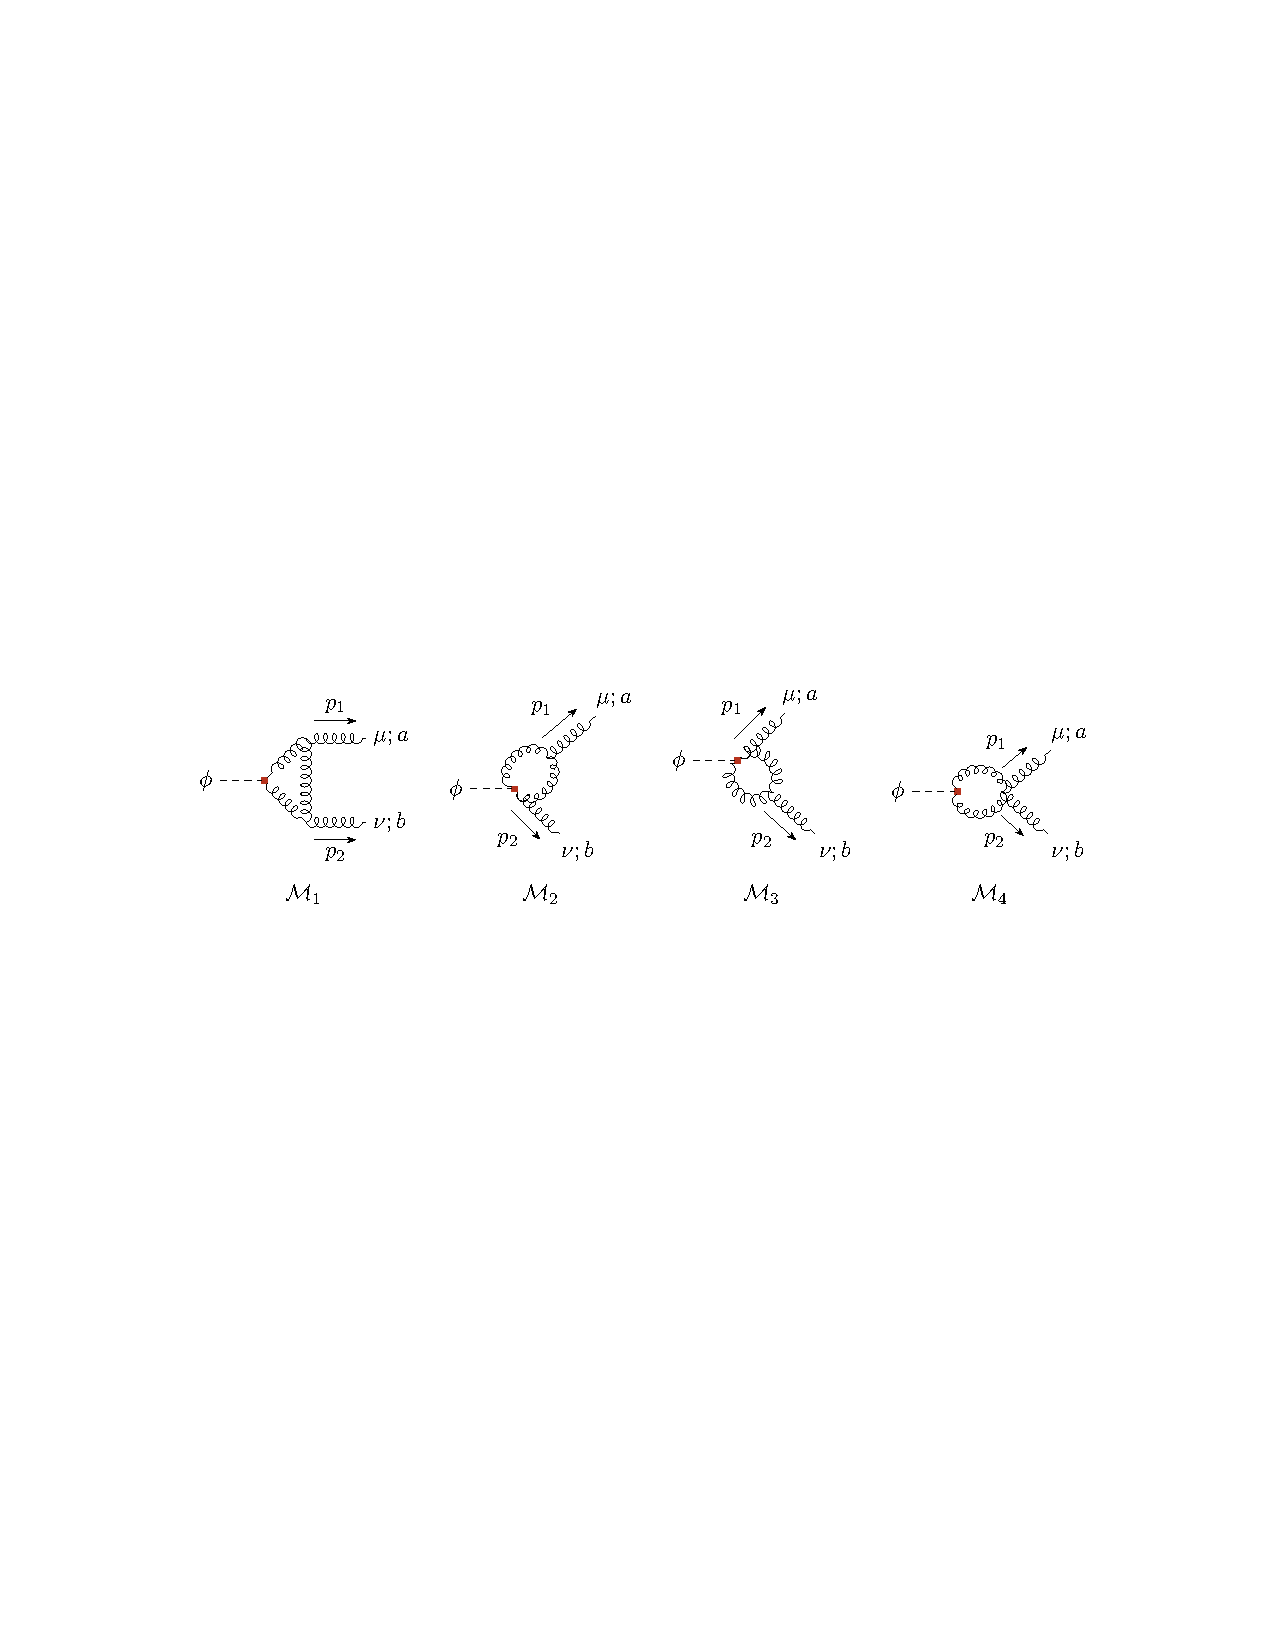
\includegraphics[width = \textwidth]{images/ALP_diagrams_phiGG.pdf}
\caption[Feynman diagrams renormalizing the vertex $\phi GG$]{Feynman diagrams contributing to the renormalization of the vertex $\phi GG$.}
\label{fig:ALPPhiGGdiagB}
\end{figure}

\begin{figure}[h!tb]
\centering
\begin{tikzpicture}
	\begin{feynman}[small]
	\node [BrickRed, square dot] (b);
    \vertex [above left=1.5cm of b] (a) {$\phi$};
    \vertex [below left=0.75cm of b] (c) ;
    \vertex [above right=1.5cm of b] (d) {\(\mu;a\)};
	\vertex [below right =1.5cm of b] (e) {\(\nu;b\)} ;
    \diagram*{
    (a) -- [scalar] (b),
    (b) -- [gluon, momentum=\(p_2\)] (e),
    (b) -- [gluon, momentum=\(p_1\)] (d),
    (b) -- [gluon, half left] (c),
    (c) -- [gluon, half left] (b),
    };
	\end{feynman}
	\end{tikzpicture}
\quad
\begin{tikzpicture}
	\begin{feynman}[small]
	\vertex (a) {\(\phi\)};
	\node [BrickRed, square dot, right=  of a] (b);
	\vertex [above right = of b] (c);
	\vertex [below right=of b] (d);
	\vertex [right =  of c] (e) {\(\mu;a\)} ;
	\vertex [right =  of d] (f) {\(\nu;b\)} ;
	\diagram*{
		(a) -- [scalar] (b),
		(c) -- [fermion] (b),
		(b) -- [fermion] (d),
		(d) -- [gluon, momentum'=\(p_2\)] (f),
		(d) -- [fermion] (c),
		(c) -- [gluon, momentum=\(p_1\)] (e),
	};
	\end{feynman}
	\end{tikzpicture}
    \quad
    \begin{tikzpicture}
	\begin{feynman}[small]
	\vertex (a) {\(\phi\)};
	\node [BrickRed, square dot, right=  of a] (b);
	\vertex [above right = of b] (c);
	\vertex [below right=of b] (d);
	\vertex [right =  of c] (e) {\(\mu;a\)} ;
	\vertex [right =  of d] (f) {\(\nu;b\)} ;
	\diagram*{
		(a) -- [scalar] (b),
		(c) -- [anti fermion] (b),
		(b) -- [anti fermion] (d),
		(d) -- [gluon, momentum'=\(p_2\)] (f),
		(d) -- [anti fermion] (c),
		(c) -- [gluon, momentum=\(p_1\)] (e),
	};
	\end{feynman}
	\end{tikzpicture}
\caption[Feynman diagrams not contributing to the renormalization of the vertex $\phi GG$]{Feynman diagrams that do not contribute to the renormalization of the vertex
$\phi G G$ because they are either identically zero or because they give rise to no UV
divergences.}
\label{fig:ALPPhiGGdiagBNotDiv}
\end{figure}

We find the following divergent terms for the diagrams in Figure~\ref{fig:ALPPhiGGdiagB}:
\begin{align}
    i {\mathcal{M}_{1}}^{ab}_{\mu\nu} &= i \frac{\alpha_s}{3\pi \epsilon} \frac{\mathcal{C}_g}{\Lambda} C_A \delta^{ab}\left[ (23 + 6 \xi_G) p_{1\nu} p_{2 \mu} - (37 + 6 \xi_G) p_1\cdot p_2 g_{\mu\nu}\right]\,,\\
    i {\mathcal{M}_{2}}^{ab}_{\mu\nu} &= i \frac{\alpha_s}{2 \pi \epsilon} \frac{\mathcal{C}_g}{\Lambda} C_A \delta^{ab}(5 +  \xi_G) \left(-p_{1\nu} p_{2 \mu} + p_1\cdot p_2 g_{\mu\nu} \right)\,, \\
    i {\mathcal{M}_{3}}^{ab}_{\mu\nu} &= i \frac{\alpha_s}{2 \pi \epsilon} \frac{\mathcal{C}_g}{\Lambda} C_A \delta^{ab}(5 +  \xi_G) \left(-p_{1\nu} p_{2 \mu} + p_1\cdot p_2 g_{\mu\nu} \right)\,,\\
    i {\mathcal{M}_{4}}^{ab}_{\mu\nu} &=
    i \frac{\alpha_s}{3 \pi \epsilon} \frac{\mathcal{C}_g}{\Lambda} C_A \delta^{ab}\left(p_{1\nu} p_{2 \mu} + 13 p_1\cdot p_2 g_{\mu\nu} \right)
    \,,
\end{align}
which add up to
\begin{equation}
i \mathcal{M}^{ab}_{\mu\nu} = i \frac{\alpha_s}{\pi \epsilon}\frac{\mathcal{C}_g}{\Lambda}C_A \delta^{ab}  (3+ \xi_G) \left(p_{1\nu} p_{2\mu} - p_1 \cdot p_2 g_{\mu\nu}\right)\,,
\end{equation}
where $\xi_G$ is the gluon gauge-fixing parameter.
Therefore, from the Feynman rule for $\phi GG$,
\begin{equation}
    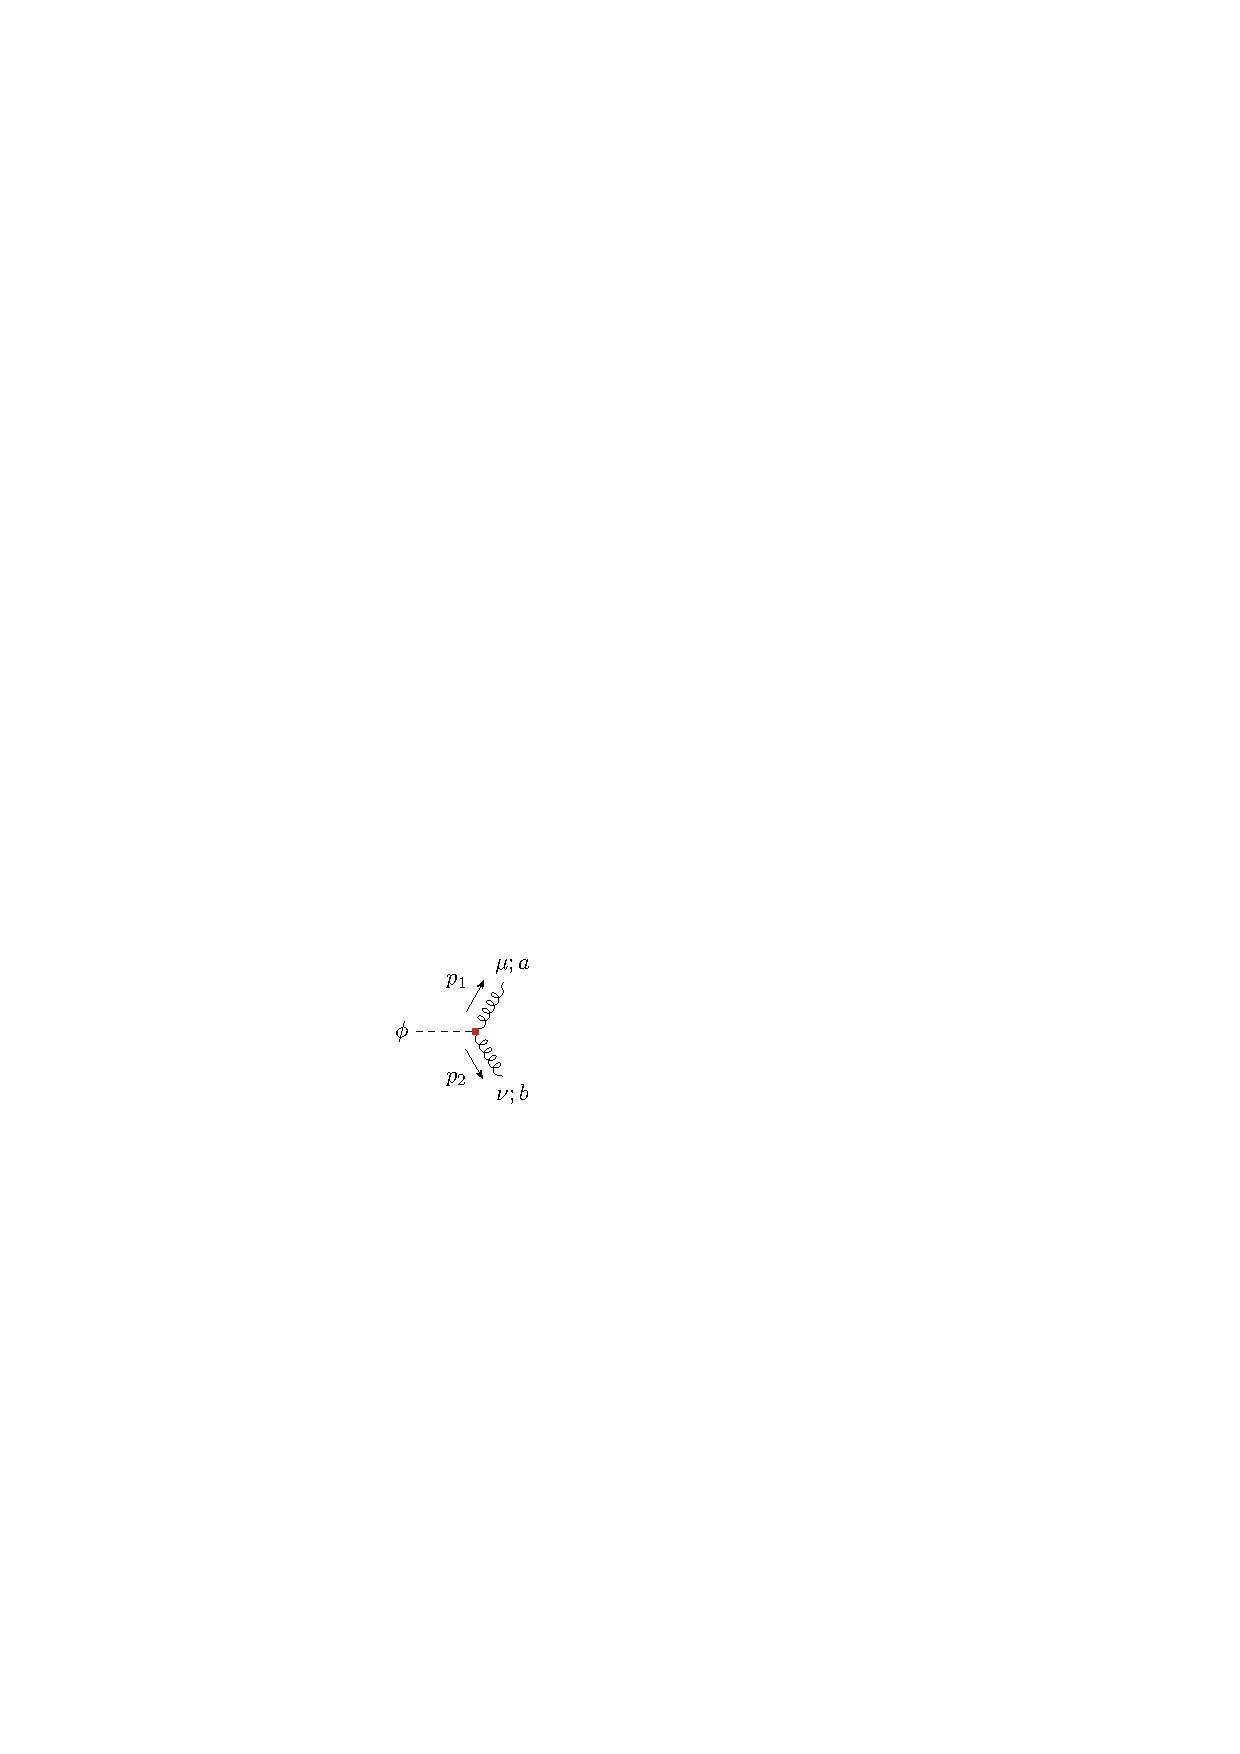
\includegraphics[valign=c,page=1]{images/ALP_FeynRules.pdf}
    = 4i \frac{\mathcal C_g}{\Lambda}\delta^{ab}(p_{1\nu} p_{2\mu} - p_1 \cdot p_2 g_{\mu\nu})\,,
\end{equation}
we can identify the renormalization factor of $\mathcal C_g$ to be
\begin{equation}
     Z_{\mathcal C_g} = 1 - \frac{\alpha_s}{4\pi\epsilon} (3+\xi_G) C_A \,.
\end{equation}
Finally, by exploiting the expression for the renormalization factor of the gluon field,
\begin{equation}
    Z_g =1+ \frac{\alpha_s}{4\pi \epsilon}\bigg[\bigg(\frac{13}{3}-\xi_G\bigg)C_A-\frac{8}{3}T_F \sum_f c_f^2 \bigg]\,,
\end{equation}
and $\mu\dv[]{}{\mu}\alpha_s=-\epsilon \alpha_s + \dotsb$, we obtain the following RGE:
\begin{equation}
    \frac{1}{\mathcal{C}_g} \mu \dv[]{\mathcal C_g}{\mu} =  -  \frac{1}{Z_{\mathcal C_g}} \mu \dv[]{Z_{\mathcal C_g}}{\mu} +  \frac{1}{Z_g} \mu \dv[]{Z_g}{\mu} = - \frac{\alpha_s}{2\pi} \bigg[ \frac{11}{3} C_A - \frac{4}{3}T_F \sum_f c_f^2 \bigg]\,.
\end{equation}
These results reproduce the ones obtained with the on-shell method, but at the expense of
computing a relatively large number of one-loop diagrams with non-trivial Lorentz and
gauge-dependent structures.
In the on-shell method, no gauge dependence is present at any level of the computation, which
requires only the convolution of one tree-level amplitude with a single form factor.

Additionally, the on-shell method allows us to manifest some hidden structures of the
computation which are jeopardized in the standard approach.
Indeed, owing to general symmetry arguments, one would expect the operator $\phi GG$ to
renormalize precisely as $GG$, and, hence, just like the infrared anomalous dimension
associated with a pair of gluons, whose long-distance dynamics is clearly dictated by their
kinetic term.
The on-shell method formalizes this property in a rather elegant way: a simple inspection of
the form of a few tree-level amplitudes directly allows us to solidly derive such a property.

Another interesting example is given by the renormalization of the Weinberg
$GG\widetilde G$ operator.
Its Feynman rule in momentum space is given by
\begin{equation}
    \includegraphics[valign=c,page=2]{images/ALP_FeynRules.pdf}
    \begin{aligned}
    &= -\frac{2}{3}\frac{d_G}{\Lambda^2}f^{abc}[\epsilon_{\mu\nu\rho\alpha}(p_1^\alpha p_2\cdot p_3+p_2^\alpha p_3\cdot p_1+p_3^\alpha p_1\cdot p_2)
    \\
    &+\epsilon_{\mu\nu\alpha\beta}(p_1-p_2)_\rho p_1^\alpha p_2^\beta  + \epsilon_{\nu\rho\alpha\beta}(p_2-p_3)_\mu p_2^\alpha p_3^\beta + \epsilon_{\rho\mu\alpha\beta}(p_3-p_1)_\nu p_3^\alpha p_1^\beta
    ]\,.
    \end{aligned}
\end{equation}
Within the standard diagrammatic framework, extracting its anomalous dimension requires
computing different diagrams, which we can conveniently classify as triangle and bubble
diagrams; see Figure~\ref{fig:ALPWeinbergdiagrams}.

\begin{figure}[h!tb]
\centering
\begin{tikzpicture}
	\begin{feynman}[small]
	\vertex (a) {\(\mu;a\)};
	\node [NavyBlue, square dot, right= 1.5cm of a] (b);
	\node [BrickRed, square dot, above right=of b] (c);
	\vertex [below right=of b] (d);
	\vertex [right=1.7cm of c] (e) {\(\nu;b\)} ;
	\vertex [right=1.3cm of d] (f) {\(\rho;c\)} ;
	\vertex (g) [below =of a] {\(\mathcal{M}_{1}^\triangle\)};
	\diagram*{
		(a) -- [gluon, rmomentum=\(p_1\)] (b),
		(c) -- [scalar] (b),
		(b) -- [gluon] (d),
		(d) -- [gluon, momentum'=\(p_3\)] (f),
		(d) -- [gluon] (c),
		(c) -- [gluon, momentum=\(p_2\)] (e),
	};
	\end{feynman}
	\end{tikzpicture}
\qquad
\begin{tikzpicture}
	\begin{feynman}[small]
	\vertex (a) {\(\mu;a\)};
	\node [BrickRed, square dot, right= 1.5cm of a] (b);
	\node [NavyBlue, square dot, above right=of b] (c);
	\vertex [below right=of b] (d);
	\vertex [right=1.7cm of c] (e) {\(\nu;b\)} ;
	\vertex [right=1.3cm of d] (f) {\(\rho;c\)} ;
	\vertex (g) [below =of a] {\(\mathcal{M}_{2}^\triangle\)};
	\diagram*{
		(a) -- [gluon, rmomentum=\(p_1\)] (b),
		(c) -- [scalar] (b),
		(b) -- [gluon] (d),
		(d) -- [gluon, momentum'=\(p_3\)] (f),
		(d) -- [gluon] (c),
		(c) -- [gluon, momentum=\(p_2\)] (e),
	};
	\end{feynman}
	\end{tikzpicture}
    \\
    \begin{tikzpicture}[baseline = (aux)]
	\begin{feynman}[small]
	\vertex (a) {\(\mu;a\)};
    \vertex [above =0.7cm of a] (aux)  ;
	\node [NavyBlue, square dot, right=1.5cm of a] (b);
	\node [BrickRed, square dot,  right=1.3 cm of b] (c);
	\vertex [above right=1.5cm of c] (e) {\(\nu;b\)} ;
	\vertex [below right=1.5cm of c] (f) {\(\rho;c\)} ;
	\vertex (g) [below = of a] {\(\mathcal{M}_{1}^\bigcirc\)};
	\diagram*{
		(a) -- [gluon, rmomentum=\(p_1\)] (b),
		(c) -- [scalar, half left] (b),
		(b) -- [gluon, half left] (c),
		(c) -- [gluon, momentum'=\(p_3\)] (f),
		(c) -- [gluon, momentum'=\(p_2\)] (e),
	};
	\end{feynman}
	\end{tikzpicture}
    \qquad
    \begin{tikzpicture}[baseline = (aux)]
	\begin{feynman}[small]
	\vertex (a) {\(\mu;a\)};
    \vertex [above =0.7cm of a] (aux)  ;
	\node [BrickRed, square dot, right=1.5cm of a] (b);
	\node [NavyBlue, square dot,  right=1.3 cm of b] (c);
	\vertex [above right=1.5cm of c] (e) {\(\nu;b\)} ;
	\vertex [below right=1.5cm of c] (f) {\(\rho;c\)} ;
	\vertex (g) [below = of a] {\(\mathcal{M}_{2}^\bigcirc\)};
	\diagram*{
		(a) -- [gluon, rmomentum=\(p_1\)] (b),
		(c) -- [scalar, half left] (b),
		(b) -- [gluon, half left] (c),
		(c) -- [gluon, momentum'=\(p_3\)] (f),
		(c) -- [gluon, momentum'=\(p_2\)] (e),
	};
	\end{feynman}
	\end{tikzpicture}
\caption[Feynman diagrams renormalizing the three-gluon Weinberg operator]{Triangle and bubble diagrams contributing to the renormalization of the three-gluon
Weinberg operator. The eight additional amplitudes with the three external gluons permuted are
omitted.}
\label{fig:ALPWeinbergdiagrams}
\end{figure}

The divergences associated with the first class of three-point diagrams are, with
$d=4-\epsilon$,
\begin{align}
    i {\mathcal M_{1}^\triangle}_{\mu\nu\rho}^{abc} &= \frac{1}{\epsilon}\frac{\mathcal C_g \widetilde{\mathcal C}_g}{3\pi^2 \Lambda^2}g_sf^{abc}\big[-\epsilon_{\mu\nu\rho\alpha}(p_1\cdot p_2+5p_2\cdot p_3)p_1^\alpha
    +\epsilon_{\mu\nu\alpha\beta}(2p_1+p_3)_\rho p_1^\alpha p_2^\beta \nonumber \\
    &\quad
    -4 \epsilon_{\mu\nu\alpha\beta}p_{2\rho} p_1^\alpha p_3^\beta
    + \epsilon_{\mu\rho\alpha\beta}(p_1+5p_3)_\nu p_1^\alpha p_2^\beta - 4 g_{\nu\rho}\epsilon_{\mu\alpha\beta\gamma}p_1^\alpha p_2^\beta p_3^\gamma
    \big]\,,\\
    i {\mathcal M_{2}^\triangle}_{\mu\nu\rho}^{abc} &= \frac{1}{\epsilon}\frac{\mathcal C_g \widetilde{\mathcal C}_g}{3\pi^2 \Lambda^2}g_sf^{abc}\big[
    \epsilon_{\mu\nu\rho\alpha}p_1^2 p_2^\alpha
    -4 \epsilon_{\mu\nu\rho\alpha}p_2^\alpha  p_1\cdot p_3
    + \epsilon_{\mu\nu\alpha\beta}(3p_1+p_3)_\rho p_1^\alpha p_2^\beta \nonumber \\
    &\quad
    - 5 \epsilon_{\mu\nu\alpha\beta}p_{1\rho} p_2^\alpha p_3^\beta
    +\epsilon_{\nu\rho\alpha\beta}(4p_3-p_1)_\mu p_1^\alpha p_2^\beta
    -5 g_{\mu\rho} \epsilon_{\nu\alpha\beta\gamma} p_1^\alpha p_2^\beta p_3^\gamma
    \big]\,.
\end{align}
By taking into account the permutations of the three external gluons, the sum of these diagrams
amounts to
\begin{equation}
i {\mathcal{M}^{\triangle}}_{\mu\nu\rho}^{abc} = \frac{1}{\epsilon}\frac{2\mathcal C_g \widetilde{\mathcal C}_g}{\pi^2 \Lambda^2}g_s f^{abc} \big[
2\epsilon_{\mu\nu\alpha\beta}p_{2\rho}
+ 2\epsilon_{\mu\rho\alpha\beta}p_{3\nu}
+\epsilon_{\nu\rho\alpha\beta}(p_3-p_2)_\mu
\big] p_2^\alpha p_3^\beta\,,
\end{equation}
where we assumed energy-momentum conservation $p_1 = - (p_2+p_3)$, the transversality
conditions for gluons, and $p_2^2=p_3^2=p_2\cdot p_3 = 0$.
The divergences associated with the two-point diagrams read instead
\begin{align}
    i {\mathcal M_{1}^\bigcirc}_{\mu\nu\rho}^{abc} &= -\frac{1}{\epsilon}\frac{\mathcal C_g \widetilde{\mathcal C}_g}{3\pi^2\Lambda^2}g_sf^{abc}(3m_\phi^2 -p_1^2)\epsilon_{\mu\nu\rho\alpha}p_1^\alpha \,,
    \\
    i {\mathcal M_{2}^\bigcirc}_{\mu\nu\rho}^{abc} &= -\frac{1}{\epsilon}\frac{\mathcal C_g \widetilde{\mathcal C}_g}{3\pi^2\Lambda^2}g_sf^{abc}
    \big[
    \epsilon_{\mu\nu\rho\alpha}[(3m_\phi^2+p_1^2)p_1^\alpha
    +3p_1^2 (p_2+p_3)^\alpha ]\nonumber \\
    &\quad -3\epsilon_{\nu\rho\alpha\beta}p_{1\mu}p_1^\alpha(p_2+p_3)^\beta
    \big]\,,
\end{align}
which are not of the desired form of the Feynman rule of $GG\widetilde G$ and can only be
interpreted as pertaining to the renormalization of the $G\widetilde G$ operator.
Indeed, the Feynman rule of the $G\widetilde G$ operator is proportional to $p_1+p_2+p_3$,
which has to vanish for on-shell gluons, as is indeed the case for these bubble contributions.
Moreover, we find that tadpole diagrams are identically vanishing.
As a consequence, the RGE associated with the Wilson coefficient $d_G$ is
\begin{equation}
    \mu\dv[]{}{\mu}d_G = -\frac{3g_s}{\pi^2}\mathcal C_g \widetilde{\mathcal C}_g\,.
\end{equation}
This reproduces the result previously reported in Eq.~\eqref{eq:ALPgammatildeG3}, but at the
price of computing more diagrams with different Lorentz structures.
On the other hand, the on-shell method only required the calculation of one form factor and one
amplitude, yielding the same result in a more transparent and elegant way.

Yet another advantage of the on-shell method is that it directly allows us to relate the
anomalous dimension for a given operator to the one of its CP counterpart, such as $\phi FF$ to
$\phi F \widetilde F$ or
$\phi \bar f f$ to $\phi \bar f i \gamma_5 f$.
In the previous example, for instance, the knowledge of the anomalous dimension for the
operator $\phi GG$ allowed us to immediately infer the one for the operator
$\phi G\widetilde G$, see Section~\ref{sec:ALPphiGG}, and similarly for $GGG$ and
$GG \widetilde{G}$, see Section~\ref{sec:ALPGGG}.
Such a duality is not manifest when working in the standard approach, where CP-dual operators
possess entirely different Lorentz structures at the level of Feynman rules, and no similarity
in the pattern of cancellations among gauge-dependent terms is present, despite the common
diagrammatic structure.

\section{Conclusions}
\label{sec:ALPconclusions}

On-shell amplitude techniques have proven to be very effective for computing the RGEs of quantum field theories~\cite{Caron-Huot:2016cwu,EliasMiro:2020tdv,Baratella:2020lzz,Jiang:2020mhe,Bern:2020ikv,Baratella:2020dvw,AccettulliHuber:2021uoa,EliasMiro:2021jgu,Baratella:2022nog,Machado:2022ozb}. 
In particular, the on-shell method~\cite{Caron-Huot:2016cwu} relates anomalous dimensions to unitarity cuts. 
As discussed in Chapter~\ref{ch:RGEmethod}, this method can also be easily applied to describe mixings among operators with different dimensions 
and to capture leading mass effects, which are of paramount importance in several phenomenological studies.

In this chapter, we have extensively applied the above techniques~\cite{Caron-Huot:2016cwu,Bresciani:2023jsu} to the one-loop renormalization of CP-violating interactions, both above and below the electroweak scale,  of an ALP with SM fields, reproducing and extending previous results~\cite{Marciano:2016yhf,DiLuzio:2020oah,Bauer:2020jbp,Chala:2020wvs,DasBakshi:2023lca,Galda:2021hbr,Galda:2023qjx}.

In particular, we  first derived the anomalous dimensions for ALP couplings with fermions, $\phi \bar f f$ and $\phi \bar f i \gamma_5 f$, which require a fermion mass insertion. This allowed us to apply the on-shell method~\cite{Caron-Huot:2016cwu} supplemented by the Higgs low-energy theorem to keep track of leading mass effects while still working in a massless formalism~\cite{Bresciani:2023jsu}. 

Then, we considered the renormalization of ALP couplings to photons and gluons, $\phi FF$ and $\phi GG$, along with their CP counterparts, $\phi F \tildee F$ and $\phi G \tildee G$, recovering the well-known result that they renormalize precisely as $FF$ and $GG$ and, hence, just like their related gauge couplings squared. 
The on-shell method shows this property in a simple and elegant way by just inspecting a few tree-level amplitudes.
Moreover, we evaluated the RGEs of operators up to dimension-six emerging after integrating out the ALP at one-loop level,  
such as the Weinberg operator $GG\tildee G$ and $GGG$, the (chromo-)magnetic and (chromo-)electric dipole moments, 
i.e., $\bar f \sigma\!\cdot\! F f$, $\bar f \sigma\!\cdot\! G f$,
$\bar f \sigma\!\cdot\! F i\gamma_5 f$, and $\bar f \sigma\!\cdot\! G i\gamma_5 f$.

A detailed derivation of the anomalous-dimension matrix was carried out both with on-shell and standard techniques, 
aiming to closely compare their virtues and shortcomings.
%
We found that on-shell methods are computationally advantageous compared to standard ones, owing to the
significantly lower and less challenging number of required contributions to be computed.
Moreover, the presence of a large number of non-Abelian gauge bosons generally renders calculations with standard techniques lengthy and computationally expensive: checks for gauge invariance were performed, often involving non-trivial cancellation of different Lorentz and gauge structures.

Remarkably, the on-shell method makes more manifest the connection between the anomalous dimension of operators related by symmetries. 
For instance, the knowledge of the anomalous dimension for the operator $\phi GG$ allowed us to immediately 
infer the one for the CP-dual operator $\phi G\tildee G$: this duality is hidden within the standard approach, where CP-dual operators have different Lorentz structures at the level of Feynman rules, and no similarity in the pattern of cancellations among gauge-dependent terms is present.

Our results were obtained by systematically evaluating all phase-space cut integrals adopting two different integration techniques, namely by angular integration~\cite{Zwiebel:2011bx} and via Stokes' theorem~\cite{Mastrolia:2009dr}. The latter, motivated by unitarity, offers the advantage of projecting directly the rational coefficient of the two-point functions out of the double cut of one-loop integrals, therefore simplifying the evaluation of anomalous dimensions.  
It would be interesting to extend Stokes integration method for the evaluation of multi-particle phase-space integrals and to apply it for the evaluation of anomalous dimensions at higher orders by unitarity cuts, which we plan for future developments.

\begin{subappendices}

%%%%%%%%%%%%%%%%%%%%%%%%%%%
\section{Amplitudes}
\label{app:ALP_amplitudes_RGE}
%%%%%%%%%%%%%%%%%%%%%%%%%%%

In this appendix, we report the amplitudes that we employed throughout the chapter, expressed
in terms of spinor-helicity variables.

\subsection{Three-Point Tree Amplitudes}

Here, the analytically continued three-point tree amplitudes in the holomorphic ($\mathsf{H}$)
and anti-holomorphic ($\mathsf{A}$) configurations, belonging to the different sectors of the
Lagrangian, are displayed on the left and on the right, respectively.
As discussed in Section~\ref{sec:3pointamplitudes}, they are completely constrained, up to an overall factor given by the coupling constant, by
locality, Poincaré invariance, and dimensional analysis~\cite{Benincasa:2007xk}.
Indeed, in full generality they read as follows:
\begin{align}
    \mathcal M_3^\mathsf{H}(1^{h_1},2^{h_2},3^{h_3}) = g_\mathsf{H} \agl{1}{2}^{a_3}\agl{2}{3}^{a_1}\agl{3}{1}^{a_2}\,, &&
    \mathcal M_3^\mathsf{A}(1^{h_1},2^{h_2},3^{h_3}) = g_\mathsf{A} \sqr{1}{2}^{\overline a_3}\sqr{2}{3}^{\overline a_1}\sqr{3}{1}^{\overline a_2}\,,
\end{align}
with $\overline a_i=-a_i$,
\begin{align}
    a_1= h_1-h_2-h_3\,,&&
    a_2= h_2-h_3-h_1\,, &&
    a_3= h_3-h_1-h_2\,,
\end{align}
and the mass dimensions of the coupling constants only depend on the helicities:
\begin{align}
    [g_\mathsf{H}]=1+h_1+h_2+h_3\,, &&
    [g_\mathsf{A}]=1-h_1-h_2-h_3\,.
\end{align}
Locality implies that the non-vanishing coupling has $[g]\le 1$. Therefore, 
the consistent configuration is determined by the sign of the sum of the helicities: three-point amplitudes have support on the holomorphic (anti-holomorphic) one if $h_1+h_2+h_3<0$ ($h_1+h_2+h_3>0$).
The case in which $h_1+h_2+h_3=0$ is trivial, as it can only correspond to a cubic scalar
interaction, where $h_1=h_2=h_3=0$.

\paragraph{\texorpdfstring{$\mathcal L_{\text{LO}}$}{L LO}.}
The lowest-order Lagrangian
\begin{equation}
    \mathcal L_{\text{LO}} = -\frac{1}{4}G_{\mu\nu}^a G^{a\mu\nu}-\frac{1}{4}F_{\mu\nu}F^{\mu\nu}+i\bar f_i \gamma^\mu D_\mu f_i - y_i h \bar f_i f_i
\end{equation}
generates
\begin{align}
    \mathcal M(1^-_{f_i},2^+_{\bar f_j},3^-_\gamma) &= \sqrt 2 e Q_f \delta^{ij} \frac{\agl{1}{3}^2}{\agl{1}{2}}\,, &
     \mathcal M(1^-_{f_i},2^+_{\bar f_j},3^+_\gamma) &= \sqrt 2 e Q_f \delta^{ij}\frac{\sqr{3}{2}^2}{\sqr{1}{2}}\,, \\
     \mathcal M(1^-_{f_i^I},2^+_{\bar f_j^J},3^-_{g^a}) &= \sqrt 2 g_s c_f T^a_{IJ}\delta^{ij} \frac{\agl{1}{3}^2}{\agl{1}{2}}\,, &
     \mathcal M(1^-_{f_i^I},2^+_{\bar f_j^J},3^+_{g^a}) &= \sqrt 2 g_s c_f T^a_{IJ} \delta^{ij}\frac{\sqr{3}{2}^2}{\sqr{1}{2}}\,, \\
     \mathcal M(1^-_{g^a},2^-_{g^b},3^+_{g^c}) &= i\sqrt 2 g_s f^{abc}\frac{\agl{1}{2}^3}{\agl{1}{3}\agl{3}{2}}\,,  &
     \mathcal M(1^+_{g^a},2^+_{g^b},3^-_{g^c}) &=-i\sqrt 2 g_s f^{abc}\frac{\sqr{1}{2}^3}{\sqr{1}{3}\sqr{3}{2}}\,,  \\
     \mathcal M(1^-_{f_i},2^-_{\bar f_j},3_h) &= - y_i\delta^{ij}\agl{1}{2}\,, &
     \mathcal M(1^+_{f_i},2^+_{\bar f_j},3_h) &= - y_i \delta^{ij} \sqr{1}{2} \,.
\end{align}

\paragraph{\texorpdfstring{$\mathcal L_{\phi}$}{L phi}.}
The ALP effective Lagrangian
\begin{equation}
    \mathcal{L}_\phi =
    \frac{\widetilde{\mathcal{C}}_\gamma}{\Lambda}\,\phi\, F\widetilde F
    + \frac{\widetilde{\mathcal{C}}_g}{\Lambda}\,\phi\, G\widetilde G
    + \mathcal{Y}^{ij}_P\,\phi\, \bar{f}_i i\gamma_5 f_j
     + \frac{\mathcal{C}_\gamma}{\Lambda}\,\phi\, FF
    + \frac{\mathcal{C}_g}{\Lambda}\,\phi\, GG
    + \mathcal{Y}^{ij}_S\,\phi\, \bar{f}_i f_j
\end{equation}
generates
\begin{align}
    \mathcal M(1^-_\gamma,2^-_\gamma,3_\phi) &= -\frac{2}{\Lambda}(\mathcal C_\gamma + i \widetilde{\mathcal{C}}_\gamma)\agl{1}{2}^2\,, &
    \mathcal M(1^+_\gamma,2^+_\gamma,3_\phi) &= -\frac{2}{\Lambda}(\mathcal C_\gamma - i \widetilde{\mathcal{C}}_\gamma)\sqr{1}{2}^2\,, \\
    \mathcal M(1^-_{g^a},2^-_{g^b},3_\phi) &= -\frac{2}{\Lambda}(\mathcal C_g + i \widetilde{\mathcal{C}}_g)\delta^{ab}\agl{1}{2}^2\,, &
    \mathcal M(1^+_{g^a},2^+_{g^b},3_\phi) &= -\frac{2}{\Lambda}(\mathcal C_g - i \widetilde{\mathcal{C}}_g)\delta^{ab}\sqr{1}{2}^2\,, \\
    \mathcal M(1^-_{f_i},2^-_{\bar f_j},3_\phi)&=(\mathcal Y_S^{ij}-i\mathcal Y_P^{ij})\agl{1}{2}\,, &
    \mathcal M(1^+_{f_i},2^+_{\bar f_j},3_\phi)&=(\mathcal Y_S^{ij}+i\mathcal Y_P^{ij})\sqr{1}{2} \,.
\end{align}

\paragraph{\texorpdfstring{$\mathcal L^{(5)}$}{L(5)}.}
The relevant dimension-five Lagrangian invariant under $SU(3)_c\times U(1)_{\text{em}}$ and
built of SM particles consists of dipole operators,
\begin{equation}
    \mathcal L^{(5)} = \frac{c_{\text{M}}^{ij}}{\Lambda}\bar f_i \sigma^{\mu\nu} f_j F_{\mu\nu} + \frac{c_{\text{E}}^{ij}}{\Lambda}\bar f_i \sigma^{\mu\nu}i\gamma_5 f_j F_{\mu\nu} + \frac{c_{\text{CM}}^{ij}}{\Lambda}\bar f_i \sigma^{\mu\nu}T^a f_j G^a_{\mu\nu} + \frac{c_{\text{CE}}^{ij}}{\Lambda}\bar f_i \sigma^{\mu\nu}i\gamma_5 T^a f_j G^a_{\mu\nu}\,,
\end{equation}
and generates
\begin{align}
    \mathcal M(1^-_{f_i},2^-_{\bar f_j},3^-_\gamma) &= \frac{2\sqrt 2}{\Lambda}C_\gamma^{ij}\agl{1}{3}\agl{2}{3}\,, &
    \mathcal M(1^+_{f_i},2^+_{\bar f_j},3^+_\gamma)&=- \frac{2\sqrt 2}{\Lambda}(C_\gamma^{ij})^*\sqr{1}{3}\sqr{2}{3}\,,  \\
    \mathcal M(1^-_{f_i^I},2^-_{\bar f_j^J},3^-_{g^a}) &= \frac{2\sqrt 2}{\Lambda}C_g^{ij}T^a_{IJ}\agl{1}{3}\agl{2}{3}\,, &
    \mathcal M(1^+_{f_i^I},2^+_{\bar f_j^J},3^+_{g^a})&= - \frac{2\sqrt 2}{\Lambda}(C_g^{ij})^*T^a_{IJ}\sqr{1}{3}\sqr{2}{3}\,,
\end{align}
with
\begin{align}
    C_\gamma^{ij}=c_{\text{M}}^{ij}-i\, c_{\text{E}}^{ij}\,, && C_g^{ij}=c_{\text{CM}}^{ij}-i\,c_{\text{CE}}^{ij}\,.
\end{align}

\paragraph{\texorpdfstring{$\mathcal L^{(6)}$}{L(6)}.}
The relevant dimension-six Lagrangian invariant under $SU(3)_c\times U(1)_{\text{em}}$ and built
of SM particles only consists of
\begin{equation}
    \mathcal L^{(6)} = \frac{D_G}{3\Lambda^2} f^{abc} G_\mu^{a, \nu} G_{\nu}^{b, \rho} G_{\rho}^{c, \mu} + \frac{d_G}{3\Lambda^2} f^{abc} G_\mu^{a, \nu} G_{\nu}^{b, \rho} \widetilde G_{\rho}^{c, \mu}
\end{equation}
and generates
\begin{align}
    \mathcal M(1^-_{g^a},2^-_{g^b},3^-_{g^c}) = i\frac{\sqrt 2}{\Lambda^2}C_Gf^{abc}\agl{1}{2}\agl{2}{3}\agl{1}{3}\,, &&
     \mathcal M(1^+_{g^a},2^+_{g^b},3^+_{g^c}) = i\frac{\sqrt 2}{\Lambda^2}C_G^* f^{abc}\sqr{2}{1}\sqr{3}{2}\sqr{3}{1}\,,
\end{align}
with
\begin{equation}
    C_G= D_G + i\, d_G\,.
\end{equation}

\subsection{Four-Point Tree Amplitudes}

Here, the four-point tree amplitudes needed for the calculations are displayed.
With the symbol $*$ we denote the region in the space of the couplings of the theory where only
the gauge couplings $e$ and $g_s$ are different from zero.
\begin{align}
     \mathcal M|_*(1^-_{f_i},2^+_{\bar f_j},3^-_\gamma,4^+_\gamma) &= -2e^2Q_f^2\delta^{ij}\frac{\agl{1}{3}\sqr{4}{2}}{\agl{1}{4}\sqr{3}{1}}\,, \\
    \mathcal M|_*(1^+_{f_i},2^-_{\bar f_j},3^-_\gamma,4^+_\gamma) &= -2e^2Q_f^2\delta^{ij}\frac{\agl{2}{3}\sqr{4}{1}}{\agl{1}{4}\sqr{3}{1}}\,, \\
    \mathcal M|_*(1^-_{f_i^I},2^+_{\bar f_j^J},3^-_{g^a},4^+_{g^b}) &= -2g_s^2c_f^2T^a_{IK}T^b_{KJ}\delta^{ij}\frac{\agl{1}{3}\sqr{4}{2}}{\agl{1}{4}\sqr{3}{1}}\,, \\
    \mathcal M|_*(1^+_{f_i^I},2^-_{\bar f_j^J},3^-_{g^a},4^+_{g^b}) &= -2g_s^2c_f^2T^b_{IK}T^a_{KJ}\delta^{ij}\frac{\agl{2}{3}\sqr{4}{1}}{\agl{1}{4}\sqr{3}{1}}\,, \\
    \mathcal M|_*(1^-_{g^a},2^-_{g^b},3^+_{g^c},4^+_{g^d}) &= -2g_s^2\agl{1}{2}^4\bigg(\frac{f^{abe}f^{cde}}{\agl{1}{2}\agl{2}{3}\agl{3}{4}\agl{4}{1}}+\frac{f^{ace}f^{bde}}{\agl{1}{3}\agl{3}{2}\agl{2}{4}\agl{4}{1}}\bigg)\,,\\
    \mathcal M|_*(1^-_{f_i^I},2^-_{\bar f_j^J},3^+_{f_k^K},4^+_{\bar f_l^L}) &= -2 (e^2 Q_f^2 \delta_{IL}\delta_{KJ}+g_s^2c_f^2T^a_{IL}T^a_{KJ}) \delta^{il}\delta^{jk} \frac{\agl{1}{2}\sqr{4}{3}}{\agl{1}{4}\sqr{4}{1}}\,, \\
    \mathcal M|_*(1^-_{f_i^I},2^+_{\bar f_j^J},3^-_{f_k^K},4^+_{\bar f_l^L}) &= +2(e^2Q_f^2\delta_{IJ}\delta_{KL}+g_s^2c_f^2T^a_{IJ}T^a_{KL})\delta^{ij}\delta^{kl} \frac{\agl{1}{3}\sqr{4}{2}}{\agl{1}{2}\sqr{2}{1}}\nonumber \\
    &\quad - 2(e^2Q_f^2\delta_{IL}\delta_{KJ}+g_s^2c_f^2T^a_{IL}T^a_{KJ}) \delta^{il}\delta^{jk} \frac{\agl{1}{3}\sqr{4}{2}}{\agl{1}{4}\sqr{4}{1}}\,, \\
    \mathcal M|_*(1^-_{f_i^I},2^+_{\bar f_j^J},3^+_{f_k^K},4^-_{\bar f_l^L}) &= +2(e^2Q_f^2\delta_{IJ}\delta_{KL}+g_s^2c_f^2T^a_{IJ}T^a_{KL})\delta^{ij}\delta^{kl} \frac{\agl{1}{4}\sqr{3}{2}}{\agl{1}{2}\sqr{2}{1}}\,,\\
    \mathcal M(1^-_{f_i},2^+_\gamma,3^-_{\bar f_j},4_h) &= -\sqrt{2} y_i \delta^{ij} e Q_f \frac{\agl{1}{3}^2}{\agl{1}{2}\agl{2}{3}}\,, \\
    \mathcal M(1^-_{f_i^I},2^+_{g^a},3^-_{\bar f_j^J},4_h) &= -\sqrt{2} y_i \delta^{ij} g_s c_f T^a_{IJ} \frac{\agl{1}{3}^2}{\agl{1}{2}\agl{2}{3}} \,,\\
    \mathcal M(1^-_{f_i},2^-_\gamma,3^+_{\bar f_j},4_\phi) &= \frac{2\sqrt 2}{\Lambda} e Q_f \delta^{ij}(\mathcal C_\gamma + i\widetilde{\mathcal C}_\gamma)\frac{\agl{1}{2}^2}{\agl{1}{3}}\,,\\
    \mathcal M(1^-_{f_i^I},2^-_{g^a},3^+_{\bar f_j^J},4_\phi) &= \frac{2\sqrt 2}{\Lambda} g_s c_f T^a_{IJ} \delta^{ij}(\mathcal C_g + i\widetilde{\mathcal C}_g)\frac{\agl{1}{2}^2}{\agl{1}{3}}\,,\\
    \mathcal M(1^-_{f_i},2^-_{\bar f_j},3^+_\gamma,4_\phi) &= -\sqrt 2 e Q_f (\mathcal Y_S^{ij}-i\mathcal Y_P^{ij})\frac{\agl{1}{2}^2}{\agl{1}{3}\agl{2}{3}} \,,\\
    \mathcal M(1^-_{f_i^I},2^-_{\bar f_j^J},3^+_{g^a},4_\phi) &= -\sqrt 2 g_s c_f T^a_{IJ} (\mathcal Y_S^{ij}-i\mathcal Y_P^{ij})\frac{\agl{1}{2}^2}{\agl{1}{3}\agl{2}{3}}\,,\\
    \mathcal M(1^-_{g^a},2^-_{g^b},3^+_{g^c},4_\phi) &= -i\frac{2\sqrt 2}{\Lambda}g_sf^{abc}(\mathcal C_g+i\widetilde{\mathcal C}_g)\frac{\agl{1}{2}^3}{\agl{1}{3}\agl{2}{3}}\,.
\end{align}

%%%%%%%%%%%%%%%%%%%%%%%%%%%
\section{Infrared Anomalous Dimensions}
\label{app:ALP_IR}
%%%%%%%%%%%%%%%%%%%%%%%%%%%

The on-shell method is not directly sensitive to the UV anomalous dimension associated
with a certain operator, $\gamma_{i\leftarrow j}$, but rather to the difference between it and
the infrared anomalous-dimension matrix, $\delta_{ij} \gamma_{i,\text{IR}}$.
Its knowledge is a necessary ingredient for the method, and therefore it is of paramount
importance to understand how to treat it properly.

There are two main approaches to infrared divergences within the scope of the on-shell method.
The first one consists in taking the infrared anomalous dimensions to be external inputs from
other computations.
For instance, at one-loop level the infrared anomalous dimension can be parameterized, in any
gauge theory, as
\begin{equation}
    \gamma_{\text{IR}} (\{p_i\}, \mu) = \frac{g^2}{4 \pi^2} \sum_{i<j} T^a_{ik} T^a_{kj} \log \frac{\mu^2}{-s_{ij}} + \sum_i \gamma_i^{\text{coll.}}\,,
\end{equation}
where $T_{ik}^a$ are the gauge-group generators acting on the particle $i$~\cite{Becher:2009cu}.
The first term of the infrared anomalous dimension stems from soft wide-angle infrared
radiation, whereas the second one describes the effects arising from hard, collinear
divergences.

Alternatively, one can compute the infrared anomalous dimensions via on-shell
techniques~\cite{Caron-Huot:2016cwu}.
Indeed, infrared divergences do not depend specifically on the gauge-invariant operator
appearing within the definition of a form factor, but only on its external states.
As a consequence, one can compute these quantities by simply considering a local,
gauge-invariant operator with a vanishing UV anomalous dimension and allowing for
two-particle interactions.
In this respect, a natural candidate is given by the energy-momentum tensor $T_{\mu\nu}$.
Since the energy-momentum tensor has to be conserved also at the quantum level, its UV
anomalous dimension has to vanish, i.e., $\gamma_{T} = 0$, and we are left with
\begin{equation}
- \gamma_{\text{IR}} \, F_T = D \, F_T\,,
\end{equation}
which implies
\begin{equation}
\label{eq:ALPMaster_Formula_LO}
    \gamma_{\text{IR}} = -\frac{D \, F_T}{F_T} = \frac{1}{\pi} \frac{(\mathcal M F_T) }{F_T}\,.
\end{equation}

In this appendix, we make use of the on-shell method to compute the infrared collinear
anomalous dimensions associated with the external particle states related to those operators
we have considered within the main text.

\subsection{\texorpdfstring{$\phi \bar f f$ and $\phi \bar f i \gamma_5 f$ Operators}{phi fbar f and phi fbar i gamma5 f Operators}}
\label{sec:ALPIRphiffb}

The infrared anomalous dimension $\gamma_{S,\text{IR}}$ associated with the operators
$\phi\, \bar f_i f_j$ and $\phi\, \bar f_i i \gamma_5 f_j$ can be computed through the
master formula
\begin{equation}
    \gamma_{S,\text{IR}} F_T^{\alpha\beta\dot\alpha\dot\beta}|_{*}(1^-_{f_i^I},2^+_{\bar f_j^J})=\frac{1}{\pi}(\mathcal M F_T^{\alpha\beta\dot\alpha\dot\beta})|_{*}(1^-_{f_i^I},2^+_{\bar f_j^J})\,,
\end{equation}
which diagrammatically reads as in Figure~\ref{fig:ALPphiffIR}.

\begin{figure}[h!tb]
\centering
\includegraphics[width=\textwidth,page=13]{images/ALP_diagrams.pdf}
\caption[Diagrammatic formula for computing $\gamma_{S,\text{IR}}$]{Diagrammatic formula for computing $\gamma_{S,\text{IR}}$.}
\label{fig:ALPphiffIR}
\end{figure}

On the left-hand side, we have the form factor of the fermion stress-energy tensor
\begin{equation}
    F_T^{\alpha\beta\dot\alpha\dot\beta}|_{*}(1_{f_i^I}^{-},2_{\bar f_j^J}^{+}) = \delta^{ij}\delta_{IJ}\mathcal T^{\alpha\beta\dot\alpha\dot\beta}_{12}\,,
\end{equation}
where we have defined
\begin{equation}
    \mathcal T^{\alpha\beta\dot\alpha\dot\beta}_{12} = \frac{1}{2}\left( \lambda_1^\alpha \lambda_1^\beta \widetilde\lambda_1^{\dot\alpha} \widetilde\lambda_2^{\dot\beta} + \lambda_1^\alpha \lambda_1^\beta \widetilde\lambda_2^{\dot\alpha} \widetilde\lambda_1^{\dot\beta} - \lambda_1^\alpha \lambda_2^\beta \widetilde\lambda_2^{\dot\alpha} \widetilde\lambda_2^{\dot\beta} - \lambda_2^\alpha \lambda_1^\beta \widetilde\lambda_2^{\dot\alpha} \widetilde\lambda_2^{\dot\beta}  \right)\,,
\end{equation}
while, on the right-hand side, the convolution is expanded allowing for all possible
intermediate states:
\begin{align}
    (\mathcal M F_T^{\alpha\beta\dot\alpha\dot\beta})|_{*}(1_{f_i^I}^{-},2_{\bar f_j^J}^{+}) &= \sum_{h_1,h_2}\int \text{dLIPS}_2\,
    \bigg[\sum_{f'}
     \mathcal M|_{*} (1_{f_i^I}^{-},2_{\bar f_j^J}^{+}; x_{f_k'^K}^{h_1},y_{\bar f_l'^L}^{h_2})F_T^{\alpha\beta\dot\alpha\dot\beta}|_{*}(x_{f_k'^K}^{h_1},y_{\bar f_l'^L}^{h_2})\nonumber \\
    &\quad + \mathcal M|_{*} (1_{f_i^I}^{-},2_{\bar f_j^J}^{+}; x_\gamma^{h_1},y_\gamma^{h_2})F_T^{\alpha\beta\dot\alpha\dot\beta}|_{*}(x_\gamma^{h_1},y_\gamma^{h_2})\nonumber \\
    &\quad+ \mathcal M|_{*} (1_{f_i^I}^{-},2_{\bar f_j^J}^{+}; x_{g^c}^{h_1},y_{g^d}^{h_2})F_T^{\alpha\beta\dot\alpha\dot\beta}|_{*}(x_{g^c}^{h_1},y_{g^d}^{h_2})
    \bigg]\,.
\end{align}
The amplitudes that give a non-vanishing contribution are
\begin{align}
    \mathcal M|_{*} (1_{f_i^I}^{-},2_{\bar f_j^J}^{+}; x_{f_k'^K}^{-},y_{\bar f_l'^L}^{+})\delta_{KL} &=
    -2\delta_{IJ}\bigg[\frac{e^2Q_f^2+C_Fg_s^2c_f^2}{\agl{1}{x}\sqr{x}{1}}\delta_{ff'}\delta^{ik}\delta^{jl} + N_{f'}\frac{e^2Q_f Q_{f'}}{\agl{1}{2}\sqr{2}{1}} \delta^{ij}\delta^{kl}\bigg]\nonumber \\&\quad\times \agl{1}{y}\sqr{x}{2}
    \,, \\
    \mathcal M|_{*} (1_{f_i^I}^{-},2_{\bar f_j^J}^{+}; x_{f_k'^K}^{+},y_{\bar f_l'^L}^{-})\delta_{KL} &=
    -2\delta_{IJ} N_{f'}e^2Q_f Q_{f'}\delta^{ij}\delta^{kl} \frac{ \agl{1}{x}\sqr{y}{2}}{\agl{1}{2}\sqr{2}{1}}\,,  \\
    \mathcal M|_*(1^-_{f_i^I},2^+_{\bar f_j^J};x^-_\gamma,y^+_\gamma) &= -2e^2Q_f^2\delta^{ij}\delta_{IJ}\frac{\agl{1}{y}\sqr{x}{2}}{\agl{1}{x}\sqr{y}{1}}\,, \\
    \mathcal M|_*(1^-_{f_i^I},2^+_{\bar f_j^J};x^+_\gamma,y^-_\gamma) &= -2e^2Q_f^2\delta^{ij}\delta_{IJ}\frac{\agl{1}{x}\sqr{y}{2}}{\agl{1}{y}\sqr{x}{1}}\,,\\
    \mathcal M|_*(1^-_{f_i^I},2^+_{\bar f_j^J};x^-_{g^a},y^+_{g^b})\delta^{ab} &= -2C_Fg_s^2c_f^2\delta^{ij}\delta_{IJ}\frac{\agl{1}{y}\sqr{x}{2}}{\agl{1}{x}\sqr{y}{1}}\,, \\
    \mathcal M|_*(1^-_{f_i^I},2^+_{\bar f_j^J};x^+_{g^a},y^-_{g^b})\delta^{ab} &= -2C_Fg_s^2c_f^2\delta^{ij}\delta_{IJ}\frac{\agl{1}{x}\sqr{y}{2}}{\agl{1}{y}\sqr{x}{1}}\,,
\end{align}
where $N_{f'}=c_{f'}N_c + (1 - c_{f'})$, namely $N_{f'}=N_c$ if $f'=q$ and $N_{f'}=1$ if
$f'=\ell$, which are respectively multiplied by
\begin{align}
    F_T^{\alpha\beta\dot\alpha\dot\beta}|_{*}(x_{f_k'^K}^{-},y_{\bar f_l'^L}^{+}) &= \delta^{kl}\delta_{KL}\mathcal T^{\alpha\beta\dot\alpha\dot\beta}_{xy} \,,&
    F_T^{\alpha\beta\dot\alpha\dot\beta}|_{*}(x_{f_k'^K}^{+},y_{\bar f_l'^L}^{-}) &= -\delta^{kl}\delta_{KL}\mathcal T^{\alpha\beta\dot\alpha\dot\beta}_{yx}\,,\\
    F_T^{\alpha\beta\dot\alpha\dot\beta}|_{*}(x_{\gamma}^{-},y_{\gamma}^{+}) &= -2\lambda_x^\alpha \lambda_x^\beta \widetilde\lambda_y^{\dot\alpha} \widetilde\lambda_y^{\dot\beta}\,, &
    F_T^{\alpha\beta\dot\alpha\dot\beta}|_{*}(x_{\gamma}^{+},y_{\gamma}^{-}) &= -2\lambda_y^\alpha \lambda_y^\beta \widetilde\lambda_x^{\dot\alpha} \widetilde\lambda_x^{\dot\beta}\,, \\
    F_T^{\alpha\beta\dot\alpha\dot\beta}|_{*}(x_{g^a}^{-},y_{g^b}^{+}) &= -2\delta^{ab}\lambda_x^\alpha \lambda_x^\beta \widetilde\lambda_y^{\dot\alpha} \widetilde\lambda_y^{\dot\beta}\,, &
    F_T^{\alpha\beta\dot\alpha\dot\beta}|_{*}(x_{g^a}^{+},y_{g^b}^{-}) &= -2\delta^{ab}\lambda_y^\alpha \lambda_y^\beta \widetilde\lambda_x^{\dot\alpha} \widetilde\lambda_x^{\dot\beta}
    \,.
\end{align}

\subparagraph{Angular integration.}
The calculation of the phase-space integral with the angular parameterization is as follows.
The amplitudes read
\begin{align}
    \mathcal M|_{*} (1_{f_i^I}^{-},2_{\bar f_j^J}^{+}; x_{f_k'^K}^{-},y_{\bar f_l'^L}^{+})\delta_{KL} &=
    2\delta_{IJ}\bigg[(e^2Q_f^2+C_Fg_s^2c_f^2)\delta_{ff'}\delta^{ik}\delta^{jl}\frac{\cos^2\theta}{\sin^2\theta}\nonumber\\ &\quad + N_{f'} e^2Q_f Q_{f'} \delta^{ij}\delta^{kl}\cos^2\theta \bigg]\,, \\
    \mathcal M|_{*} (1_{f_i^I}^{-},2_{\bar f_j^J}^{+}; x_{f_k'^K}^{+},y_{\bar f_l'^L}^{-})\delta_{KL} &= -2\delta_{IJ} N_{f'} e^2Q_f Q_{f'}\delta^{ij}\delta^{kl} \sin^2\theta\, e^{2i\varphi}\,, \\
    \mathcal M|_*(1^-_{f_i^I},2^+_{\bar f_j^J};x^-_\gamma,y^+_\gamma) &= -2e^2Q_f^2\delta^{ij}\delta_{IJ}\frac{\cos\theta}{\sin\theta}e^{-i\varphi}\,, \\
    \mathcal M|_*(1^-_{f_i^I},2^+_{\bar f_j^J};x^+_\gamma,y^-_\gamma) &= 2e^2Q_f^2\delta^{ij}\delta_{IJ}\frac{\sin\theta}{\cos\theta}e^{3i\varphi}\,, \\
    \mathcal M|_*(1^-_{f_i^I},2^+_{\bar f_j^J};x^-_{g^a},y^+_{g^b})\delta^{ab} &= -2C_Fg_s^2c_f^2\delta^{ij}\delta_{IJ}\frac{\cos\theta}{\sin\theta}e^{-i\varphi}\,, \\
    \mathcal M|_*(1^-_{f_i^I},2^+_{\bar f_j^J};x^+_{g^a},y^-_{g^b})\delta^{ab} &= 2C_Fg_s^2c_f^2\delta^{ij}\delta_{IJ}\frac{\sin\theta}{\cos\theta}e^{3i\varphi}\,,
\end{align}
and the integration in the azimuthal angle $\varphi$ yields
\begin{align}
    \int_0^{2\pi}\frac{\text{d}\varphi}{2\pi}\,F_T^{\alpha\beta\dot\alpha\dot\beta}|_{*}(x_{f_k'^K}^{-},y_{\bar f_l'^L}^{+}) &= \cos^2\theta[-1+2\cos(2\theta)]\delta^{kl}\delta_{KL}\mathcal T^{\alpha\beta\dot\alpha\dot\beta}_{12}\,,\\
    \int_0^{2\pi}\frac{\text{d}\varphi}{2\pi}\,F_T^{\alpha\beta\dot\alpha\dot\beta}|_{*}(x_{f_k'^K}^{+},y_{\bar f_l'^L}^{-})e^{2i\varphi} &= -\sin^2\theta [1+2\cos(2\theta)]\delta^{kl}\delta_{KL}\mathcal T^{\alpha\beta\dot\alpha\dot\beta}_{12}\,, \\
    \int_0^{2\pi}\frac{\text{d}\varphi}{2\pi}\,F_T^{\alpha\beta\dot\alpha\dot\beta}|_{*}(x_{\gamma}^{-},y_{\gamma}^{+})e^{-i\varphi} &= -4\cos^3\theta\sin\theta\, \mathcal T^{\alpha\beta\dot\alpha\dot\beta}_{12}\,, \\
    \int_0^{2\pi}\frac{\text{d}\varphi}{2\pi}\,F_T^{\alpha\beta\dot\alpha\dot\beta}|_{*}(x_{\gamma}^{+},y_{\gamma}^{-})e^{3i\varphi} &= 4\cos\theta\sin^3\theta\, \mathcal T^{\alpha\beta\dot\alpha\dot\beta}_{12}\,,\\
    \int_0^{2\pi}\frac{\text{d}\varphi}{2\pi}\,F_T^{\alpha\beta\dot\alpha\dot\beta}|_{*}(x_{g^a}^{-},y_{g^b}^{+})e^{-i\varphi} &= -4\delta^{ab}\cos^3\theta\sin\theta\, \mathcal T^{\alpha\beta\dot\alpha\dot\beta}_{12}\,, \\
    \int_0^{2\pi}\frac{\text{d}\varphi}{2\pi}\,F_T^{\alpha\beta\dot\alpha\dot\beta}|_{*}(x_{g^a}^{+},y_{g^b}^{-})e^{3i\varphi} &= 4\delta^{ab}\cos\theta\sin^3\theta\, \mathcal T^{\alpha\beta\dot\alpha\dot\beta}_{12}\,.
\end{align}
Therefore, the remaining integral to compute is
\begin{align}
    (\mathcal M F_T^{\alpha\beta\dot\alpha\dot\beta})|_{*}(1^-_{f_i^I},2^+_{\bar f_j^J}) &= \frac{1}{16\pi}\int_0^{\pi/2}2\sin\theta\cos\theta \,\text{d}\theta\,\bigg[2\sum_{f'}2 N_{f'}e^2Q_f Q_{f'}\sin^4\theta [1+2\cos(2\theta)]\nonumber \\
    &\quad +2\sum_{f'}2 N_{f'}e^2Q_f Q_{f'}\cos^4\theta[-1+2\cos(2\theta)]\nonumber \\
    &\quad +4(e^2Q_f^2+C_Fg_s^2c_f^2)\frac{\cos^4\theta}{\sin^2\theta}[-1+2\cos(2\theta)]\nonumber \\
    &\quad  +8(e^2Q_f^2+C_Fg_s^2c_f^2)(\cos^4\theta + \sin^4\theta)
    \bigg]F_T^{\alpha\beta\dot\alpha\dot\beta}|_{*}(1^-_{f_i^I},2^+_{\bar f_j^J})\nonumber \\
    &= \frac{1}{4\pi}(e^2Q_f^2+C_Fg_s^2c_f^2)\int_0^{\pi/2}2\sin\theta\cos\theta \,\text{d}\theta\,\bigg[\frac{\cos^4\theta}{\sin^2\theta}[-1+2\cos(2\theta)]\nonumber\\
    &\quad +2(\cos^4\theta + \sin^4\theta) \bigg]
    F_T^{\alpha\beta\dot\alpha\dot\beta}|_{*}(1^-_{f_i^I},2^+_{\bar f_j^J})\,,
\end{align}
which implies
\begin{equation}\label{eq:ALPgammaS_IR_angular}
    \gamma_{S,\text{IR}} = \frac{1}{4\pi^2}(e^2Q_f^2+C_Fg_s^2c_f^2)\int_0^{\pi/2}2\sin\theta\cos\theta \,\text{d}\theta\,\bigg[\frac{\cos^4\theta}{\sin^2\theta}[-1+2\cos(2\theta)]+2(\cos^4\theta + \sin^4\theta) \bigg]\,.
\end{equation}

\subparagraph{Stokes integration.}
The calculation of the phase-space integral with the Stokes parameterization is as follows.
The amplitudes read
\begin{align}
    \mathcal M|_{*} (1_{f_i^I}^{-},2_{\bar f_j^J}^{+}; x_{f_k'^K}^{-},y_{\bar f_l'^L}^{+})\delta_{KL} &=
2\delta_{IJ}\bigg[(e^2Q_f^2+C_Fg_s^2c_f^2)\delta_{ff'}\delta^{ik}\delta^{jl}\frac{1}{z \bar z}\nonumber\\ &\quad + N_{f'} e^2Q_f Q_{f'} \delta^{ij}\delta^{kl}\frac{1}{1+z\bar z} \bigg]\,, \\
    \mathcal M|_{*} (1_{f_i^I}^{-},2_{\bar f_j^J}^{+}; x_{f_k'^K}^{+},y_{\bar f_l'^L}^{-})\delta_{KL} &= -2\delta_{IJ} N_{f'} e^2Q_f Q_{f'}\delta^{ij}\delta^{kl}\frac{\bar z^2}{1+z\bar z}\,, \\
    \mathcal M|_*(1^-_{f_i^I},2^+_{\bar f_j^J};x^-_\gamma,y^+_\gamma) &= 2e^2Q_f^2\delta^{ij}\delta_{IJ}\frac{1}{\bar z}\,, \\
    \mathcal M|_*(1^-_{f_i^I},2^+_{\bar f_j^J};x^+_\gamma,y^-_\gamma) &= -2e^2Q_f^2\delta^{ij}\delta_{IJ}\frac{\bar z^2}{z}\,, \\
    \mathcal M|_*(1^-_{f_i^I},2^+_{\bar f_j^J};x^-_{g^a},y^+_{g^b})\delta^{ab} &= 2C_Fg_s^2c_f^2\delta^{ij}\delta_{IJ}\frac{1}{\bar z}\,, \\
    \mathcal M|_*(1^-_{f_i^I},2^+_{\bar f_j^J};x^+_{g^a},y^-_{g^b})\delta^{ab} &= -2C_Fg_s^2c_f^2\delta^{ij}\delta_{IJ}\frac{\bar z^2}{z}\,,
\end{align}
which lead to
\begin{equation}
    (\mathcal M F_T^{\alpha\beta\dot\alpha\dot\beta})|_{*}(1^-_{f_i^I},2^+_{\bar f_j^J}) =  -\frac{3}{8\pi}(e^2Q_f^2+C_Fg_s^2c_f^2) \ F_T^{\alpha\beta\dot\alpha\dot\beta}|_{*}(1^-_{f_i^I},2^+_{\bar f_j^J})
\end{equation}
and thus
\begin{equation}\label{eq:ALPgammaS_IR_stokes}
    \gamma_{S,\text{IR}} = -\frac{3}{8\pi^2}(e^2Q_f^2+C_Fg_s^2c_f^2)\,.
\end{equation}

\subsection{\texorpdfstring{$\phi FF$ and $\phi F\widetilde F$ Operators}{phi F F and phi F Ftilde Operators}}
\label{sec:ALPIRphigammagamma}

The infrared anomalous dimension $\gamma_{\gamma,\text{IR}}$ associated with the operators
$\phi FF$ and $\phi F\widetilde F$ can be computed through the master formula
\begin{equation}
    \gamma_{\gamma,\text{IR}} F_T^{\alpha\beta\dot\alpha\dot\beta}|_{*}(1^-_\gamma,2^+_\gamma)=\frac{1}{\pi}(\mathcal M F_T^{\alpha\beta\dot\alpha\dot\beta})|_{*}(1^-_\gamma,2^+_\gamma)\,,
\end{equation}
which diagrammatically reads as in Figure~\ref{fig:ALPphigammagammaIR}.

\begin{figure}[h!tb]
\centering
\includegraphics[width=\textwidth,page=11]{images/ALP_diagrams.pdf}
\caption[Diagrammatic formula for computing $\gamma_{\gamma,\text{IR}}$]{Diagrammatic formula for computing $\gamma_{\gamma,\text{IR}}$.}
\label{fig:ALPphigammagammaIR}
\end{figure}

On the left-hand side, we have the form factor of the photon stress-energy tensor
\begin{equation}
    F_T^{\alpha\beta\dot\alpha\dot\beta}|_{*}(1^-_\gamma,2^+_\gamma) = -2 \lambda_1^\alpha \lambda_1^\beta \widetilde\lambda_2^{\dot\alpha} \widetilde\lambda_2^{\dot\beta}\,,
\end{equation}
while, on the right-hand side, the convolution is expanded allowing for all possible
intermediate states:
\begin{align}
    (\mathcal M F_T^{\alpha\beta\dot\alpha\dot\beta})|_{*}(1^-_\gamma,2^+_\gamma) &= \sum_{h_1,h_2}\int \text{dLIPS}_2\,
    \bigg[
    \sum_f  \mathcal M|_{*} (1^-_\gamma,2^+_\gamma; x_{f_i}^{h_1},y_{\bar f_j}^{h_2})F_T^{\alpha\beta\dot\alpha\dot\beta}|_{*}(x_{f_i}^{h_1},y_{\bar f_j}^{h_2})\nonumber \\
    &\quad + \mathcal M|_{*} (1^-_\gamma,2^+_\gamma; x_\gamma^{h_1},y_\gamma^{h_2})F_T^{\alpha\beta\dot\alpha\dot\beta}|_{*}(x_\gamma^{h_1},y_\gamma^{h_2})\nonumber \\
    &\quad + \mathcal M|_{*} (1^-_\gamma,2^+_\gamma; x_{g^a}^{h_1},y_{g^b}^{h_2})F_T^{\alpha\beta\dot\alpha\dot\beta}|_{*}(x_{g^a}^{h_1},y_{g^b}^{h_2})
    \bigg]\,.
\end{align}
The only non-vanishing amplitudes are
\begin{align}
    \mathcal M|_{*} (1^-_\gamma,2^+_\gamma; x_{f_i}^{-},y_{\bar f_j}^{+}) &= 2e^2 Q_f^2 \delta^{ij}\frac{\agl{1}{y}\sqr{2}{x}}{\agl{2}{y}\sqr{1}{y}}\,, \\
    \mathcal M|_{*} (1^-_\gamma,2^+_\gamma; x_{f_i}^{+},y_{\bar f_j}^{-}) &= 2e^2 Q_f^2 \delta^{ij}\frac{\agl{1}{x}\sqr{2}{y}}{\agl{2}{y}\sqr{1}{y}}\,,
\end{align}
which are respectively multiplied by
\begin{align}
F_T^{\alpha\beta\dot\alpha\dot\beta}|_{*}(x_{f_i}^{-},y_{\bar f_j}^{+}) = \delta^{ij}\mathcal{T}_{xy}^{\alpha\beta\dot{\alpha}\dot{\beta}}\,, \qquad
F_T^{\alpha\beta\dot\alpha\dot\beta}|_{*}(x_{f_i}^{+},y_{\bar f_j}^{-}) = -\delta^{ij}\mathcal{T}_{yx}^{\alpha\beta\dot{\alpha}\dot{\beta}}\,.
\end{align}

\subparagraph{Angular integration.}
The calculation of the phase-space integral with the angular parameterization is as follows.
The amplitudes read
\begin{align}
    \mathcal M|_{*} (1^-_\gamma,2^+_\gamma; x_{f_i}^{-},y_{\bar f_j}^{+}) &= 2e^2 Q_f^2 \delta^{ij}\frac{\cos\theta}{\sin\theta}e^{i\varphi}\,, \\
    \mathcal M|_{*} (1^-_\gamma,2^+_\gamma; x_{f_i}^{+},y_{\bar f_j}^{-}) &= -2e^2 Q_f^2 \delta^{ij}\frac{\sin\theta}{\cos\theta}e^{3i\varphi}\,,
\end{align}
and the integration in the azimuthal angle $\varphi$ yields
\begin{align}
    \int_0^{2\pi}\frac{\text{d}\varphi}{2\pi}\,F_T^{\alpha\beta\dot\alpha\dot\beta}|_{*}(x_{f_i}^{-},y_{\bar f_j}^{+})e^{i\varphi} &= -2\delta^{ij}\lambda_1^\alpha \lambda_1^\beta \widetilde\lambda_2^{\dot\alpha} \widetilde\lambda_2^{\dot\beta} \cos^3\theta\sin\theta\,,  \\
    \int_0^{2\pi}\frac{\text{d}\varphi}{2\pi}\,F_T^{\alpha\beta\dot\alpha\dot\beta}|_{*}(x_{f_i}^{+},y_{\bar f_j}^{-})e^{3i\varphi} &=2\delta^{ij}\lambda_1^\alpha \lambda_1^\beta \widetilde\lambda_2^{\dot\alpha} \widetilde\lambda_2^{\dot\beta} \cos\theta\sin^3\theta \,.
\end{align}
Therefore, the remaining integral to compute is
\begin{align}
    (\mathcal M F_T^{\alpha\beta\dot\alpha\dot\beta})|_{*}(1^-_\gamma,2^+_\gamma) &= -4e^2 \lambda_1^\alpha \lambda_1^\beta \widetilde\lambda_2^{\dot\alpha} \widetilde\lambda_2^{\dot\beta}\frac{1}{8\pi}\int_0^{\pi/2}2\sin\theta\cos\theta \,\text{d}\theta\, (\cos^4\theta+\sin^4\theta)\sum_fQ_f^2 \nonumber \\
    &= -2\lambda_1^\alpha \lambda_1^\beta \widetilde\lambda_2^{\dot\alpha} \widetilde\lambda_2^{\dot\beta}\frac{e^2}{6\pi}\sum_fQ_f^2\,,
\end{align}
which implies
\begin{equation}\label{eq:ALPgammaIRphoton}
    \gamma_{\gamma,\text{IR}} = \frac{e^2}{6\pi^2} \sum_f Q_f^2\,.
\end{equation}

\subparagraph{Stokes integration.}
By exploiting the Stokes parameterization, the amplitudes read
\begin{align}
    \mathcal M|_{*} (1^-_\gamma,2^+_\gamma; x_{f_i}^{-},y_{\bar f_j}^{+}) &= -2e^2 Q_f^2 \delta^{ij}\frac{1}{z}\,, \\
    \mathcal M|_{*} (1^-_\gamma,2^+_\gamma; x_{f_i}^{+},y_{\bar f_j}^{-}) &= 2e^2 Q_f^2 \delta^{ij}\frac{\bar z^2}{z}\,,
\end{align}
and plugging everything together we obtain
\begin{align}
    (\mathcal M F_T^{\alpha\beta\dot\alpha\dot\beta})|_{*}(1^-_\gamma,2^+_\gamma)
    &= -2\lambda_1^\alpha \lambda_1^\beta \widetilde\lambda_2^{\dot\alpha} \widetilde\lambda_2^{\dot\beta}\frac{e^2}{6\pi}\sum_fQ_f^2\,,
\end{align}
which implies Eq.~\eqref{eq:ALPgammaIRphoton}.

\subsection{\texorpdfstring{$\phi GG$ and $\phi G\widetilde G$ Operators}{phi G G and phi G Gtilde Operators}}
\label{sec:ALPIRphigg}

The infrared anomalous dimension $\gamma_{g,\text{IR}}$ associated with the operators $\phi GG$
and $\phi G\widetilde G$ can be computed through the master formula
\begin{equation}
    \gamma_{g,\text{IR}} F_T^{\alpha\beta\dot\alpha\dot\beta}|_{*}(1^-_{g^a},2^+_{g^b})=\frac{1}{\pi}(\mathcal M F_T^{\alpha\beta\dot\alpha\dot\beta})|_{*}(1^-_{g^a},2^+_{g^b})\,,
\end{equation}
which diagrammatically reads as in Figure~\ref{fig:ALPphigluongluonIR}.

\begin{figure}[h!tb]
\centering
\includegraphics[width=\textwidth,page=12]{images/ALP_diagrams.pdf}
\caption[Diagrammatic formula for computing $\gamma_{g,\text{IR}}$]{Diagrammatic formula for computing $\gamma_{g,\text{IR}}$.}
\label{fig:ALPphigluongluonIR}
\end{figure}

On the left-hand side, we have the form factor of the gluon stress-energy tensor
\begin{equation}
    F_T^{\alpha\beta\dot\alpha\dot\beta}|_{*}(1^-_{g^a},2^+_{g^b}) = -2 \delta^{ab} \lambda_1^\alpha \lambda_1^\beta \widetilde\lambda_2^{\dot\alpha} \widetilde\lambda_2^{\dot\beta}\,,
\end{equation}
while, on the right-hand side, the convolution is expanded allowing for all possible
intermediate states:
\begin{align}
    (\mathcal M F_T^{\alpha\beta\dot\alpha\dot\beta})|_{*}(1^-_{g^a},2^+_{g^b}) &= \sum_{h_1,h_2}\int \text{dLIPS}_2\,
    \bigg[
    \sum_f  \mathcal M|_{*} (1^-_{g^a},2^+_{g^b}; x_{f_i^I}^{h_1},y_{\bar f_j^J}^{h_2})F_T^{\alpha\beta\dot\alpha\dot\beta}|_{*}(x_{f_i^I}^{h_1},y_{\bar f_j^J}^{h_2})\nonumber \\
    &\quad + \mathcal M|_{*} (1^-_{g^a},2^+_{g^b}; x_\gamma^{h_1},y_\gamma^{h_2})F_T^{\alpha\beta\dot\alpha\dot\beta}|_{*}(x_\gamma^{h_1},y_\gamma^{h_2})\nonumber \\
    &\quad + \mathcal M|_{*} (1^-_{g^a},2^+_{g^b}; x_{g^c}^{h_1},y_{g^d}^{h_2})F_T^{\alpha\beta\dot\alpha\dot\beta}|_{*}(x_{g^c}^{h_1},y_{g^d}^{h_2})
    \bigg]\,.
\end{align}
The amplitudes that give a non-vanishing contribution are
\begin{align}
    \mathcal M|_*(1^-_{g^a},2^+_{g^b};x_{f_i^I}^{-},y_{\bar f_j^J}^{+})\delta_{IJ} &= 2T_Fg_s^2c_f^2\delta^{ij}\delta^{ab}\frac{\agl{1}{y}\sqr{x}{2}}{\agl{2}{y}\sqr{y}{1}}\,, \\
    \mathcal M|_*(1^-_{g^a},2^+_{g^b};x_{f_i^I}^{+},y_{\bar f_j^J}^{-})\delta_{IJ} &= 2T_Fg_s^2c_f^2\delta^{ij}\delta^{ab}\frac{\agl{1}{x}\sqr{y}{2}}{\agl{2}{y}\sqr{y}{1}}\,,\\
    \mathcal M|_* (1^-_{g^a},2^+_{g^b};x_{g^c}^{-},y_{g^d}^{+}) \delta^{cd} &= -2C_A g_s^2\delta^{ab}\frac{\agl{1}{y}^4}{\agl{1}{x}\agl{x}{2}\agl{2}{y}\agl{y}{1}}\,, \\
    \mathcal M|_* (1^-_{g^a},2^+_{g^b};x_{g^c}^{+},y_{g^d}^{-}) \delta^{cd} &= -2C_A g_s^2\delta^{ab}\frac{\agl{1}{x}^4}{\agl{1}{x}\agl{x}{2}\agl{2}{y}\agl{y}{1}}\,,
\end{align}
which are respectively multiplied by
\begin{align}
&
F_T^{\alpha\beta\dot\alpha\dot\beta}|_{*}(x_{f_i^I}^{-},y_{\bar f_j^J}^{+}) = \delta^{ij}\delta_{IJ}\mathcal{T}_{xy}^{\alpha\beta\dot{\alpha}\dot{\beta}}\,,
\qquad & &
F_T^{\alpha\beta\dot\alpha\dot\beta}|_{*}(x_{f_i^I}^{+},y_{\bar f_j^J}^{-}) = -\delta^{ij}\delta_{IJ}\mathcal{T}_{yx}^{\alpha\beta\dot{\alpha}\dot{\beta}}\,,
\\
&
F_T^{\alpha\beta\dot\alpha\dot\beta}|_{*}(x_{g^c}^{-},y_{g^d}^{+}) = -2\delta^{cd}\lambda_x^\alpha \lambda_x^\beta \widetilde\lambda_y^{\dot\alpha} \widetilde\lambda_y^{\dot\beta}\,,
& & F_T^{\alpha\beta\dot\alpha\dot\beta}|_{*}(x_{g^c}^{+},y_{g^d}^{-}) = -2\delta^{cd}\lambda_y^\alpha \lambda_y^\beta \widetilde\lambda_x^{\dot\alpha} \widetilde\lambda_x^{\dot\beta}\,.
\end{align}

\subparagraph{Angular integration.}
The calculation of the phase-space integral with the angular parameterization is as follows.
The amplitudes read
\begin{align}
    \mathcal M|_*(1^-_{g^a},2^+_{g^b};x_{f_i^I}^{-},y_{\bar f_j^J}^{+})\delta_{IJ} &= 2T_Fg_s^2c_f^2\delta^{ij}\delta^{ab}\frac{\cos\theta}{\sin\theta}e^{i\varphi}\,, \\
    \mathcal M|_*(1^-_{g^a},2^+_{g^b};x_{f_i^I}^{+},y_{\bar f_j^J}^{-})\delta_{IJ} &= -2T_Fg_s^2c_f^2\delta^{ij}\delta^{ab}\frac{\sin\theta}{\cos\theta}e^{3i\varphi}\,,\\
    \mathcal M|_* (1^-_{g^a},2^+_{g^b};x_{g^c}^{-},y_{g^d}^{+}) \delta^{cd} &= 2C_A g_s^2\delta^{ab}\frac{\cos^2\theta}{\sin^2\theta}\,, \\
    \mathcal M|_* (1^-_{g^a},2^+_{g^b};x_{g^c}^{+},y_{g^d}^{-}) \delta^{cd} &= 2C_A g_s^2\delta^{ab}\frac{\sin^2\theta}{\cos^2\theta}e^{4i\varphi}\,,
\end{align}
and the integration in the azimuthal angle $\varphi$ yields
\begin{align}
    \int_0^{2\pi}\frac{\text{d}\varphi}{2\pi}\,F_T^{\alpha\beta\dot\alpha\dot\beta}|_{*}(x_{f_i^I}^{-},y_{\bar f_j^J}^{+})e^{i\varphi} &= -2\delta^{ij}\delta_{IJ}\lambda_1^\alpha \lambda_1^\beta \widetilde\lambda_2^{\dot\alpha} \widetilde\lambda_2^{\dot\beta}\cos^3\theta\sin\theta\,, \\
    \int_0^{2\pi}\frac{\text{d}\varphi}{2\pi}\,F_T^{\alpha\beta\dot\alpha\dot\beta}|_{*}(x_{f_i^I}^{+},y_{\bar f_j^J}^{-})e^{3i\varphi} &=2\delta^{ij}\delta_{IJ}\lambda_1^\alpha \lambda_1^\beta \widetilde\lambda_2^{\dot\alpha} \widetilde\lambda_2^{\dot\beta} \cos\theta\sin^3\theta\,, \\
    \int_0^{2\pi}\frac{\text{d}\varphi}{2\pi}\,F_T^{\alpha\beta\dot\alpha\dot\beta}|_{*}(x_{g^c}^{-},y_{g^d}^{+}) &= -2\delta^{cd}\lambda_1^\alpha \lambda_1^\beta \widetilde\lambda_2^{\dot\alpha} \widetilde\lambda_2^{\dot\beta}\cos^4\theta\,, \\
    \int_0^{2\pi}\frac{\text{d}\varphi}{2\pi}\,F_T^{\alpha\beta\dot\alpha\dot\beta}|_{*}(x_{g^c}^{+},y_{g^d}^{-})e^{4i\varphi} &= -2\delta^{cd}\lambda_1^\alpha \lambda_1^\beta \widetilde\lambda_2^{\dot\alpha} \widetilde\lambda_2^{\dot\beta}\sin^4\theta\,.
\end{align}
Therefore, the remaining integral to compute is
\begin{multline}
    (\mathcal M F_T^{\alpha\beta\dot\alpha\dot\beta})|_{*}(1^-_{g^a},2^+_{g^b}) = -2 \delta^{ab} \lambda_1^\alpha \lambda_1^\beta \widetilde\lambda_2^{\dot\alpha} \widetilde\lambda_2^{\dot\beta}g_s^2\frac{1}{8\pi}\int_0^{\pi/2}2\sin\theta\cos\theta \,\text{d}\theta \,\\ \times \bigg[2T_F(\cos^4\theta + \sin^4\theta)\sum_f c_f^2 + C_A\frac{\cos^8\theta + \sin^8\theta}{\cos^2\theta \sin^2\theta}\bigg]\,,
\end{multline}
which implies
\begin{equation}\label{eq:ALPgammaIRgluon_angular}
    \gamma_{g,\text{IR}} =T_F\frac{g_s^2}{6\pi^2}\sum_f c_f^2 +C_A\frac{g_s^2}{8\pi^2}\int_0^{\pi/2}2\sin\theta\cos\theta \,\text{d}\theta \, \frac{\cos^8\theta + \sin^8\theta}{\cos^2\theta \sin^2\theta} \,.
\end{equation}

\subparagraph{Stokes integration.}
Using the Stokes parameterization, the amplitudes read
\begin{align}
    \mathcal M|_*(1^-_{g^a},2^+_{g^b};x_{f_i^I}^{-},y_{\bar f_j^J}^{+})\delta_{IJ} &= -2T_Fg_s^2c_f^2\delta^{ij}\delta^{ab}\frac{1}{z}\,, \\
    \mathcal M|_*(1^-_{g^a},2^+_{g^b};x_{f_i^I}^{+},y_{\bar f_j^J}^{-})\delta_{IJ} &= 2T_Fg_s^2c_f^2\delta^{ij}\delta^{ab}\frac{\bar z^2}{z}\,,\\
    \mathcal M|_* (1^-_{g^a},2^+_{g^b};x_{g^c}^{-},y_{g^d}^{+}) \delta^{cd} &= 2C_A g_s^2\delta^{ab}\frac{1}{z \bar z}\,, \\
    \mathcal M|_* (1^-_{g^a},2^+_{g^b};x_{g^c}^{+},y_{g^d}^{-}) \delta^{cd} &=2C_A g_s^2\delta^{ab}\frac{ \bar z^3}{z }\,,
\end{align}
and yield
\begin{equation}\label{eq:ALPgammaIRgluon_stokes}
    \gamma_{g,\text{IR}} =-\frac{g_s^2}{8\pi^2}\bigg(\frac{11}{3}C_A -\frac{4}{3}T_F\sum_fc_f^2\bigg) \,.
\end{equation}

\end{subappendices}
